\documentclass{book}
\usepackage{a4wide}

%% possible fonts -- in order of preference
%%\usepackage{palatino}
\usepackage{bookman}
%%\usepackage{charter}
%%\usepackage{newcent}
%%\usepackage{times}
%%\usepackage{avant}
%%\usepackage{helvet}
%%\usepackage{sans}
%%\usepackage{chancery}

\usepackage[T1]{fontenc}
\usepackage{setspace}
\usepackage{ifpdf}
\usepackage{makeidx}
\usepackage{longtable}  %% page wrapping table environment
\usepackage{colortbl}   %% colors for tables
\usepackage{fancyvrb}   %% the "Verbatim" environment
\usepackage{fancyhdr}   %% custom headers and footers
\usepackage{multicol}
\usepackage{listings}   %% source code listings with syntax highlight (lstxxx commands)
\usepackage[tight]{shorttoc}   %% for generating a second table of contents, only containing chapter titles
\usepackage{bytefield}  %% for drawing protocol frames
\usepackage{paralist}   %% for compact lists
\usepackage[nottoc]{tocbibind}  %% makes Bibliography and Index show up in TOC
\settocbibname{References}

\setlength{\textwidth}{160mm}
%\setlength{\oddsidemargin}{12.5mm}
%\setlength{\evensidemargin}{12.5mm}
%\setlength{\topmargin}{0mm}
\setlength{\textheight}{220mm}
%\setlength{\parskip}{1ex}
%\setlength{\parindent}{5ex}

\renewcommand{\bottomfraction}{0.9}
\renewcommand{\topfraction}{0.9}
\renewcommand{\floatpagefraction}{0.9}

%% try to cure overfull hboxes
%% \tolerance=500

%% for navigation in dvi files, only needed by old teTeX versions
%%\usepackage{srcltx}

%% try this for spell checking: cat ess2002.tex | ispell -l -t -a | sort | uniq | more

%%
%% The following snippet changes the horizontal spacing between the number and
%% the title in the table of contents.
%%
%% http://tex.stackexchange.com/questions/33841/how-to-modify-the-space-between-the-numbers-and-text-of-sectioning-titles-in-the
%%
\makeatletter
 \renewcommand*\l@section{\@dottedtocline{1}{2em}{3em}}
 \renewcommand*\l@subsection{\@dottedtocline{2}{5em}{4em}}
\renewcommand*\l@chapter[2]{%
  \ifnum \c@tocdepth >\m@ne
    \addpenalty{-\@highpenalty}%
    \vskip 1.0em \@plus\p@
    \setlength\@tempdima{2em}%
    \begingroup
      \parindent \z@ \rightskip \@pnumwidth
      \parfillskip -\@pnumwidth
      \leavevmode \bfseries
      \advance\leftskip\@tempdima
      \hskip -\leftskip
      #1\nobreak\hfil \nobreak\hb@xt@\@pnumwidth{\hss #2}\par
      \penalty\@highpenalty
    \endgroup
  \fi}
\makeatother

%%
%% OMNeT++ logo, use as {\opp}
%%
\makeatletter
%%\DeclareRobustCommand{\omnetpp}{OM\-NeT\kern-.18em++\@}
\DeclareRobustCommand{\omnetpp}{OMNeT++\@}
\makeatother

\newcommand{\opp}{\omnetpp}

%%
%% PDF Header
%%
% note: \ifpdf now comes from the ifpdf package
%\newif\ifpdf
%\ifx\pdfoutput\undefined
%  \pdffalse
%\else
%  \pdfoutput=1
%  \pdftrue
%\fi
%% PDF-Info
\ifpdf
  \usepackage[pdftex]{graphicx}
  \usepackage[plainpages=false,linktocpage,bookmarksnumbered=true,pdftex]{hyperref}   %% automatic hyperlinking
  \pdfcompresslevel=9
  \pdfinfo{/Author (Andras Varga and others)
    /Title (INET Framework Manual)
    /Subject ()
    /Keywords (INET, INETMANET, OMNeT++, manual)}
\else
  \usepackage{graphicx}
  \usepackage[plainpages=false]{hyperref}   %% automatic hyperlinking
\fi

%%
%% Draft conditional to include unfinished parts
%%
\newif\ifdraft
\draftfalse %% uncomment for final version
%\drafttrue %% uncomment for draft version

%%
%% Generate Index
%%
\makeindex


%%
%% Link colors (hyperref package)
%%
\definecolor{MyDarkBlue}{rgb}{0.16,0.16,0.5}
%% XXX the next line apparently screws up all links except in TOC! they'll be colored nicely, but won't work.
%\hypersetup{
%    colorlinks=true,
%    linkcolor=MyDarkBlue,
%    anchorcolor=MyDarkBlue,
%    citecolor=MyDarkBlue,
%    filecolor=MyDarkBlue,
%    menucolor=MyDarkBlue,
%    runcolor=MyDarkBlue,
%    urlcolor=blue,
%}

%%
%% Heading and Footer
%%
\pagestyle{fancy}
\fancyhf{}
\renewcommand{\footrulewidth}{0.5pt}
\renewcommand{\chaptermark}[1]{\markboth{#1}{}}
\lhead{INET Framework Manual -- \leftmark}
\rfoot{\thepage}

%% this is used for chapter start pages
\fancypagestyle{plain}{
    \rfoot{\thepage}
}

%%
%% Use \begin{graybox}...\end{graybox} for notes
%%
\definecolor{MyGray}{rgb}{0.85,0.85,1.0}
\makeatletter\newenvironment{graybox}%
   {\begin{flushright}\begin{lrbox}{\@tempboxa}\begin{minipage}[r]{0.95\textwidth}}%
   {\end{minipage}\end{lrbox}\colorbox{MyGray}{\usebox{\@tempboxa}}\end{flushright}}%
\makeatother


\newenvironment{note}{\begin{graybox}\textbf{NOTE: }}{\end{graybox}}
\newenvironment{warning}{\begin{graybox}\textbf{WARNING: }}{\end{graybox}}
\newenvironment{caution}{\begin{graybox}\textbf{CAUTION: }}{\end{graybox}}
\newenvironment{rationale}{\begin{graybox}\textbf{Rationale: }}{\end{graybox}}
\newenvironment{important}{\begin{graybox}\textbf{IMPORTANT: }}{\end{graybox}}

%%
%% Set up listings package
%%
\lstloadlanguages{C++,make,perl,tcl,XML,R,Matlab}

%% See listings.pdf,pp20
\lstdefinelanguage{NED} {
    morekeywords={allowunconnected,bool,channel,channelinterface,connections,const,
                  default,double,extends,false,for,gates,if,import,index,inout,input,
                  int,like,module,moduleinterface,network,output,package,parameters,
                  property,simple,sizeof,string,submodules,this,true,types,volatile,
                  xml,xmldoc},
    sensitive=true,
    morecomment=[l]{//},
    morestring=[b]",
}
\lstdefinelanguage{MSG} {
    morekeywords={abstract,bool,char,class,cplusplus,double,enum,extends,false,
                  fields,int,long,message,namespace,noncobject,packet,properties,
                  readonly,short,string,struct,true,unsigned},
    sensitive=true,
    morecomment=[l]{//},
    morestring=[b]",
}
\lstdefinelanguage{inifile} {
    morekeywords={},
    sensitive=true,
    morecomment=[l]{\#},
    morestring=[b]",
}
\lstdefinelanguage{pseudocode} {
    morekeywords={if,then,else,otherwise,whenever,while},
    sensitive=true,
    morecomment=[l]{//},
    morestring=[b]",
    mathescape=true,
}

%% thick ruler on the left; also, designate backtick as LaTeX escape character
%% (e.g. \opp needs to be written as `\opp` inside listing blocks)
\lstset{
    escapechar=`,
    basicstyle=\ttfamily,
    showstringspaces=false,
    frame=leftline,
    framesep=10pt,
    framerule=3pt,
    xleftmargin=15pt
}

\definecolor{NEDRulerColor}{rgb}{0.8,1.0,0.8}  % pale green
\definecolor{MSGRulerColor}{rgb}{0.8,1.0,0.8}  % pale green
\definecolor{CPPRulerColor}{rgb}{0.8,0.8,1.0}  % pale blue
\definecolor{IniRulerColor}{rgb}{0.9,0.9,0.2}  % pale yellow
\definecolor{FileListingRulerColor}{rgb}{0.85,0.85,0.85}  % grey
%\definecolor{CommandLineRulerColor}{rgb}{0.9,0.9,0.2}
\definecolor{PseudoCodeRulerColor}{rgb}{0.0,1.0,1.0}  % cyan

%% See listings.pdf,pp39
\lstnewenvironment{ned}
    {\lstset{language=NED,rulecolor=\color{NEDRulerColor}}}
    {}
\lstnewenvironment{msg}
    {\lstset{language=MSG,rulecolor=\color{MSGRulerColor}}}
    {}
\lstnewenvironment{cpp}
    {\lstset{language=C++,rulecolor=\color{CPPRulerColor}}}
    {}
\lstnewenvironment{inifile}
    {\lstset{language=inifile,rulecolor=\color{IniRulerColor}}}
    {}
\lstnewenvironment{filelisting}
    {\lstset{language={},rulecolor=\color{FileListingRulerColor}}}
    {}
\lstnewenvironment{commandline}
    {\lstset{language={},framesep=11pt,framerule=1pt,xleftmargin=16pt}}
    {}
\lstnewenvironment{pseudocode}
    {\lstset{language=pseudocode,rulecolor=\color{PseudoCodeRulerColor}}}
    {}

%%
%% some customization
%%
\setlength{\parindent}{0pt}
\setlength{\parskip}{1ex}

%%
%% Shortcuts
%%
\newcommand{\appendixchapter}{\chapter} %% html converter needs to know which chapters are appendices

\newcommand{\tbf}{\textbf} %% bold faced text
\newcommand{\ttt}{\texttt} %% type writer font text

\newcommand{\tab}{\hspace*{5mm}} %% tabulator settings

\newcommand{\new}{$^{New!}$}
\newcommand{\changed}{$^{Changed!}$}

%% Colordefinition for table header rows (requires package colortbl)
\newcommand{\tabheadcol}{\rowcolor[gray]{0.8}}

%%
%% Module parameters list
%%
\newenvironment{params}{\begin{itemize}}{\end{itemize}}
\newcommand{\param}[2]{\item \fpar{#1}: #2}

%%
%% Function/Class/Macro/Variable/Program/Parameter/Define names
%%
%% Write the names in type writer font and do an index entry
%% Allows word wrap by automatic hyphenation
%%
%% Usage: \ffunc{take()}
%%    or: \ffunc[take()]{take(obj)}
%% the second form uses the bracketed word for the index entry
%%

%% NED type names
\newcommand{\nedtype}[2][\DefaultOpt]{\def\DefaultOpt{#2}%
  \index{#1}%
  \texttt{\hyphenchar\font=`\-\relax#2}}

%% MSG type names
\newcommand{\msgtype}[2][\DefaultOpt]{\def\DefaultOpt{#2}%
  \index{#1}%
  \texttt{\hyphenchar\font=`\-\relax#2}}

%% Function names
\newcommand{\ffunc}[2][\DefaultOpt]{\def\DefaultOpt{#2}%
  \index{#1}%
  \texttt{\hyphenchar\font=`\-\relax#2}}

%% Class names
\newcommand{\cppclass}[2][\DefaultOpt]{\def\DefaultOpt{#2}%
  \index{#1}%
  \texttt{\hyphenchar\font=`\-\relax#2}}

%% Macro names
\newcommand{\fmac}[2][\DefaultOpt]{\def\DefaultOpt{#2}%
  \index{#1}%
  \texttt{\hyphenchar\font=`\-\relax#2}}

%% Variable names
\newcommand{\fvar}[2][\DefaultOpt]{\def\DefaultOpt{#2}%
  \index{#1}%
  \texttt{\hyphenchar\font=`\-\relax#2}}

%% Program names
\newcommand{\fprog}[2][\DefaultOpt]{\def\DefaultOpt{#2}%
  \index{#1}%
  \texttt{\hyphenchar\font=`\-\relax#2}}

%% Parameter names
\newcommand{\fpar}[2][\DefaultOpt]{\def\DefaultOpt{#2}%
  \index{#1}%
  \texttt{\hyphenchar\font=`\-\relax#2}}

%% Defines
\newcommand{\fdef}[2][\DefaultOpt]{\def\DefaultOpt{#2}%
  \index{#1}%
  \texttt{\hyphenchar\font=`\-\relax#2}}

%% NED/MSG properties
\newcommand{\fprop}[2][\DefaultOpt]{\def\DefaultOpt{#2}%
  \index{#1}%
  \texttt{\hyphenchar\font=`\-\relax#2}}

%% Keywords (NED, MSG)
\newcommand{\fkeyword}[2][\DefaultOpt]{\def\DefaultOpt{#2}%
  \index{#1}%
  \textbf{\texttt{\hyphenchar\font=`\-\relax#2}}}

%% Configuration options
\newcommand{\fconfig}[2][\DefaultOpt]{\def\DefaultOpt{#2}%
  \index{#1}%
  \textbf{\texttt{\hyphenchar\font=`\-\relax#2}}}

%% File names
\newcommand{\ffilename}[2][\DefaultOpt]{\def\DefaultOpt{#2}%
  \index{#1}%
  \texttt{\hyphenchar\font=`\-\relax#2}}

%% Signals
\newcommand{\fsignal}[2][\DefaultOpt]{\def\DefaultOpt{#2}%
  \index{#1}%
  \texttt{\hyphenchar\font=`\-\relax#2}}

\newcommand{\fgate}[1]{\texttt{\hyphenchar\font=`\-\relax#1}}

%% do not number subsubsections
%\setcounter{secnumdepth}{4}

% limit the depth of TOC
\setcounter{tocdepth}{2}

%%
%% Start of document
%%
\begin{document}

%% set the image type preference
\DeclareGraphicsExtensions{.pdf,.png}

\pagestyle{empty}
\pagenumbering{roman}

%% %%\begin{figure}[htbp]
%%\begin{center}
%%\includegraphics[width=3.648in, height=0.990in]{figures/usmanFig1}
%%\end{center}
%% %%\end{figure}

%% the following {center} is a trick -- vspace does nothing if there's
%% nothing above it in the page
\begin{center}\end{center}
\vspace{16em}
\hrule
\vspace{2em}
\begin{center}
{\HUGE INET Framework}\\
\vspace{2em}
{\Huge Developer's Guide}\\
\vspace{2em}
{\Large Version 4.0}\\
\end{center}
\vspace{2em}
\hrule

\begin{center}
\textit{\today}
\end{center}




\cleardoublepage

%%\setcounter{page}{1}
%\newpage
%%\pagenumbering{roman}

%% \shorttableofcontents{Chapters}{0}
%% \cleardoublepage

\tableofcontents
\cleardoublepage

\pagestyle{fancy}
\pagenumbering{arabic}

\chapter{Introduction}
\label{cha:introduction}


\section{What is INET Framework}

INET Framework contains IPv4, IPv6, TCP, SCTP, UDP protocol implementations,
and several application models. The framework also includes an MPLS model
with RSVP-TE and LDP signalling. Link-layer models are PPP, Ethernet and 802.11.
Static routing can be set up using network autoconfigurators, or one can use
routing protocol implementations. The INET Framework supports wireless and
mobile simulations as well.


\section{About the documentation}

This manual is accompanied by a Reference generated from NED and MSG files using
OMNeT++'s documentation generator, and the documentation of the underlying C++ classes,
generated from the source files using Doxygen.

The C++ doc is generated in a way that it contains the full C++ source code
as HTML pages. It is syntax highlighted, and variable and class names are hyperlinked
and cross-referenced, which makes it convenient for exploring the code.


\ifdraft TODO
\section{Contents of this Manual}

todo...
\fi


%%% Local Variables:
%%% mode: latex
%%% TeX-master: "usman"
%%% End:


\cleardoublepage

\chapter{Using the INET Framework}
\label{cha:usage}

\section{Installation}
\label{sec:usage:installation}

There are several ways to install the INET Framework:

\begin{itemize}
  \item Let the OMNeT++ IDE download and install it for you.
      This is the easiest way. Just accept the offer to install INET
      in the dialog that comes up when you first start the IDE, or
      choose \textit{Help > Install Simulation Models} any time later.
  \item From INET Framework web site, \textit{http://inet.omnetpp.org}.
      The IDE always installs the last stable version compatible with
      your version of OMNeT++. If you need some other version, they
      are available for download from the web site. Installation
      instructions are also provided there.
  \item From GitHub. If you have experience with \textit{git},
      clone the INET Framework project (\ttt{inet\--frame\-work/inet}),
      check out the revision of your choice, and follow the INSTALL
      file in the project root.
\end{itemize}


\section{Installing INET Extensions}
\label{sec:usage:installing-inet-extensions}

If you plan to make use of INET extensions (e.g. Veins or SimuLTE),
follow the installation instructions provided with them.

In the absence of specific instructions, the following procedure usually works:

\begin{itemize}
 \item First, check if the project root contains a file named \ttt{.project}.
 \item If it does, then the project can be imported into the IDE (use \textit{File > Import >
    General > Existing Project} into workspace). make sure that the project is recognized
    as an OMNeT++ project (the \textit{Project Properties} dialog contains a page
    titled \textit{OMNeT++}), and it lists the INET project as dependency
    (check the \textit{Project References} page in the \textit{Project Properties} dialog).
 \item If there is no \ttt{.project} file, you can create an empty OMNeT++
    project using the \textit{New OMNeT++ Project} wizard in \textit{File > New},
    add the INET project as dependency using the \textit{Project References} page
    in the \textit{Project Properties} dialog, and copy the source files into the project.
\end{itemize}

\section{Getting Familiar with INET}
\label{sec:usage:getting-familiar-with-inet}

The INET Framework builds upon OMNeT++, and uses the same concept: modules
that communicate by message passing. Hosts, routers, switches and other
network devices are represented by OMNeT++ compound modules. These compound
modules are assembled from simple modules that represent protocols,
applications, and other functional units. A network is again an OMNeT++
compound module that contains host, router and other modules.

Modules are organized into a directory structure that roughly follows
OSI layers:

\begin{itemize}
  \item \ttt{src/inet/applications/} -- traffic generators and application models
  \item \ttt{src/inet/transportlayer/} -- transport layer protocols
  \item \ttt{src/inet/networklayer/} -- network layer protocols and accessories
  \item \ttt{src/inet/linklayer/} -- link layer protocols and accessories
  \item \ttt{src/inet/physicallayer/} -- physical layer models
  \item \ttt{src/inet/routing/} -- routing protocols (internet and ad hoc)
  \item \ttt{src/inet/mobility/} -- mobility models
  \item \ttt{src/inet/power/} -- energy consumption modeling
  \item \ttt{src/inet/environment/} -- model of the physical environment
  \item \ttt{src/inet/node/} -- preassembled network node models
  \item \ttt{src/inet/visualizer/} -- visualization components (2D and 3D)
  \item \ttt{src/inet/common/} -- miscellaneous utility components
\end{itemize}

The OMNeT++ NED language uses hierarchical packages names. Packages correspond
to directories under \ttt{src/}, so e.g. the \ttt{src/inet/transportlayer/tcp}
directory corresponds to the \ttt{inet.transportlayer.tcp} NED package.

For modularity, the INET Framework has about 80 \textit{project features}
(parts of the codebase that can be disabled as a unit) defined. Not all project
features are enabled in the default setup after installation. You can review
the list of available project features in the \emph{Project | Project Features...}
dialog in the IDE. If you want to know more about project features, refer to the
\emph{OMNeT++ User Guide}.


%%% Local Variables:
%%% mode: latex
%%% TeX-master: "usman"
%%% End:


\cleardoublepage

\chapter{Node Architecture}
\label{cha:node-architecture}


\section{Overview}

This chapter describes the architecture of INET host and router models.

Hosts and routers in the INET Framework are OMNeT++ compound modules that
are composed of the following ingredients:

\begin{itemize}

\item \tbf{Interface Table (\nedtype{InterfaceTable})}. This module
contains the table of network interfaces (eth0, wlan0, etc) in the host.
Interfaces are registered dynamically during the initialization phase by
modules that represent network interface cards (NICs). Other modules access
interface information via a C++ class interface.

\item \tbf{Routing Table (\nedtype{RoutingTable})}. This module contains
the IPv4 routing table. It is also accessed from other via a C++ interface.
The interface contains member functions for adding, removing, enumerating
and looking up routes, and finding the best matching route for a given
destination IP address. The IP module calls uses the latter function for
routing packets, and routing protocols such as OSPF or BGP call the route
manipulation methods to add and manage discovered routes. For IPv6
simulations, \nedtype{RoutingTable} is replaced (or co-exists) with
a \nedtype{RoutingTable6} module; and for Mobile IPv6 simulations
(xMIPv6 project [TODO]), possibly with a \nedtype{BindingCache} module
as well.

\item \tbf{Notification Board (\nedtype{NotificationBoard})}. This module
makes it possible for several modules to communicate in a publish-subscribe
manner. Notifications include change notifications (``routing table
changed'') and state changes (``radio became idle'').

\item \tbf{Mobility module}. In simulations involving node mobility, this
module is responsible for moving around the node in the simulated
``playground.'' A mobility module is also needed for wireless simulations
even if the node is stationery, because the mobility module stores the
node's location, needed to compute wireless transmissions. Different
mobility models (Random Walk, etc.) are supported via different module
types, and many host models define their mobility submodules with
parametric type so that the mobility model can be changed in the
configuration (\ttt{"mobility: <mobilityType> like IMobility"}).

\item \tbf{NICs}. Network interfaces are usually compound modules
themselves, composed of a queue and a MAC module (and in the case of
wireless NICs, a radio module or modules). Examples are
\nedtype{PPPInterface}, \nedtype{EthernetInterface}, and WLAN interfaces
such as \nedtype{Ieee80211NicSTA}. The queue submodule stores packets
waiting for transmission, and it is usually defined as having parametric
type as it has multiple implementations to accomodate different needs
(\nedtype{DropTailQueue}, \nedtype{REDQueue}, \nedtype{DropTailQoSQueue},
etc.) Most MACs also have an internal queue to allow operation without an
external queue module, the advantage being smaller overhead. The NIC's
entry in the host's \nedtype{InterfaceTable} is usually registered by the
MAC module at the beginning of the simulation.

\item \tbf{Network layer}. Modules that represent protocols of the network
layer are usually grouped into a compound module: \nedtype{NetworkLayer}
for IP, and \nedtype{NetworkLayer6} for IPv6. \nedtype{NetworkLayer}
contains the modules \nedtype{IP}, \nedtype{ARP}, \nedtype{ICMP} and
\nedtype{ErrorHandling}. The \nedtype{IP} module performs IP
encapsulation/decapsulation and routing of datagrams; for the latter it
accesses the C++ function call interface of the \nedtype{RoutingTable}.
Packet forwarding can be turned on/off via a module parameter. The
\nedtype{ARP} module is put into the path of packets leaving the network
layer towards the NICs, and performs address resolution for interfaces that
need it (e.g. Ethernet). \nedtype{ICMP} deals with sending and receiving
ICMP packets. The \nedtype{ErrorHandling} module receives and logs ICMP
error replies. The IPv6 network layer, \nedtype{NetworkLayer6} contains the
modules \nedtype{IPv6}, \nedtype{ICMPv6}, \nedtype{IPv6NeighbourDiscovery}
and \nedtype{IPv6ErrorHandling}. For Mobile IPv6 simulations (xMIPv6
project [TODO]), \nedtype{NetworkLayer6} is extended with further modules.

\item \tbf{Transport layer protocols}. Transport protocols are represented
by modules connected to the network layer; currently TCP, UDP and SCTP are
supported. TCP has several implementations: \nedtype{TCP} is the OMNeT++
native implementation; the \nedtype{TCP\_lwip} module wraps the lwIP TCP
stack [TODO]; and the \nedtype{TCP\_NSC} module wraps the Network
Simulation Cradle library [TODO]. For this reason, the \ttt{tcp} submodule
is usually defined with a parametric submodule type (\ttt{"tcp: <tcpType>
like ITCP"}).  UDP and SCTP are implemented by the \nedtype{UDP} and
\nedtype{SCTP} modules, respectively.

\item \sloppypar \tbf{Applications}. Application modules typically connect to TCP
and/or UDP, and model the user behavior as well as the application program
(e.g. browser) and application layer protocol (e.g. HTTP). For convenience,
\nedtype{StandardHost} supports any number of UDP, TCP and SCTP
applications, their types being parametric (\ttt{"tcpApp[numTcpApps]:
<tcpAppType> like TCPApp; udpApp[numUdpApps]: <udpAppType> like
UDPApp; ..."}). This way the user can configure applications entirely from
\ttt{omnetpp.ini}, and does not need to write a new NED file every time
different applications are needed in a host model. Application modules
are typically not present in router models.

\item \tbf{Routing protocols}. Router models typically contain modules that
implement routing protocols such as OSPF or BGP. These modules are
connected to the TCP and/or the UDP module, and manipulate routes in the
\nedtype{RoutingTable} module via C++ function calls.

\item \tbf{MPLS modules}. Additional modules are needed for MPLS
simulations. The \nedtype{MPLS} module is placed between the network layer
and NICs, and implements label switching. \nedtype{MPLS} requires a
\nedtype{LIB} module (Label Information Base) to be present in the router
which it accesses via C++ function calls. MPLS control protocol
implementations (e.g. the \nedtype{RSVP} module) manage the information in
\nedtype{LIB} via C++ calls.

\item \tbf{Relay unit}. Ethernet (and possibly other) switch models may
contain a relay unit, which switches frames among Ethernet (and other
IEEE 802) NICs. Concrete relay unit types include \nedtype{MACRelayUnitPP}
and \nedtype{MACRelayUnitNP}, which differ in their performance models.

\item \tbf{Battery module}. INET extensions uses for wireless sensor
networks (WSNs) may add a battery module to the node model. The battery
module would keep track of energy consumption. A battery module is provided
e.g. by the INETMANET project.

\end{itemize}

The \nedtype{StandardHost} and \nedtype{Router} predefined NED types are
only one possible example of host/router models, and they do not contain
all the above components; for specific simulations it is a perfectly
valid approach to create custom node models.

Most modules are optional, i.e. can be left out of hosts or other node
models when not needed in the given scenario. For example, switch models do
not need a network layer, a routing table or interface table; it may need a
notification board though. Some NICs (e.g. \nedtype{EtherMAC}) can be used
without and interface table and queue models as well.

The notification board (\nedtype{NotificationBoard}) and the interface
table (\nedtype{InterfaceTable}) will be described later in this chapter.
Other modules are covered in later chapters, i.e. \nedtype{RoutingTable}
in the IPv4 chapter.


\section{Addresses}

The INET Framework uses a number of C++ classes to represent various
addresses in the network. These classes support initialization and
assignment from binary and string representation of the address, and
accessing the address in both forms. (Storage is in binary form). They also
support the "unspecified" special value (and the \ffunc{isUnspecified()}
method) that corresponds to the all-zeros address.

\begin{itemize}
  \item \cppclass{MACAddress} represents a 48-bit IEEE 802 MAC address. The
    textual notation it understands and produces is hex string.

  \item \cppclass{IPAddress} represents a 32-bit IPv4 address. It can parse
    and produce textual representations in the "dotted decimal" syntax.

  \item \cppclass{IPv6Address} represents a 128-bit IPv6 address. It can parse
    and produce address strings in the canonical (RFC 3513) syntax.

  \item \cppclass{IPvXAddress} is conceptually a union of a \cppclass{IPAddress}
    and \cppclass{IPv6Address}: an instance stores either an IPv4 address or an
    IPv6 address. \cppclass{IPvXAddress} is mainly used in the transport layer and above
    to abstract away network addresses. It can be assigned from both \cppclass{IPAddress}
    and \cppclass{IPv6Address}, and can also parse string representations of both.
    The \ffunc{isIPv6()}, \ffunc{get4()} and \ffunc{get6()} methods can be used
    to access the value.
\end{itemize}

TODO: Resolving addresses with IPAddressResolver


\section{The Notification Board}

The \nedtype{NotificationBoard} module allows publish-subscribe
communication among modules within a host. Using
\nedtype{NotificationBoard}, modules can notify each other about
events such as routing table changes, interface status changes
(up/down), interface configuration changes, wireless handovers, changes in
the state of the wireless channel, mobile node position changes, etc.
\nedtype{NotificationBoard} acts as a intermediary between the module where
the events occur and modules which are interested in learning about
those events.

\nedtype{NotificationBoard} has exactly one instance within a host or
router model, and it is accessed via direct C++ method calls (not message
exchange). Modules can \textit{subscribe} to categories of changes
(e.g. ``routing table changed'' or ``radio channel became empty''). When
such a change occurs, the corresponding module (e.g. the
\nedtype{RoutingTable} or the physical layer module) will let
\nedtype{NotificationBoard} know, and it will disseminate this information
to all interested modules.

\sloppypar Notification events are grouped into \textit{categories}.
Examples of categories are: \ttt{NF\_HOSTPOSITION\_UPDATED},
\ttt{NF\_RADIOSTATE\_CHANGED}, \ttt{NF\_PP\_TX\_BEGIN},
\ttt{NF\_PP\_TX\_END}, \ttt{NF\_IPv4\_ROUTE\_ADDED},
\ttt{NF\_BEACON\_LOST}, \ttt{NF\_NODE\_FAILURE}, \ttt{NF\_NODE\_RECOVERY},
etc. Each category is identified by an integer (right now it's assigned in
the source code via an enum, in the future we'll convert to dynamic
category registration).

To trigger a notification, the client must obtain a pointer to the
\nedtype{NotificationBoard} of the given host or router (explained later),
and call its \ffunc{fireChangeNotification()} method. The notification will
be delivered to all subscribed clients immediately, inside the
\ffunc{fireChangeNotification()} call.

Clients that wish to receive notifications should implement (subclass from)
the \cppclass{INotifiable} interface, obtain a pointer to the
\nedtype{NotificationBoard}, and subscribe to the categories they are
interested in by calling the \ffunc{subscribe()} method of the
\nedtype{NotificationBoard}. Notifications will be delivered to the
\ffunc{receiveChangeNotification()} method of the client (redefined from
\cppclass{INotifiable}).

In cases when the category itself (an \ttt{int}) does not carry enough
information about the notification event, one can pass additional
information in a data class. There is no restriction on what the data class
may contain, except that it has to be subclassed from \cppclass{cObject},
and of course producers and consumers of notifications should agree on its
contents. If no extra info is needed, one can pass a \ttt{NULL} pointer in
the \ffunc{fireChangeNotification()} method.

A module which implements \cppclass{INotifiable} looks like this:

\begin{cpp}
class Foo : public cSimpleModule, public INotifiable {
    ...
    virtual void receiveChangeNotification(int category, const cObject *details) {..}
    ...
};
\end{cpp}

Note: \cppclass{cObject} was called \cppclass{cPolymorphic} in earlier versions
of OMNeT++. You may occasionally still see the latter name in source code; it
is an alias (typedef) to \cppclass{cObject}.

Obtaining a pointer to the \nedtype{NotificationBoard} module of that host/router:

\begin{cpp}
NotificationBoard *nb; // this is best made a module class member
nb = NotificationBoardAccess().get();  // best done in initialize()
\end{cpp}

TODO how to fire a notification



\section{The Interface Table}

The \nedtype{InterfaceTable} module holds one of the key data structures in
the INET Framework: information about the network interfaces in the host.
The interface table module does not send or receive messages; other modules
access it using standard C++ member function calls.

\subsection{Accessing the Interface Table}

If a module wants to work with the interface table, first it needs to obtain a
pointer to it. This can be done with the help of the
\cppclass{InterfaceTableAccess} utility class:

\begin{cpp}
IInterfaceTable *ift = InterfaceTableAccess().get();
\end{cpp}

\cppclass{InterfaceTableAccess} requires the interface table module to be a
direct child of the host and be called \ttt{"interfaceTable"} in order to
be able to find it. The \ffunc{get()} method never returns \ttt{NULL}: if
it cannot find the interface table module or cannot cast it to the
appropriate C++ type (\cppclass{IInterfaceTable}), it throws an exception
and stop the simulation with an error message.

For completeness, \cppclass{InterfaceTableAccess} also has a
\ffunc{getIfExists()} method which can be used if the code does not require
the presence of the interface table. This method returns \ttt{NULL} if the
interface table cannot be found.

Note that the returned C++ type is \cppclass{IInterfaceTable}; the initial
"\ttt{I}" stands for "interface". \cppclass{IInterfaceTable} is an abstract
class interface that \cppclass{InterfaceTable} implements. Using the abstract
class interface allows one to transparently replace the interface table with
another implementation, without the need for any change or even
recompilation of the INET Framework.

\subsection{Interface Entries}

Interfaces in the interface table are represented with the
\cppclass{InterfaceEntry} class. \cppclass{IInterfaceTable} provides member
functions for adding, removing, enumerating and looking up interfaces.

Interfaces have unique names and interface IDs; either can be used to look up
an interface (IDs are naturally more efficient). Interface IDs are invariant to
the addition and removal of other interfaces.

Data stored by an interface entry include:

\begin{itemize}
  \item \textit{name} and \textit{interface ID} (as described above)
  \item \textit{MTU}: Maximum Transmission Unit, e.g. 1500 on Ethernet
  \item several flags:
    \begin{itemize}
      \item \textit{down}: current state (up or down)
      \item \textit{broadcast}: whether the interface supports broadcast
      \item \textit{multicast} whether the interface supports multicast
      \item \textit{pointToPoint}: whether the interface is point-to-point link
      \item \textit{loopback}: whether the interface is a loopback interface
    \end{itemize}
  \item \textit{datarate} in bit/s
  \item \textit{link-layer address} (for now, only IEEE 802 MAC addresses are supported)
  \item \textit{network-layer gate index}: which gate of the network layer within the host the NIC is connected to
  \item \textit{host gate IDs}: the IDs of the input and output gate of the host the NIC is connected to
\end{itemize}

\tbf{Extensibility}. You have probably noticed that the above list does not
contain data such as the IP or IPv6 address of the interface. Such
information is not part of \cppclass{InterfaceEntry} because we do not want
\nedtype{InterfaceTable} to depend on either the IPv4 or the IPv6 protocol
implementation; we want both to be optional, and we want
\nedtype{InterfaceTable} to be able to support possibly other network
protocols as well.

Thus, extra data items are added to \cppclass{InterfaceEntry} via
extension. Two kinds of extensions are envisioned: extension by the link
layer (i.e. the NIC), and extension by the network layer protocol:

\begin{itemize}

\item \tbf{NICs} can extend interface entries via C++ class inheritance, that is, by
simply subclassing \cppclass{InterfaceEntry} and adding extra data and
functions. This is possible because NICs create and register entries in
\nedtype{InterfaceTable}, so in their code one can just write
\ttt{new MyExtendedInterfaceEntry()} instead of \ttt{new InterfaceEntry()}.

\item \textbf{Network layer protocols} cannot add data via subclassing, so
composition has to be used. \cppclass{InterfaceEntry} contains pointers to
network-layer specific data structures. Currently there are four pointers:
one for IPv4 specific data, one for IPv6 specific data, and two additional
ones that are unassigned. The four data objects can be accessed with the
following \cppclass{InterfaceEntry} member functions: \ffunc{ipv4Data()},
\ffunc{ipv6Data()}, \ffunc{protocol3Data()}, and \ffunc{protocol4Data()}.
They return pointers of the types \cppclass{IPv4InterfaceData},
\cppclass{IPv6InterfaceData} and \cppclass{InterfaceProtocolData} (2x),
respectively. For illustration, \cppclass{IPv4InterfaceData} is installed
onto the interface entries by the \nedtype{RoutingTable} module, and it
contains data such as the IP address of the interface, the netmask, link
metric for routing, and IP multicast addresses associated with the
interface. A protocol data pointer will be \ttt{NULL} if the corresponding
network protocol is not used in the simulation; for example, in IPv4
simulations only \ffunc{ipv4Data()} will return a non-\ttt{NULL} value.


\end{itemize}


\subsection{Interface Registration}

Interfaces are registered dynamically in the initialization phase by modules
that represent network interface cards (NICs). The INET Framework makes use
of the multi-stage initialization feature of OMNeT++, and interface registration takes
place in the first stage (i.e. stage 0).

Example code that performs interface registration:

\begin{cpp}
void PPP::initialize(int stage)
{
    if (stage==0) {
        ...
        interfaceEntry = registerInterface(datarate);
    ...
}

InterfaceEntry *PPP::registerInterface(double datarate)
{
    InterfaceEntry *e = new InterfaceEntry();

    // interface name: NIC module's name without special characters ([])
    e->setName(OPP_Global::stripnonalnum(getParentModule()->getFullName()).c_str());

    // data rate
    e->setDatarate(datarate);

    // generate a link-layer address to be used as interface token for IPv6
    InterfaceToken token(0, simulation.getUniqueNumber(), 64);
    e->setInterfaceToken(token);

    // set MTU from module parameter of similar name
    e->setMtu(par("mtu"));

    // capabilities
    e->setMulticast(true);
    e->setPointToPoint(true);

    // add
    IInterfaceTable *ift = InterfaceTableAccess().get();
    ift->addInterface(e, this);

    return e;
}
\end{cpp}


\subsection{Interface Change Notifications}

\nedtype{InterfaceTable} has a change notification mechanism built in, with
the granularity of interface entries.

Clients that wish to be notified when something changes in
\nedtype{InterfaceTable} can subscribe to the following notification
categories in the host's \nedtype{NotificationBoard}:

\begin{itemize}
  \item \tbf{\ttt{NF\_INTERFACE\_CREATED}}: an interface entry has been
    created and added to the interface table
  \item \tbf{\ttt{NF\_INTERFACE\_DELETED}}: an interface entry is going
    to be removed from the interface table. This is a pre-delete
    notification so that clients have access to interface data that are
    possibly needed to react to the change
% TODO hmmm -- rename the constant? also fire a post-change notification??
  \item \tbf{\ttt{NF\_INTERFACE\_CONFIG\_CHANGED}}: a configuration setting
    in an interface entry has changed (e.g. MTU or IP address)
  \item \tbf{\ttt{NF\_INTERFACE\_STATE\_CHANGED}}: a state variable in an
    interface entry has changed (e.g. the up/down flag)
\end{itemize}

In all those notifications, the data field is a pointer to the
corresponding \cppclass{InterfaceEntry} object. This is even true for
\ttt{NF\_INTERFACE\_DELETED} (which is actually a pre-delete notification).


\section{Initialization Stages}

Node architecture makes it necessary to use multi-stage initialization.
What happens in each stage is this:

In stage 0, interfaces register themselves in \nedtype{InterfaceTable} modules

In stage 1, routing files are read.

In stage 2, network configurators (e.g. \nedtype{FlatNetworkConfiguration})
assign addresses and set up routing tables.

In stage 3, TODO...

In stage 4, TODO...

...

The multi-stage initialization process itself is described in the OMNeT++ Manual.


\section{Communication between protocol layers}

In the INET Framework, when an upper-layer protocol wants to send a data
packet over a lower-layer protocol, the upper-layer module just sends the
message object representing the packet to the lower-layer module, which
will in turn encapsulate it and send it. The reverse process takes place
when a lower layer protocol receives a packet and sends it up after
decapsulation.

It is often necessary to convey extra information with the packet. For
example, when an application-layer module wants to send data over TCP, some
connection identifier needs to be specified for TCP. When TCP sends a
segment over IP, IP will need a destination address and possibly other
parameters like TTL. When IP sends a datagram to an Ethernet interface for
transmission, a destination MAC address must be specified. This extra
information is attached to the message object to as \textit{control info}.

Control info are small value objects, which are attached to packets
(message objects) with its \ttt{setControlInfo()} member function.
Control info only holds auxiliary information for the next protocol layer,
and is not supposed to be sent over the network to other hosts and routers.


\section{Publish-Subscribe Communication within Nodes}

The \nedtype{NotificationBoard} module makes it possible for several modules to
communicate in a publish-subscribe manner. For example, the radio module
(\nedtype{Ieee80211Radio}) fires a \textit{"radio state changed"} notification when
the state of the radio channel changes (from TRANSMIT to IDLE, for example),
and it will be delivered to other modules that have previously subscribed
to that notification category. The notification mechanism uses C++ functions
calls, no message sending is involved.

The notification board submodule within the host (router) must be called
\ttt{notificationBoard} for other modules to find it.


\section{Network interfaces}

todo...

\section{The wireless infrastructure}

todo...



\section{NED Conventions}

\subsection{The @node Property}

By convention, compound modules that implement network devices (hosts,
routers, switches, access points, base stations, etc.) are marked with the
\ttt{@node} NED property. As node models may themselves be hierarchical, the
\ttt{@node} property is used by protocol implementations and other simple
modules to determine which ancestor compound module represents the physical
network node they live in.

\subsection{The @labels Module Property}

The \ttt{@labels} property can be added to modules and gates, and it
allows the OMNeT++ graphical editor to provide better editing experience.
First we look at \ttt{@labels} as a module property.

\ttt{@labels(node)} has been added to all NED module types that may occur on
network level. When editing a network, the graphical editor will NED types
with \ttt{@labels(node)} to the top of the component palette, allowing the
user to find them easier.

Other labels can also be specified in the \ttt{@labels(...)} property. This
has the effect that if one module with a particular label has already been
added to the compound module being edited, other module types with the same
label are also brought to the top of the palette. For example,
\nedtype{EtherSwitch} is annotated with \ttt{@labels(node,ethernet-node)}.
When you drop an \nedtype{EtherSwitch} into a compound module, that will
bring \nedtype{EtherHost} (which is also tagged with the
\ttt{ethernet-node} label) to the top of the palette, making it easier to
find.

\begin{ned}
module EtherSwitch
{
    parameters:
        @node();
        @labels(node,ethernet-node);
        @display("i=device/switch");
    ...
}
\end{ned}

Module types that are already present in the compound module also appear in
the top part of the palette. The reason is that if you already added a
\nedtype{StandardHost}, for example, then you are likely to add more of the
same kind. Gate labels (see next section) also affect palette order: modules
which can be connected to modules already added to the compound module
will also be listed at the top of the palette. The final ordering is the
result of a scoring algorithm.


\subsection{The @labels Gate Property}

Gates can also be labelled with \ttt{@labels()}; the purpose is to make it easier
to connect modules in the editor. If you connect two modules in the editor,
the gate selection menu will list gate pairs that have a label in common.

TODO screenshot

For example, when connecting hosts and routers, the editor will offer connecting
Ethernet gates with Ethernet gates, and PPP gates with PPP gates. This is the
result of gate labelling like this:

\begin{ned}
module StandardHost
{
    ...
    gates:
        inout pppg[] @labels(PPPFrame-conn);
        inout ethg[] @labels(EtherFrame-conn);
    ...
}
\end{ned}

Guidelines for choosing gate label names: For gates of modules that
implement protocols, use the C++ class name of the packet or acompanying
control info (see later) associated with the gate, whichever applies;
append \ttt{/up} or \ttt{/down} to the name of the control info class. For
gates of network nodes, use the class names of packets (frames) that travel
on the corresponding link, with the \ttt{-conn} suffix. The suffix prevents
protocol-level modules to be promoted in the graphical editor palette when
a network is edited.

Examples:

\begin{ned}
simple TCP like ITCP
{
    ...
    gates:
        input appIn[] @labels(TCPCommand/down);
        output appOut[] @labels(TCPCommand/up);
        input ipIn @labels(TCPSegment,IPControlInfo/up);
        output ipOut @labels(TCPSegment,IPControlInfo/down);
        input ipv6In @labels(TCPSegment,IPv6ControlInfo/up);
        output ipv6Out @labels(TCPSegment,IPv6ControlInfo/down);
}
\end{ned}


\begin{ned}
simple PPP
{
    ...
    gates:
        input netwIn;
        output netwOut;
        inout phys @labels(PPPFrame);
}
\end{ned}



%%% Local Variables:
%%% mode: latex
%%% TeX-master: "usman"
%%% End:


\cleardoublepage

\chapter{Point-to-Point Links}
\label{cha:ppp}


\section{Overview}

The INET Framework contains an implementation of the Point-to-Point Protocol
as described in RFC1661 with the following limitations:

\begin{itemize}
\item There are no LCP messages for link configuration,
link termination and link maintenance.
The link can be configured by setting module parameters.
\item PFC and ACFC are not supported, the PPP frame
always contains the 1-byte Address and Control fields
and a 2-byte Protocol field.
\item PPP authentication is not supported
\item Link quality monitoring protocols are not supported.
\item There are no NCP messages, the network layer protocols are
configured by other means.
\end{itemize}

The modules of the PPP model can be found in the \nedtype{inet.linklayer.ppp}
package:

\begin{description}
\item[\nedtype{PPP}] This simple module performs encapsulation
of network datagrams into PPP frames and decapsulation of
the incoming PPP frames. It can be connected to the network
layer directly or can be configured to get the outgoing messages
from an output queue. The module collects statistics about
the transmitted and dropped packages.

\item[\nedtype{PPPInterface}] is a compound module complementing
the \nedtype{PPP} module with an output queue. It implements
the \nedtype{IWiredNic} interface. Input and output hooks can be configured
for further processing of the network messages.

\end{description}

\section{PPP frames}

According to RFC1662 the PPP frames contain the following fields:

\begin{bytefield}[bitheight=2\baselineskip]{40}
\bitbox{8}{Flag \\ 01111110} &
\bitbox{8}{Address \\ 11111111} &
\bitbox{8}{Control \\ 00000011} \\
\bitbox{8}{Protocol \\ 8/16 bits} &
\bitbox{10}{Information \\ \textasteriskcentered } &
\bitbox{8}{Padding \\ \textasteriskcentered } \\
\bitbox{8}{FCS \\ 16/32 bits}
\bitbox{8}{Flag \\ 01111110 } &
\bitbox[ltb]{14}{Inter-frame Fill \\ or next Address}
\end{bytefield}

The corresponding message type in the INET framework is \msgtype{PPPFrame}.
It contains the Information field as an encapsulated \cppclass{cMessage}
object. The Flag, Address and Control fields are omitted
from \msgtype{PPPFrame} because they are constants. The FCS field is
omitted because no CRC computed during the simulation, the bit error
attribute of the \cppclass{cMessage} used instead. The Protocol
field is omitted because the protocol is determined from the class
of the encapsulated message.

The length of the PPP frame is equal to the length of the encapsulated
datagram plus 7 bytes. This computation assumes that
\begin{itemize}
\item there is no inter-octet time fill, so only one Flag sequence
needed per frame
\item padding is not applied
\item PFC and ACFC compression is not applied
\item FCS is 16 bit
\item no escaping was applied
\end{itemize}

\section{PPP module}

The PPP module receives packets from the upper layer in the \fvar{netwIn}
gate, encapsulates them into \msgtype{PPPFrame}s, and send it to the
physical layer through the \fvar{phys} gate. The \msgtype{PPPFrame}s
received from the \fvar{phys} gate are decapsulated and sent to the upper
layer immediately through the \fvar{netwOut} gate.

Incoming datagrams are waiting in a queue if the line is currently busy.
In routers, PPP relies on an external queue module (implementing
\nedtype{IOutputQueue}) to model finite buffer, implement QoS and/or RED,
and requests packets from this external queue one-by-one. The name
of this queue is given as the \fpar{queueModule} parameter.

In hosts, no such queue is used, so \nedtype{PPP} contains an internal
queue named txQueue to queue up packets wainting for transmission.
Conceptually txQueue is of inifinite size, but for better diagnostics
one can specify a hard limit in the \fpar{txQueueLimit} parameter -- if
this is exceeded, the simulation stops with an error.

The module can be used in simulations where the nodes are connected and
disconnected dinamically. If the channel between the PPP modules is down,
the messages received from the upper layer are dropped (including the messages
waiting in the queue). When the connection is restored it will
poll the queue and transmits the messages again.

The PPP module registers itself in the interface table of the node.
The \fvar{mtu} of the entry can be specified by the
\fpar{mtu} module parameter. The module checks the state of the physical link
and updates the entry in the interface table.
% FIXME: The module does not notice if the datarate of the channel changed!
%        It should update the interface entry.

The node containing the PPP module must also contain a
\nedtype{NofiticationBoard} component. Notifications are sent when
transmission of a new PPP frame started (\verb!NF_PP_TX_BEGIN!), finished
(\verb!NF_PP_TX_END!) or when a PPP frame received (\verb!NF_PP_RX_END!).

The PPP component is the source of the following signals:
\begin{itemize}
\item \tbf{txState} state of the link (0=idle,1=busy)
\item \tbf{txPkBytes} number of bytes transmitted
\item \tbf{rxPkBytesOk} number of bytes received successfully
\item \tbf{droppedPkBytesBitError} number of bytes received in erronous frames
\item \tbf{droppedPkBytesIfaceDown} number of bytes dropped because the link is down
\item \tbf{rcvdPkBytesFromHL} number of bytes received from the the upper layer
\item \tbf{passedUpPkBytes} number of bytes sent to the the upper layer
\end{itemize}

These signals are recorded as statistics (sum, count and vector), so
they can be analyzed after the simulation.

When the simulation is executed with the graphical user interface
the module displays useful statistics. If the link is operating,
the datarate and number of received, sent and dropped messages
show in the tooltip. When the link is broken, the number of dropped
messages is displayed. The state of the module is indicated by the color
of the module icon and the connection (yellow=transmitting).

\section{PPPInterface module}

The \nedtype{PPPInterface} is a compound module implementing the \nedtype{IWiredNic}
interface. It contains a \nedtype{PPP} module and a passive queue for the messages
received from the network layer.

The queue type is specified by the \fpar{queueType} parameter.
It can be set to \nedtype{NoQueue} or to a module type implementing
the \nedtype{IOutputQueue} interface. There are implementations
with QoS and RED support.

In typical use of the \nedtype{PPP} module it is augmented with other nodes
that monitor the traffic or simulate package loss and duplication.
The \nedtype{PPPInterface} module abstract that usage by adding
\nedtype{IHook} components to the network input and output of the
\nedtype{PPP} component. Any number of hook can be added by
specifying the \fpar{numOutputHooks} and \fpar{numInputHooks}
parameters and the types of the \fvar{outputHook} and \fvar{inputHook}
components. The hooks are chained in their numeric order.


%%% Local Variables:
%%% mode: latex
%%% TeX-master: "usman"
%%% End:



\cleardoublepage

% last synchronized to 'dbc28949bf4332ac86d84b95705fbea9af4f84f7'
\chapter{The Ethernet Model}
\label{cha:ethernet}

% TODO: comment numWirelessPorts in MacRelayUnitPP
% TODO: comment origByteLength in EtherFrame
% FIXME: wrong header length in EtherFrame.msg

\section{Overview}

Variations: 10Mb/s ethernet, fast ethernet, Gigabit Ethernet, Fast Gigabit Ethernet, full duplex

The Ethernet model contains a MAC model (\nedtype{EtherMAC}), LLC model (\nedtype{EtherLLC}) as well
as a bus (\nedtype{EtherBus}, for modelling coaxial cable) and a hub (\nedtype{EtherHub}) model.
A switch model (\nedtype{EtherSwitch}) is also provided.

\begin{itemize}
  \item \nedtype{EtherHost} is a sample node with an Ethernet NIC;
  \item \nedtype{EtherSwitch}, \nedtype{EtherBus}, \nedtype{EtherHub} model switching hub, repeating hub and
        the old coxial cable;
  \item basic compnents of the model: \nedtype{EtherMAC}, \nedtype{EtherLLC}/\nedtype{EtherEncap} module types,
        \nedtype{MACRelayUnit} (\nedtype{MACRelayUnitNP} and \nedtype{MACRelayUnitPP}), \nedtype{EtherFrame} message type,
        \cppclass{MACAddress} class
\end{itemize}

Sample simulations:

\begin{itemize}
  \item the \nedtype{MixedLAN} model contains hosts, switch, hub and bus
  \item the \nedtype{LargeNet} model contains hundreds of computers, switches and hubs
        (numbers depend on model configuration in largenet.ini) and mixes all
        kinds of Ethernet technologies
\end{itemize}

\subsection{Implemented Standards}

The Ethernet model operates according to the following standards:

\begin{itemize}
  \item Ethernet: IEEE 802.3-1998
  \item Fast Ethernet: IEEE 802.3u-1995
  \item Full-Duplex Ethernet with Flow Control: IEEE 802.3x-1997
  \item Gigabit Ethernet: IEEE 802.3z-1998
\end{itemize}

\section{Physical layer}

The nodes of the Ethernet networks are connected by coaxial,
twisted pair or fibre cables. There are several cable types specified
in the standard.

In the INET framework, the cables are represented by connections.
The connections used in Ethernet LANs must be derived from
\nedtype{DatarateConnection} and should have their \fpar{delay} and
\fpar{datarate} parameters set.
The delay parameter can be used to model the distance between the
nodes. The datarate parameter can have four values:

\begin{itemize}
  \item \ttt{10Mbps} classic Ethernet
  \item \ttt{100Mbps} Fast Ethernet
  \item \ttt{1Gbps} Gigabit Ethernet
  \item \ttt{10Gbps} Fast Gigabit Ethernet
\end{itemize}


\subsection{EtherBus}

The \nedtype{EtherBus} component can model a common coaxial cable
found in earlier Ethernet LANs. The nodes are attached at specific
positions of the cable. If a node sends a packet, it is transmitted
in both direction by a given propagation speed.

The gates of the \nedtype{EtherBus} represent taps. The positions
of the taps are given by the \fpar{positions} parameter as a
space separated list of distances in metres. If there are more
gates then positions given, the last distance is repeated.
The bus component send the incoming message in one direction and
a copy of the message to the other direction (except at the ends).
The propagation delays are computed from the distances of the taps
and the \fpar{propagationSpeed} parameter.

Messages are not interpreted by the bus model in any way, thus the bus
model is not specific to Ethernet in any way. Messages may
represent anything, from the beginning of a frame transmission to
end (or abortion) of transmission.

% FIXME #356 NED comment is wrong: data rate must not be zero!
% FIXME #354 default propagation speed is wrong (should be 2e8mps)
%            btw there is a hard coded propagation speed in EtherMACBase.cc

\subsection{EtherHub}

Ethernet hubs are a simple broadcast devices. Messages arriving on a port
are regenerated and broadcast to every other port.

The connections connected to the hub must have the same data rate.
Cable lengths should be reflected in the delays of the connections.

Messages are not interpreted by the \nedtype{EtherType} hub model in any way,
thus the hub model is not specific to Ethernet. Messages may
represent anything, from the beginning of a frame transmission to
end (or abortion) of transmission.

The hub module collects the following statistics:

\begin{itemize}
\item \ttt{pkBytes} handled packets length (vector)
\item \ttt{messages/sec} number of packets per seconds (scalar)
\end{itemize}

% FIXME #356 NED comment is wrong: data rate must not be zero!
% TODO: model delay in hubs: class I device 140 bit time, class II device 92 bit time (for fast ethernet)

\section{MAC layer}

The Ethernet MAC (Media Access Control) layer transmits the Ethernet frames on
the physical media. This is a sublayer within the data link layer. Because
encapsulation/decapsulation is not always needed (e.g. switches does not do
encapsulation/decapsulation), it is implemented in a separate modules
(\nedtype{EtherEncap} and \nedtype{EtherLLC}) that are part of the LLC layer.

\begin{center}
\setlength{\unitlength}{1mm}
\begin{picture}(50,50)
\put(2,47){Network layer}
\put(12,35){\vector(0,1){10}}
\put(12,45){\vector(0,-1){10}}
\put(0,15){\line(1,0){50}}
\put(50,15){\line(0,1){20}}
\put(50,35){\line(-1,0){50}}
\put(0,35){\line(0,-1){20}}
\put(25,25){\line(0,1){10}}
\put(0,25){\line(1,0){50}}
\put(10,28){LLC}
\put(27,28){MAC Relay}
\put(22,18){MAC}
\put(25,5){\vector(0,1){10}}
\put(25,15){\vector(0,-1){10}}
\put(15,2){Physical layer}
\end{picture}
\end{center}

Nowadays almost all Ethernet networks operate using full-duplex
point-to-point connections between hosts and switches. This means
that there are no collisions, and the behaviour of the MAC component
is much simpler than in classic Ethernet that used coaxial cables and
hubs. The INET framework contains two MAC modules for Ethernet:
the \nedtype{EtherMACFullDuplex} is simpler to understand and easier to extend,
because it supports only full-duplex connections. The \nedtype{EtherMAC}
module implements the full MAC functionality including CSMA/CD, it
can operate both half-duplex and full-duplex mode.

\subsection*{Packets and frames}

The environment of the MAC modules is described by the \nedtype{IEtherMAC}
module interface. Each MAC modules has gates to connect to the physical
layer (\ttt{phys\$i} and \ttt{phys\$o}) and to connect to the upper layer
(LLC module is hosts, relay units in switches): \ttt{upperLayerIn} and
\ttt{upperLayerOut}.

When a frame is received from the higher layers, it must be an
\msgtype{EtherFrame}, and with all protocol fields filled out
(including the destination MAC address). The source address, if left empty,
will be filled in with the configured \fpar{address} of the MAC.
% TODO document auto MAC address


Packets received from the network are \msgtype{EtherTraffic} objects.
They are messages representing inter-frame gaps (\msgtype{EtherPadding}),
jam signals (\msgtype{EtherJam}), control frames (\msgtype{EtherPauseFrame})
or data frames (all derived from \msgtype{EtherFrame}). Data frames
are passed up to the higher layers without modification.
In \fpar{promiscuous} mode, the MAC passes up all received frames;
otherwise, only the frames with matching MAC addresses and
the broadcast frames are passed up.

Also, the module properly responds to PAUSE frames, but never sends them
by itself -- however, it transmits PAUSE frames received from upper layers.
See section~\ref{subsec:pause_handling} for more info.

\subsection*{Queueing}

When the transmission line is busy, messages received from the upper layer
needs to be queued.

In routers, MAC relies on an external queue module (see \nedtype{OutputQueue}),
and requests packets from this external queue one-by-one. The name of the
external queue must be given as the \fpar{queueModule} parameer.
There are implementations of \nedtype{OutputQueue} to model finite buffer,
QoS and/or RED.

In hosts, no such queue is used, so MAC contains an internal
queue named \fvar{txQueue} to queue up packets waiting for transmission.
Conceptually, \fvar{txQueue} is of infinite size, but for better diagnostics
one can specify a hard limit in the \fpar{txQueueLimit} parameter -- if this is
exceeded, the simulation stops with an error.

\subsection*{PAUSE handling}
\label{subsec:pause_handling}

The 802.3x standard supports PAUSE frames as a means of flow
control. The frame contains a timer value, expressed as a multiple
of 512 bit-times, that specifies how long the transmitter should
remain quiet. If the receiver becomes uncongested before the
transmitter's pause timer expires, the receiver may elect to send
another PAUSE frame to the transmitter with a timer value of zero,
allowing the transmitter to resume immediately.

\nedtype{EtherMAC} will properly respond to PAUSE frames it receives
(\msgtype{EtherPauseFrame} class),
however it will never send a PAUSE frame by itself. (For one thing,
it doesn't have an input buffer that can overflow.)

\nedtype{EtherMAC}, however, transmits PAUSE frames received by higher layers,
and \nedtype{EtherLLC} can be instructed by a command to send a PAUSE frame to MAC.

% FIXME PAUSE frames should only be sent on full-duplex ethernet.
%       If a switch uses half-duplex mode to connect to hosts, it can ask sending hosts
%       to slow down their sending rates:
%       - force collisions with incoming frames
%       - make it appear as if the channel is busy
% FIXME PAUSE frames should have 0x8808 in the etherType field

\subsection*{Error handling}

If the MAC is not connected to the network ("cable unplugged"), it will
start up in "disabled" mode. A disabled MAC simply discards any messages
it receives. It is currently not supported to dynamically connect/disconnect
a MAC.

CRC checks are modeled by the \fvar{bitError} flag of the packets. Erronous
packets are dropped by the MAC.

\subsection*{Signals and statistics}

Both MAC modules emits the following signals:
\begin{itemize}
  \item \fsignal{txPk} after successful data frame transmission, the data frame
  \item \fsignal{rxPkOk} after successful data frame reception, the data frame
  \item \fsignal{txPausePkUnits} after PAUSE frame sent, the pause time
  \item \fsignal{rxPausePkUnits} after PAUSE frame received, the pause time
  \item \fsignal{rxPkFromHL} when a data frame received from higher layer,
         the data frame
  \item \fsignal{dropPkNotForUs} when a data frame received not addressed
         to the MAC, the data frame
  \item \fsignal{dropPkBitError} when a frame received with bit error, the frame
  \item \fsignal{dropPkIfaceDown} when a message received and the MAC is not connected,
        the dropped message
  \item \fsignal{packetSentToLower} before starting to send a packet on phys\$o gate,
        the packet
  \item \fsignal{packetReceivedFromLower} after a packet received on phys\$i gate,
        the packet (excluding PAUSE and JAM messages and dropped data frames)
  \item \fsignal{packetSentToUpper} before sending a packet on upperLayerOut, the packet
  \item \fsignal{packetReceivedFromUpper} after a packet received on upperLayerIn,
        the packet
\end{itemize}

% FIXME rxPkOkSignal == packetSentToUpperSignal

Apart from statistics can be generated from the signals, the modules collects
the following scalars:

\begin{itemize}
  \item \ttt{simulated time} total simulation time
  \item \ttt{full duplex} boolean value, indicating whether the module operated
          in full-duplex mode
  \item \ttt{frames/sec sent} data frames sent (not including PAUSE frames) per second
  \item \ttt{frames/sec rcvd} data frames received (not including PAUSE frames) per second
  \item \ttt{bits/sec sent}
  \item \ttt{bits/sec rcvd}
\end{itemize}

Note that four of these scalars could be recorded as the count and value of the \fsignal{txPkBytesSignal}
and \fsignal{rxPkBytesSignal} signals resp.

\subsection*{Visual effects}

In the graphical environment, some animation effects help to follow the simulation.
The color of the transmission channel is changed to yellow during transmission, and
turns to red when collision detected. The icon of disconnected MAC modules are grayed out.

The icon of the Ethernet NICs are also colored according to the state of MAC module:
yellow if transmitting, blue if receiving, red if collision detected, white in backoff
and gray in paused state.

%\subsection*{Auto-Negotiation}
% Ethernet Auto-Negotiation not supported



\subsection{EtherMACFullDuplex}

From the two MAC implementation \nedtype{EtherMACFullDuplex} is the simpler one,
it operates only in full-duplex mode (its \fpar{duplexEnabled} parameter fixed to
\ttt{true} in its NED definition). This module does not need to implement
CSMA/CD, so there is no collision detection, retransmission with exponential backoff,
carrier extension and frame bursting. Flow control works as described in section
\ref{subsec:pause_handling}.

% FIXME remove frameBursting from NED def, or fix it to false
%       currently setting it to 'true' has no effect

In the \nedtype{EtherMACFullDuplex} module,
packets arrived at the \ttt{phys\$i} gate are handled when their last bit received.

Outgoing packets are transmitted according to the following state diagram:

\begin{center}
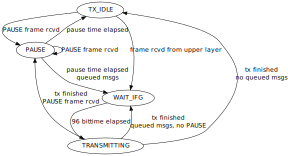
\includegraphics{figures/EtherMACFullDuplex_txstates}
\end{center}

The \nedtype{EtherMACFullDuplex} module records two scalars in addition to the
ones mentioned earlier:
\begin{itemize}
\item \ttt{rx channel idle (\%)}: reception channel idle time
        as a percentage of the total simulation time
\item \ttt{rx channel utilization (\%)}: total reception
        time as a percentage of the total simulation time
\end{itemize}

\subsection{EtherMAC}

Ethernet MAC layer implementing CSMA/CD. It supports both half-duplex and full-duplex operations;
in full-duplex mode it behaves as \nedtype{EtherMACFullDuplex}. In half-duplex  mode
it detects collisions, sends jam messages and retransmit frames upon collisions using
the exponential backoff algorithm. In Gigabit Ethernet networks it supports carrier
extension and frame bursting. Carrier extension can be turned off by setting the
\fpar{carrierExtension} parameter to \ttt{false}.

Unlike \nedtype{EtherMACFullDuplex}, this MAC module processes the incoming packets when their
first bit is received. The end of the reception is calculated by the MAC and
detected by scheduling a self message.

When frames collide the transmission is aborted -- in this case the transmitting
station transmits a jam signal. Jam signals are represented
by a \msgtype{EtherJam} message. The jam message contains the tree identifier
of the frame whose transmission is aborted. When the \nedtype{EtherMAC} receives a jam
signal, it knows that the corresponding transmission ended in jamming and have
been aborted. Thus when it receives as many jams as collided frames, it can
be sure that the channel is free again. (Receiving a jam message marks the
beginning of the jam signal, so actually has to wait for the duration of the jamming.)

The operation of the MAC module can be schematized by the following state chart:

\begin{center}
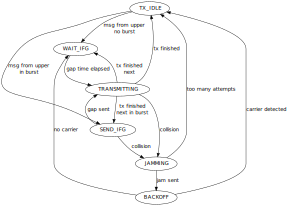
\includegraphics{figures/EtherMAC_txstates}
\end{center}

The module generates these extra signals:
\begin{itemize}
\item \fsignal{collision} when collision starts (received a frame,
         while transmitting or receiving another one; or start to transmit while receiving a frame),
         the constant value 1
\item \fsignal{backoff} when jamming period ended and before waiting according to the
         exponential backoff algorith, the constant value 1
\end{itemize}

These scalar statistics are generated about the state of the line:
\begin{itemize}
  \item \ttt{rx channel idle (\%)} reception channel idle time (full duplex) or channel
         idle time (half-duplex), as a percentage of the total simulation time
  \item \ttt{rx channel utilization (\%)} total successful reception time (full-duplex) or total
         successful reception/transmission time (half duplex), as a percentage
         of the total simulation time
  \item \ttt{rx channel collision (\%)} total unsuccessful reception time, as a percentage
         of the total simulation time
  \item \ttt{collisions} total number collisions (same as count of \fsignal{collisionSignal})
  \item \ttt{backoffs} total number of backoffs (same as count of \fsignal{backoffSignal})
\end{itemize}

% document error conditions (causing error() calls in the code)

% FIXME handleRestransmission() comment is not true: // no beginSendFrames(), because end of jam signal sending will trigger it automatically
%       in case of inner queue, the queued msg is not transmitted
% FIXME should not enter PAUSE state when !duplexMode


\section{Switches}

Ethernet switches play an important role in modern Ethernet LANs. Unlike
passive hubs and repeaters, that work in the physical layer, the switches
operate in the data link layer and routes data frames between the connected
subnets.

While a hub repeats the data frames on each connected line, possibly causing
collisions, switches help to segment the network to small collision domains.
In modern Gigabit LANs each node is connected to the switch direclty
by full-duplex lines, so no collisions are possible. In this case the
CSMA/CD is not needed and the channel utilization can be high.

\subsection{MAC relay units}

INET framework ethernet switches are built from \nedtype{IMACRelayUnit}
components. Each relay unit has N input and output gates for sending/receiving
Ethernet frames. They should be connected to \nedtype{IEtherMAC} modules.

Internally the relay unit holds a table for the destination address -> output
port mapping. When it receives a data frame it updates the table with the
source address->input port. The table can also be pre-loaded from a text file
while initializing the relay unit. The file name given as the \fpar{addressTableFile}
parameter. Each line of the file contains a hexadecimal MAC address and a decimal port
number separated by tabs. Comment lines beginning with '\#' are also allowed:

\begin{verbatim}
01 ff ff ff ff    0
00-ff-ff-ee-d1    1
0A:AA:BC:DE:FF    2
\end{verbatim}

% FIXME #352 addressTableSize is not checked in readAddressTable -> if overflown
%            then later check updateTableWithAddress has no effect
% FIXME format is wrong in the comment of readAddressTable()

The size of the lookup table is restricted by the \fpar{addressTableSize} parameter.
When the table is full, the oldest address is deleted. Entries are also deleted
if their age exceeds the duration given as the \fpar{agingTime} parameter.

If the destination address is not found in the table, the frame is broadcasted.
The frame is not sent to the same subnet it was received from, because the
target already received the original frame. The only exception if the frame
arrived through a radio channel, in this case the target can be out of range.
The port range 0..\fpar{numWirelessPorts}-1 are reserved for wireless connections.

The \nedtype{IMACRelayUnit} module is not a concrete implementation,
it just defines gates and parameters an \nedtype{IMACRelayUnit} should have.
Concrete inplementations add
capacity and performance aspects to the model (number of frames processed
per second, amount of memory available in the switch, etc.)
C++ implementations can subclass from the class \cppclass{MACRelayUnitBase}.

There are two versions of \nedtype{IMACRelayUnit}:

\begin{description}
  \item[\nedtype{MACRelayUnitNP}] models one or more CPUs with shared memory,
    working from a single shared queue.
  \item[\nedtype{MACRelayUnitPP}] models one CPU assigned to each incoming port,
    working with shared memory but separate queues.
\end{description}

In both models input messages are queued. CPUs poll messages from the queue
and process them in \fpar{processingTime}. If the memory usage exceeds
\fpar{bufferSize}, the frame will be dropped.

A simple scheme for sending PAUSE frames is built in (although
users will probably change it). When the buffer level goes
above a high watermark, PAUSE frames are sent on all ports.
The watermark and the pause time is configurable; use zero
values to disable the PAUSE feature.

% FIXME valid values for pauseTime: 0..0xFFFF
% FIXME ETHER_PAUSE_COMMAND_BYTES should be 4 in Ethernet.h (2bytes opcode + 2bytes pauseTime)
% FIXME PAUSE frame should not be sent on all ports probably
% TODO add lowWatermark, send PauseFrame(pauseUnits=0) to resume sending

The relay units collects the following statistics:

\begin{description}
\item[usedBufferBytes] memory usage as function of time
\item[processedBytes] count and length of processed frames
\item[droppedBytes] count and length of frames dropped caused by out of memory
\end{description}

% FIXME MACRelayUnitNP: no signals are generated, how does @statistic work in the ned file?

\subsection{EtherSwitch}

Model of an Ethernet switch containing a relay unit and multiple MAC units.

The duplexChannel attributes of the MACs must be set according to the
medium connected to the port; if collisions are possible (it's a bus or hub)
it must be set to false, otherwise it can be set to true.
By default it uses half duples MAC with CSMA/CD.

\begin{note}
Switches don't implement the Spanning Tree Protocol. You need to
avoid cycles in the LAN topology.
\end{note}

\section{Link Layer Control}
\label{sec:LLC}
% FIXME #353 there is no module for sending EtherFrameWithSNAP frames
% FIXME ETHER_SNAP_HEADER_LENGTH is wrong in Ethernet.h (+3 bytes, ssap+dsap+control)

\subsection{Frame types}

The raw 802.3 frame format header contains the MAC addresses of the destination and source
of the packet and the length of the data field. The frame footer contains the FCS
(Frame Check Sequence) field which is a 32-bit CRC.

\begin{center}
\begin{bytefield}[bitwidth=1.2em,bitheight=2\baselineskip]{20}
\bitbox{4}{\small MAC \\ destination} &
\bitbox{4}{\small MAC \\ source} &
\bitbox{4}{\small Length} &
\bitbox{4}{\small Payload} &
\bitbox{4}{\small FCS} \\
\bitbox{4}{\small 6 octets} &
\bitbox{4}{\small 6 octets} &
\bitbox{4}{\small 2 octets} &
\bitbox{4}{\small 46-1500 octets} &
\bitbox{4}{\small 4 octets}
\end{bytefield}
\end{center}

Each such frame is preceded by a 7 octet Preamble (with 10101010 octets) and
a 1 octet SFD (Start of Frame Delimiter) field (10101011) and followed by an
12 octet interframe gap. These fields are added and removed in the MAC layer,
so they are omitted here.

When multiple upper layer protocols use the same Ethernet line,
the kernel has to know which which component handles the incoming frames.
For this purpose a protocol identifier was added to the standard Ethernet
frames.

The first solution preceded the 802.3 standard and used a 2 byte protocol
identifier in place of the Length field. This is called Ethernet II
or DIX frame.
Each protocol id is above 1536, so the Ethernet II frames and the 802.3
frames can be distinguished.

\begin{center}
\begin{bytefield}[bitwidth=1.2em,bitheight=2\baselineskip]{20}
\bitbox{4}{\small MAC \\ destination} &
\bitbox{4}{\small MAC \\ source} &
\bitbox{4}{\small EtherType} &
\bitbox{4}{\small Payload} &
\bitbox{4}{\small FCS} \\
\bitbox{4}{\small 6 octets} &
\bitbox{4}{\small 6 octets} &
\bitbox{4}{\small 2 octets} &
\bitbox{4}{\small 46-1500 octets} &
\bitbox{4}{\small 4 octets}
\end{bytefield}
\end{center}

The LLC frame format uses a 1 byte source, a 1 byte destination, and a 1 byte
control information to identify the encapsulated protocol adopted from the
802.2 standard. These fields follow the standard 802.3 header, so the maximum
length of the payload is 1497 bytes:

\begin{center}
\begin{bytefield}[bitwidth=1.2em,bitheight=2\baselineskip]{20}
\bitbox{4}{\small MAC \\ destination} &
\bitbox{4}{\small MAC \\ source} &
\bitbox{4}{\small Length} &
\bitbox{4}{\small DSAP} &
\bitbox{4}{\small SSAP} &
\bitbox{4}{\small Control} &
\bitbox{4}{\small Payload} &
\bitbox{4}{\small FCS} \\
\bitbox{4}{\small 6 octets} &
\bitbox{4}{\small 6 octets} &
\bitbox{4}{\small 2 octets} &
\bitbox{4}{\small 1 octets} &
\bitbox{4}{\small 1 octets} &
\bitbox{4}{\small 1 octets} &
\bitbox{4}{\small 43-1497 octets} &
\bitbox{4}{\small 4 octets}
\end{bytefield}
\end{center}

The SNAP header uses the EtherType protocol identifiers inside an LLC header.
The SSAP and DSAP fields are filled with 0xAA (SAP\_SNAP), and the control
field is 0x03. They are followed by a 3 byte orgnaization and a 2 byte local
code the identify the protocol. If the organization code is 0, the local field
contains an EtherType protocol identifier.

\begin{center}
\begin{bytefield}[bitwidth=1.2em,bitheight=2\baselineskip]{20}
\bitbox{4}{\small MAC \\ destination} &
\bitbox{4}{\small MAC \\ source} &
\bitbox{4}{\small Length} &
\bitbox{4}{\small DSAP \\ 0xAA} &
\bitbox{4}{\small SSAP \\ 0xAA} &
\bitbox{4}{\small Control \\ 0x03} &
\bitbox{4}{\small OrgCode} &
\bitbox{4}{\small Local \\ Code} &
\bitbox{4}{\small Payload} &
\bitbox{4}{\small FCS} \\
\bitbox{4}{\small 6 octets} &
\bitbox{4}{\small 6 octets} &
\bitbox{4}{\small 2 octets} &
\bitbox{4}{\small 1 octets} &
\bitbox{4}{\small 1 octets} &
\bitbox{4}{\small 1 octets} &
\bitbox{4}{\small 3 octets} &
\bitbox{4}{\small 2 octets} &
\bitbox{4}{\small 38-1492 octets} &
\bitbox{4}{\small 4 octets}
\end{bytefield}
\end{center}

The INET defines these frames in the \ffilename{EtherFrame.msg} file.
The models supports Ethernet II, 803.2 with LLC header, and 803.3 with LLC and SNAP headers.
The corresponding classes are:
\msgtype{EthernetIIFrame}, \msgtype{EtherFrameWithLLC} and \msgtype{EtherFrameWithSNAP}. They all class
from \msgtype{EtherFrame} which only represents the basic MAC frame with source and
destination addresses. \nedtype{EtherMAC} only deals with \msgtype{EtherFrame}s, and does not
care about the specific subclass.

Ethernet frames carry data packets as encapsulated cMessage objects.
Data packets can be of any message type (cMessage or cMessage subclass).

The model encapsulates data packets in Ethernet frames using the \ttt{encapsulate()}
method of cMessage. Encapsulate() updates the length of the Ethernet frame too,
so the model doesn't have to take care of that.

The fields of the Ethernet header are passed in a \cppclass{Ieee802Ctrl}
control structure to the LLC by the network layer.


EtherJam, EtherPadding (interframe gap), EtherPauseFrame?


\subsection{EtherEncap}

The \nedtype{EtherEncap} module generates \msgtype{EthernetIIFrame} messages.

EtherFrameII

\subsection{EtherLLC}

EtherFrameWithLLC

SAP registration

% TODO delete EtherLLC, because LLC without SNAP is not used with IP (no ARP,IPv6 SAP)
% TODO modify EtherEncap to handle EtherFrameWithSNAP frames too (we can not send EtherFrameWithSNAP now)

\subsubsection{\nedtype{EtherLLC} and higher layers}

The \nedtype{EtherLLC} module can serve several applications (higher layer protocols),
and dispatch data to them. Higher layers are identified by DSAP.
See section "Application registration" for more info.

\nedtype{EtherEncap} doesn't have the functionality to dispatch to different
higher layers because in practice it'll always be used with IP.

\subsubsection{Communication between LLC and Higher Layers}

Higher layers (applications or protocols) talk to the \nedtype{EtherLLC} module.

When a higher layer wants to send a packet via Ethernet, it just
passes the data packet (a cMessage or any subclass) to \nedtype{EtherLLC}.
The message kind has to be set to IEEE802CTRL\_DATA.

In general, if \nedtype{EtherLLC} receives a packet from the higher layers,
it interprets the message kind as a command. The commands include
IEEE802CTRL\_DATA (send a frame), IEEE802CTRL\_REGISTER\_DSAP (register highher layer)
IEEE802CTRL\_DEREGISTER\_DSAP (deregister higher layer) and IEEE802CTRL\_SENDPAUSE
(send PAUSE frame) -- see EtherLLC for a more complete list.

The arguments to the command are NOT inside the data packet but
in a "control info" data structure of class \cppclass{Ieee802Ctrl}, attached to
the packet. See controlInfo() method of cMessage (OMNeT++ 3.0).

For example, to send a packet to a given MAC address and protocol
identifier, the application sets the data packet's message kind
to ETH\_DATA ("please send this data packet" command),
fills in the \nedtype{Ieee802Ctrl} structure with the destination MAC address and
the protocol identifier, adds the control info to the message, then sends
the packet to \nedtype{EtherLLC}.

When the command doesn't involve a data packet (e.g.
IEEE802CTRL\_(DE)REGISTER\_DSAP, IEEE802CTRL\_SENDPAUSE), a dummy packet
(empty cMessage) is used.

\subsubsection{Rationale}

The alternative of the above communications would be:

\begin{itemize}
  \item adding the parameters such as destination address into the data
    packet. This would be a poor solution since it would make the
    higher layers specific to the Ethernet model.
  \item encapsulating a data packet into an \textit{interface packet} which
    contains the destination address and other parameters. The
    disadvantages of this approach is the overhead associated with
    creating and destroying the interface packets.
\end{itemize}

Using a control structure is more efficient than the interface packet
approach, because the control structure can be created once inside
the higher layer and be reused for every packet.

It may also appear to be more intuitive in Tkenv because one can observe
data packets travelling between the higher layer and Ethernet
modules -- as opposed to "interface" packets.


\subsubsection{EtherLLC: SAP Registration}

The Ethernet model supports multiple applications or higher layer
protocols.

So that data arriving from the network can be dispatched to the
correct applications (higher layer protocols), applications
have to register themselves in \nedtype{EtherLLC}. The registration
is done with the IEEE802CTRL\_REGISTER\_DSAP command
(see section "Communication between LLC and higher layers")
which associates a SAP with the LLC port. Different applications
have to connect to different ports of \nedtype{EtherLLC}.

The ETHERCTRL\_REGISTER\_DSAP/IEEE802CTRL\_DEREGISTER\_DSAP commands use only the
dsap field in the \cppclass{Ieee802Ctrl} structure.

\subsection{EthernetInterface module}

The \nedtype{EthernetInterface} compound module implements the \nedtype{IWiredNic}
interface. Complements \nedtype{EtherMAC} and \nedtype{EtherEncap} with an output queue
for QoS and RED support. It also has configurable input/output filters as \nedtype{IHook}
components similarly to the \nedtype{PPPInterface} module.

% TODO there is no IWiredNic with EtherLLC

\section{Ethernet applications}

The \nedtype{inet.applications.ethernet} package contains modules
for a simple client-server application. The \nedtype{EtherAppCli} is a simple
traffic generator that peridically sends \msgtype{EtherAppReq} messages
whose length can be configured. destAddress, startTime,waitType, reqLength, respLength

The server component of the model (\nedtype{EtherAppSrv}) responds with a
\msgtype{EtherAppResp} message of the requested length. If the response does
not fit into one ethernet frame, the client receives the data in multiple
chunks.

% FIXME reqLength>1500 causes an error in the LLC module
% FIXME numFrames field of EtherAppRes is not used
% FIXME server always sends 1497 byte chunks, it should depend on the framing (1497 is for LLC)
% FIXME if registerSAP is false (default), the and EtherLLC used, then the client won't receive messages (auto config?)
% FIXME Ieee802Nic -> EthernetInterface in the NED comment

Both applications have a \fpar{registerSAP} boolean parameter.
This parameter should be set to \ttt{true} if the application is connected
to the \nedtype{EtherLLC} module which requires registration of the SAP
before sending frames.

Both applications collects the following statistics: sentPkBytes, rcvdPkBytes,
endToEndDelay.

The client and server application works with any model that accepts
Ieee802Ctrl control info on the packets (e.g. the 802.11 model).
The applications should be connected directly to the \nedtype{EtherLLC}
or an EthernetInterface NIC module.

The model also contains a host component that groups the applications
and the LLC and MAC components together (\nedtype{EtherHost}). This node does
not contain higher layer protocols, it generates Ethernet traffic directly.
By default it is configured to use half duplex MAC (CSMA/CD).

\section{Ethernet networks}

\subsection{\nedtype{LargeNet} model}

The \nedtype{LargeNet} model demonstrates how one can put together models of large
LANs with little effort, making use of MAC auto-configuration.

\nedtype{LargeNet} models a large Ethernet campus backbone. As configured in the
default omnetpp.ini, it contains altogether about 8000 computers
and 900 switches and hubs. This results in about 165MB process size
on my (32-bit) linux box when I run the simulation.
The model mixes all kinds of Ethernet technology: Gigabit Ethernet,
100Mb full duplex, 100Mb half duplex, 10Mb UTP, 10Mb bus ("thin Ethernet"),
switched hubs, repeating hubs.

The topology is in \nedtype{LargeNet}.ned, and it looks like this: there's chain
of n=15 large "backbone" switches (switchBB[]) as well as four more
large switches (switchA, switchB, switchC, switchD) connected to
somewhere the middle of the backbone (switchBB[4]). These 15+4 switches
make up the backbone; the n=15 number is configurable in omnetpp.ini.

Then there're several smaller LANs hanging off each backbone switch.
There're three types of LANs: small, medium and large (represented by
compound module types \nedtype{SmallLAN}, \nedtype{MediumLAN}, \nedtype{LargeLAN}). A small LAN
consists of a few computers on a hub (100Mb half duplex); a medium
LAN consists of a smaller switch with a hub on one of its port
(and computers on both); the large one also has a switch and a hub,
plus an Ethernet bus hanging of one port of the hub (there's still hubs
around with one BNC connector besides the UTP ones).
By default there're 5..15 LANs of each type hanging off each backbone
switch. (These numbers are also omnetpp.ini parameters like the length
of the backbone.)

The application model which generates load on the simulated LAN is
simple yet powerful. It can be used as a rough model for any
request-response based protocol such as SMB/CIFS (the Windows file
sharing protocol), HTTP, or a database client-server protocol.

Every computer runs a client application (\nedtype{EtherAppCli}) which connects
to one of the servers. There's one server attached to switches A, B,
C and D each: serverA, serverB, serverC and serverD -- server selection
is configured in omnetpp.ini). The servers run \nedtype{EtherAppSrv}.
Clients periodically send a request to the server, and the request
packet contains how many bytes the client wants the server to send back
(this can mean one or more Ethernet frames, depending on the byte count).
 Currently the request and reply lengths are configured in omnetpp.ini
as intuniform(50,1400) and truncnormal(5000,5000).

The volume of the traffic can most easily be controlled with the
time period between sending requests; this is currently
set in omnetpp.ini to exponential(0.50) (that is, average 2
requests per second). This already causes frames to be dropped
in some of the backbone switches, so the network is a bit
overloaded with the current settings.

The model generates extensive statistics. All MACs (and most other
modules too) write statistics into omnetpp.sca at the end
of the simulation: number of frames sent, received, dropped, etc.
These are only basic statistics, however it still makes the
scalar file to be several ten megabytes in size. You can use
the analysis tools provided with OMNeT++ to visualized the data
in this file. (If the file size is too big, writing statistics
can be disabled, by putting **.record-scalar=false in the ini file.)
The model can also record output vectors, but this is currently
disabled in omnetpp.ini because the generated file can easily reach
gigabyte sizes.

%%% Local Variables:
%%% mode: latex
%%% TeX-master: "usman"
%%% End:

\cleardoublepage

\ifdraft TODO

\chapter{The Physical Environment}
\label{cha:environment}

TODO C++ interface

\fi



\cleardoublepage

\chapter{Modeling Power Consumption}
\label{cha:power}

\section{Overview}
\label{sec:power:overview}

Modeling power consumption becomes more and more important with the increasing
number of embedded devices and the upcoming Internet of Things. Mobile personal
medical devices, large scale wireless environment monitoring devices, electric
vehicles, solar panels, low-power wireless sensors, etc. require paying special
attention to power consumption. The high fidelity simulation of power
consumption allows designing power sensitive routing protocols, MAC protocols,
physical layers, etc. which in turn results in more energy efficient devices.

In order to help the modeling process the power model is separated from other
simulation models. This separation makes the model extensible and it also allows
easy experimentation with alternative implementations. In a nutshell the power
model consists of the following components:

\begin{itemize}
  \item energy consumption models
  \item energy generation models
  \item temporary energy storage models
\end{itemize}

The power model elements fall into two categories, abbreviated with \ttt{Ep}
and \ttt{Cc} as part of their names:

\begin{itemize}
  \item \ttt{Ep} models are simpler, and deal with energy and power quantities.
  \item \ttt{Cc} models are more realistic, and deal with charge, current, and voltage quantities.
\end{itemize}

The following sections provide a brief overview of the power model.

\section{Energy Consumer Models}
\label{sec:power:energy-consumer-models}

Energy consumer models describe the energy consumption of devices over time.
For example, a transceiver consumes energy when it transmits or
receives signals, a CPU consumes energy when the network protocol routes
packets, and a display consumes energy when it's turned on.

In INET, an energy consumer model is an OMNeT++ simple module that implements
the energy consumption of software processes or hardware devices over time.
Its main purpose is to provide the power or current consumption for the
current simulation time. Most often energy consumers are included as
submodules in the compound module of the hardware devices or software
components.

INET provides only a few built-in energy consumer models:

\begin{itemize}
        \item \nedtype{AlternatingEpEnergyGenerator} is a trivial energy/power based statistical energy consumer model example.
        \item \nedtype{StateBasedEpEnergyConsumer} is a transceiver energy consumer model based on the radio mode and transmission/reception states.
\end{itemize}

In order to simulate power consumption in a wireless network, the energy
consumer model type must be configured for the transceivers. The following
example demonstrates how to configure the power consumption parameters for
a transceiver energy consumer model:

\inisnippet{EnergyConsumerConfigurationExample}{Energy consumer configuration example}


\section{Energy Generator Models}
\label{sec:power:energy-generator-models}

Energy generator models describe the energy generation of devices over time.
A solar panel, for example, produces energy based on time, the panel's
position on the globe, its orientation towards the sun and the actual weather
conditions. Energy generators connect to an energy storage that absorbs the
generated energy.

In INET, an energy generator model is an OMNeT++ simple module implementing
the energy generation of a hardware device using a physical phenomena over
time. Its main purpose is to provide the power or current generation for
the current simulation time. Most often energy generation models are
included as submodules in network nodes.

INET provides only one trivial energy/power based statistical energy
generator model called \nedtype{AlternatingEpEnergyGenerator}. The following
example shows how to configure its power generation parameters:

\inisnippet{EnergyGeneratorConfigurationExample}{Energy generator configuration example}

\section{Energy Storage Models}
\label{sec:power:energy-storage-models}

Electronic devices which are not connected to external power source must contain
some component to store energy. For example, an electrochemical battery in a
mobile phone provides energy for its display, its CPU, and its communication
devices. It might also absorb energy produced by a solar installed on its
display, or by a portable charger plugged into the wall socket.

In INET, an energy storage model is an OMNeT++ simple module which models
the physical phenomena that is used to store energy produced by generators
and provide energy for consumers. Its main purpose is to compute the amount
of available energy or charge at the current simulation time. It maintains
a set of connected energy consumers and energy generators, their respective
total power consumption and total power generation.

INET contains a few built-in energy storage models:

\begin{itemize}
        \item \nedtype{IdealEpEnergyStorage} is an idealistic model with infinite energy capacity and infinite power flow.
        \item \nedtype{SimpleEpEnergyStorage} is a non-trivial model integrating the difference between the total consumed power and the total generated power over time.
        \item \nedtype{SimpleCcBattery} is a more realistic charge/current based battery model using a charge independent ideal voltage source and internal resistance.
\end{itemize}

The following example shows how to configure a simple energy storage model:

\inisnippet{EnergyStorageConfigurationExample}{Energy storage configuration example}

\section{Energy Management Models}
\label{sec:power:energy-management-models}

% Why energy management models are needed?
% The energy management models monitors an energy storage, estimates its state, and controls the consumers and generators to protect the energy storage from operating outside its safe operating area.

\nedtype{SimpleEpEnergyManagement}

\inisnippet{EnergyManagementConfigurationExample}{Energy management configuration example}



%%% Local Variables:
%%% mode: latex
%%% TeX-master: "usman"
%%% End:


\cleardoublepage

\ifdraft TODO

\chapter{The Physical Layer}
\label{cha:physicallayer}

TODO which modules? C++ interface

\begin{itemize}
  \item ongoing transmissions
  \item recent successful receptions
  \item recent obstacle intersections and surface normal vectors
\end{itemize}

\begin{verbatim}
TODO: 
 - exploit multiple CPUs and the highly parallel GPU to increase performance
 - provide performance vs. accuracy tradeoff configuration options
   (e.g. range filter, radio mode filter, listening mode filter, MAC address filter)
 - support different level of details (see details below)
 - support different transmitters and receivers (scale from flat to layered models)
 - support different radio signal models (scale from range based to accurate emulation models)
 - support different propagation models (scale from immediate to accurate models)
 - support different attenuation models (scale from free space to trace based models)
 - support different antenna models (scale from isotropic to directional models)
 - support different power consumption models (scale from mode based to signal based models)
 - provide concurrent transmitter and receiver mode (transceiver mode)
 - provide burst mode (back to back) transmissions
 - provide synchronization/preamble detection
 - provide capture during reception (switching to another transmission)
 - provide finite time radio mode switching

TODO: scalar vs dimensional
TODO: flat vs layered
TODO: Generic, IEEE 802.11, IEEE 802.15.4
TODO: acoustic underwater example
TODO: wireless vs. wired medium

\end{verbatim}

\section{Overview}

Today's electric devices use more and more wireless communication methods such
as Wifi, Bluetooth, NFC, UMTS, and LTE. Despite the diversity of these devices
there are many similarities in the modeling of their physical layer components.
The models often have similar signal representations and signal processing steps,
and they also share the physical medium model where communication takes place.

In general, the physical layer simulation is a very time consuming task. The
simulation of signal propagation, signal fading, signal interference, and signal
decoding in detail may often result in unacceptable performance. Finding the
right abstractions, the right level of detail, and the right trade-offs between
accuracy and performance is difficult and very important.

To summarize, the physical layer is designed with the following goals in mind:
\begin{itemize}
  \item customizability
  \item extensibility
  \item scalable level of detail
  \item ability to exploit parallel hardware
\end{itemize}

The following sections provide a brief overview of the physical layer model. For
more details on the available modules, their parameterization and the actual
implementations please refer to the documentation in the corresponding NED and
C++ source files.

\subsection{Customizability}

Real world communication devices often provide a wide variety of configuration
options to allow adapting to the physical conditions where they are required
to operate. For example, a Wifi router administration interface often provides
parameters to configure the transmission power, bitrate, preamble type, carrier
frequency, RTS threshold, beacon interval, etc. Mostly these parameters have
default values assigned, so the user doesn't have to set them separately, but
may override them as needed.

Similarly to real world devices the physical layer models also provide a wide
variety of parameters to control their behavior. The most common NED parameters
are various physical quantities with physical units such as transmission power
\ttt{[W]}, reception sensitivity \ttt{[W]}, carrier frequency \ttt{[Hz]},
communication range \ttt{[m]}, propagation speed \ttt{[m/s]}, SNIR reception
threshold \ttt{[dB]}, bitrate \ttt{[b/s]}. Occasionally models support new
parameters or new combinations, which don't exist in real world hardware, to
allow further experimentation.

Another important and commonly used parameter kind selects among alternative
implementations of a particular interface by providing its name. Different
implementations are often separate modules, which come with their own set of
parameters to avoid the confusion of mixing their unrelated parameters. Some
modules may be split into more submodules. This further deepens the module
hierarchy, but allows better extensibility.

\subsection{Extensibility}

Similarly to designing other simulation models, modeling the physical layer is
not at all an unambiguous task. For example, the research literature contains a
number of different path loss models for signal propagation, there are different
bit error models for a particular protocol standard, representing the signal in
the analog domain can also be done in several different ways, and so on.

In order to support this diversity the physical layer is designed to be
extensible with alternative implementations at various parts of the model. This
is realized by separately defining C++ and NED interfaces between modules, and
also by providing parameters in their parent modules to easily select among the
available implementations.

New models can be added by implementing the required interfaces from scratch, or
by deriving from already existing implementations and overriding functionality.
This architecture allows the user to create new models with less effort, and to
focus on the real differences, while the rest of the physical layer remains the
same.

\subsection{Scalable Level of Detail}

There are many possible ways to model various aspects of the physical layer.
The most important difference lies in the trade-off between performance versus
accuracy. In order to support the different trade-offs the physical layer is
designed to be scalable with respect to the simulated level of detail. In other
words, it's scalable from high-performance less accurate simulations to high
fidelity slower simulations.

The physical layer model is scalable along the following axes:

\begin{itemize}
  \item simulation model -- statistical vs accurate
  \item software architecture -- flat vs layered
  \item data representation -- scalar vs multi-dimensional
  \item number of messages -- TODO 
\end{itemize}

The simulation model might vary from simple statistical models to accurate
emulation. The simplest models ignore the actual bits of the transmission. For
example, the extremely simple unit disc radio even ignores the signal power. The
most accurate models use precise signal representation for all four domains:
bit domain, symbol domain, sample domain, and analog domain representations.
They also emulate most functions of real hardware in detail: forward error
correction, interleaving, scrambling, modulation, spreading, pulse shaping, and
so on.

The software architecture might vary from flat to layered. A flat architecture
is efficient but not modular. Functionality can only be affected through simple
parameters and not by providing alternative implementations. Whereas a layered
architecture is more flexible at the cost of more complex data structures, more
data conversions, more resource management, and thus slower processing. On the
other hand, it provides more customization opportunities to replace parts with
alternative implementations and to do research easier in the area.

The data representation might vary from scalar to multidimensional values. In
the analog domain of the physical layer data quite often changes over time,
frequency, space, or any combination thereof. The most obvious example is the
analog signal power, but there are others such as signal phase or the signal to
noise ratio.

The number of messages per transmission added to the future event queue might
vary from one to the number of radios. One message might be sufficient, for
example, if the transmission is intended to a single destination, and other
receivers are either not affected, or the effect is negligible. On the other
hand, it might be necessary to process all transmissions by all receivers in
order to have the desired effect on the higher layers. For example, if a MAC
model is configured to promiscuous mode, it needs to receive all transmissions.

\subsection{Exploiting Parallel Hardware}

The physical processes simulated by the physical layer are inherently parallel.
The computation of the transmission arrival space-time coordinates, the analog
signal representation of transmissions and receptions, the interfering
receptions and noises, the signal to noise ratio, the decoded bits, the bit
errors, and the physical layer indications all provide a good parallelization
opportunity, because they dominate the physical layer performance and are
independent for each receiver. Therefore the physical layer is designed to be
able to utilize parallel hardware, multi-core CPUs, vector instructions and the
highly parallel GPU.

The idea is to have a central component in the software architecture where
parallel computation can happen. This central component is the medium model
that knows about all radios, transmissions, interferences, and receptions
anyway. It uses optimistic parallel computation in multiple background threads
while the main simulation thread continues normal execution. When a new
transmission enters the channel the already computed and affected results are
invalidated or updated, and the affected ongoing optimistic parallel
computations are canceled.

\section{The Radio Model}

The radio model describes the physical device that is capable of transmitting
and receiving signals on the medium. It contains an antenna model, a transmitter
model, a receiver model, and an energy consumer model. The antenna model is
shared between the transmitter model and the receiver model. The separation of
the transmitter model and the receiver model allows asymmetric configurations.
The energy consumer model is optional and it's only used when the simulation of
energy consumption is necessary.

The radio model has an operational mode that is called the radio mode. The radio
mode is externally controlled usually by the MAC model. In transceiver mode, the
radio can simultaneously transmit and receive a signal. Changing the radio mode
may optionally take a non-zero amount of time. The supported radio modes are the
following:

\begin{itemize}
  \item \ttt{off}: communication isn't possible, energy consumption is zero
  \item \ttt{sleep}: communication isn't possible, energy consumption is minimal
  \item \ttt{receiver}: only reception is possible, energy consumption is low
  \item \ttt{transmitter}: only transmission is possible, energy consumption is
high
  \item \ttt{transceiver}: reception and transmission is simultaneously
possible, energy consumption is high
  \item \ttt{switching}: communication isn't possible, energy consumption is
minimal
\end{itemize}

In addition to the radio mode, the transmitter and the receiver models have
separate states which describe what they are doing. Changes to these states are
automatically published by the radio. The signaled transmitter states are the
following:

\begin{itemize}
  \item \ttt{undefined}: isn't operating
  \item \ttt{idle}: there's no transmission in progress
  \item \ttt{transmitting}: transmission is in progress
\end{itemize}

The signaled receiver states are the following:

\begin{itemize}
  \item \ttt{undefined}: isn't operating
  \item \ttt{idle}: there's no reception in progress
  \item \ttt{busy}: received signal is not interpretable
  \item \ttt{synchronizing}: synchronization is in progress
  \item \ttt{receiving}: reception is in progress
\end{itemize}

When a radio wants to transmit a signal on the medium it sends direct messages
to all affected radios with the help of the central medium module. The messages
contain a shared data structure which describes the transmission the way it
entered the medium. The messages arrive at the moment when start of the
transmission arrive at the receiver. The receiver radios also handle the
incoming messages with the help of the central medium module. This kind of
centralization allows the medium to do shared computations in a more efficient
way and it also makes parallel computation possible.

As stated above the radio module utilizes multiple submodules to further split
its task. This design decision makes it more extensible and customizable. The
following sections describe the parts of the radio model.

\subsection{Antenna Models}

The antenna model describes the effects of the physical device which converts
electric signals into radio waves, and vice versa. This model captures the
antenna characteristics that heavily affect the quality of the communication
channel. For example, various antenna shapes, antenna size and geometry, antenna
arrays, and antenna orientation causes different directional or frequency
selectivity.

The antenna model provides a position and an orientation using a mobility model
that defaults to the mobility of the node. The main purpose of this model is to
compute the antenna gain based on the specific antenna characteristics and the
direction of the signal. The signal direction is computed by the medium from the
position and the orientation of the transmitter and the receiver. The following
list provides some examples:

\begin{itemize}
  \item \nedtype{IsotropicAntenna}: antenna gain is exactly 1 in any direction
  \item \nedtype{ConstantGainAntenna}: antenna gain is a constant determined by
a parameter
  \item \nedtype{DipoleAntenna}: antenna gain depends on the direction according
to the dipole antenna characteristics
  \item \nedtype{InterpolatingAntenna}: antenna gain is computed by linear
interpolation according to a table indexed by the direction angles
\end{itemize}

The antenna models are in the \ttt{src/physicallayer/antenna/} directory.

\subsection{Transmitter Models}

The transmitter model describes the physical process which converts packets into
electric signals. In other words, this model converts a MAC packet into a signal
that is transmitted on the medium. The conversion process and the representation
of the signal depends on the level of detail and the physical characteristics
of the implemented protocol.

In the flat model the transmitter model skips the symbol domain and the sample
domain representations, and it directly creates the analog domain representation.
The bit domain representation is reduced to the bit length of the packet and the
actual bits are ignored.

In the layered model the conversion process involves various processing steps
such as packet serialization, forward error correction encoding, scrambling,
interleaving, and modulation. This transmitter model requires much more
computation, but it produces accurate bit domain, symbol domain, and sample
domain representations.

The various protocol specific transmitter models are in the corresponding
directories.

\subsection{Receiver Models}

The receiver model describes the physical process which converts electric
signals into packets. In other words, this model converts a reception, along
with an interference computed by the medium model, into a MAC packet and a
reception indication. It also determines the following for each transmission: 

\begin{itemize}
  \item \ttt{is the reception possible or not}: based on the signal
characteristics such as reception power, carrier frequency, bandwidth, preamble
mode, modulation scheme
  \item \ttt{if the reception is possible, is reception attempted or not}: based
on the ongoing reception and the support of signal capturing
  \item \ttt{if the reception is attempted, is reception successful or not}:
based on the error model and the simulated part of the signal decoding
\end{itemize}

In the flat model the receiver model skips the sample domain, the symbol domain,
and the bit domain representations, and it directly creates the packet domain
representation by copying the packet from the transmission. It uses the error
model to decide if the reception is successful or not.

In the layered model the conversion process involves various processing steps
such as demodulation, descrambling, deinterleaving, forward error correction
decoding, and deserialization. This reception model requires much more
computation, but it produces accurate sample domain, symbol domain, and bit
domain representations.

The various protocol specific receiver models are in the corresponding 
directories.

\subsection{Transmission Error Modeling}

Determining the reception errors is a crucial part of the reception process.
There are often several different statistical error models in the literature
even for a particular physical layer. In order to support this diversity the
error model is a separate replaceable component of the receiver. 

The error model describes how the signal to noise ratio affects the amount of
errors at the receiver. The main purpose of this model is to determine whether
if the received packet has errors or not. It also computes various physical
layer indications for higher layers such as packet error rate, bit error rate,
and symbol error rate. For the layered reception model it needs to compute the
erroneous bits, symbols, or samples depending on the lowest simulated physical
domain where the real decoding starts. The error model is optional, if omitted
all receptions are considered successful.

The error models are in the \ttt{src/physicallayer/errormodel/} directory and
also in the corresponding protocol specific directories.

\subsection{Power Consumption Models}

A substantial part of the energy consumption of communication devices comes from
transmitting and receiving signals. The energy consumer model describes how the
radio consumes energy depending on its activity. This model is optional, if
omitted energy consumption is ignored. The following list provides some examples:

\begin{itemize}
  \item \nedtype{StateBasedEnergyConsumer}: the constant power consumption is
determined by valid combinations of the radio mode, the transmitter state and
the receiver state
\end{itemize}

The energy consumer models are in the \ttt{src/physicallayer/energyconsumer/} directory.

TODO: layered

This module further splits the transmitter and receiver models to allow bit
precise communication modeling.

TODO: layered

The following sections describe the parts of the layered radio model.

\subsubsection{Encoding and Decoding}

This module describes how the packet domain signal representation is converted
into the bit domain, and vice versa.

TODO: layered

\subsubsection{Modulation and Demodulation}

This module describes how the bit domain signal representation is converted into
the symbol domain, and vice versa.

TODO: layered

\subsubsection{Pulse Shaping and Pulse Filtering}

This module describes how the symbol domain signal representation is converted
into the sample domain, and vice versa.

TODO: layered


\subsubsection{Digital Analog and Analog Digital Conversion}

This module describes how the sample domain signal representation is converted
into the analog domain, and vice versa.

TODO: layered

\section{The Medium Model}

The medium model describes the shared physical medium where communication takes
place. It keeps track of radios, noise sources, ongoing transmissions,
background noise, and other ongoing noises. The medium computes when, where and
how transmissions and noises arrive at receivers. It also efficiently provides
the set of interfering transmissions and noises for the receivers. It doesn't
send or handle messages on its own, it rather acts as a mediator between radios.

The medium model has a separate chapter devoted to it, see \ref{cha:transmission-medium}. 

\section{Signal Representation}

The data structures that represent the transmitted and the received signals
might contain many different data depending on the simulated level of detail. In
addition, the reception data structure might contain various physical layer
indications, which are computed during the reception process. The following list
provides some examples:

\begin{itemize}
  \item \ttt{packet domain}: actual packet, packet error rate, packet error bit,
etc.
  \item \ttt{bit domain}: various bit lengths, bitrates, actual bits, forward
error correction code, interleaving scheme, scrambling scheme, bit error rate,
number of bit errors, actual erroneous bits, etc.
  \item \ttt{symbol domain}: number of symbols, symbol rate, actual symbols,
modulation scheme, symbol error rate, number of symbol errors, actual erroneous
symbols, etc.
  \item \ttt{sample domain}: number of samples, sampling rate, actual samples,
etc.
  \item \ttt{analog domain}: space-time coordinates, antenna orientations,
communication range, interference range, detection range, carrier frequency,
subcarrier frequencies, bandwidths, scalar or dimensional power, receive signal
strength indication, signal to noise and interference ratio, etc.
\end{itemize}

In simple case the packet domain specifies the MAC packet only, and the bit
domain specifies the bit length and the bitrate. The symbol domain specifies the
used modulation, and the sample domain is simply ignored. The most important
part is the analog domain representation, because it's indispensable to be able
to compute some kind of signal to noise and interference ratio. The following
figure shows four different kinds of analog domain representations, but other
representations are also possible.

\begin{figure}[h!]
\centering
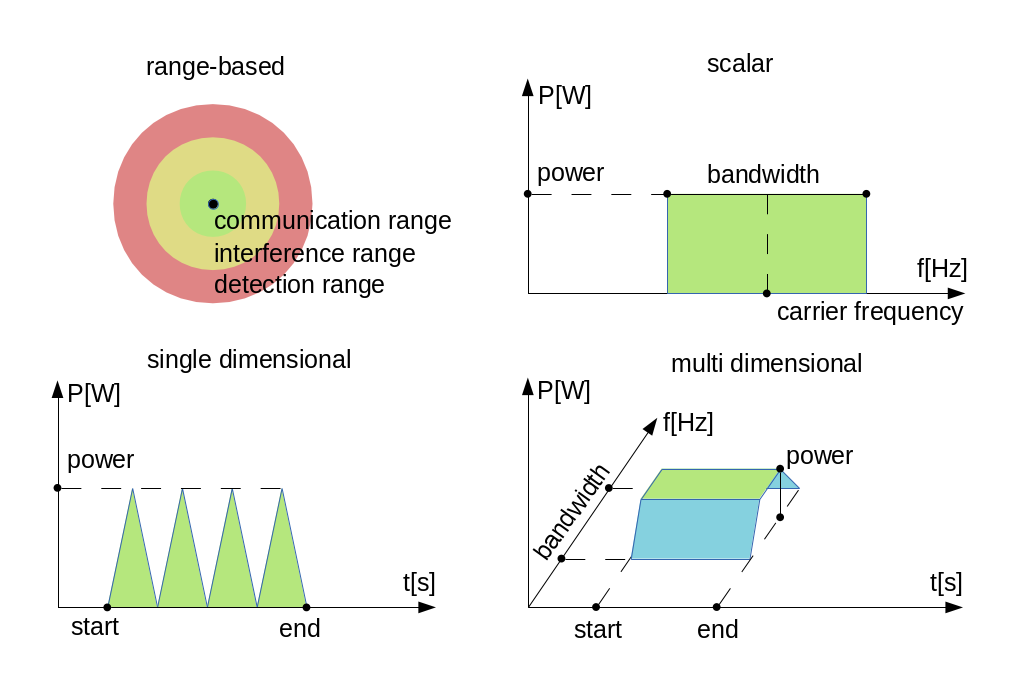
\includegraphics[width=\textwidth]{figures/phyanalog}
\caption{Various analog signal representations}
\end{figure}

The first representation is called range-based, and it's used by the unit disc
radio. The advantage of this data structure is that it's compact, predictable,
and provides high performance. The disadvantage is that it's very inaccurate in
terms of modeling reality. Nevertheless, this representation might be sufficient
for developing a new routing protocol if accurate simulation of packet loss is
not important.

The second data structure represents a narrowband signal with a scalar signal
power, a carrier frequency, and a bandwidth. The advantage of this
representation is that it allows to compute a real signal to noise ratio, which
in turn can be used by the error model to compute bit and packet error rates.
This representation is most of the time sufficient for the simulation of IEEE
802.11 networks.

The third data structure describes a signal power that changes over time. In
this case the signal power is represented with a one-dimensional time dependent
value that precisely follows the transmitted pulses. This representation is used
by the IEEE 802.15.4a UWB radio.

The last representation uses a multi-dimensional value to describe the signal
power that changes over both time and frequency. The IEEE 802.11b model might
use this representation to simulate crosstalk, where one channel interferes with
another. In order to make it work the frequency spectrum of the signal has to
follow the real spectrum more precisely at both ends of the band.

The flat signal representation uses a single object to simulatenously describe
all domains of the transmission or the reception. In contrast, the layered
signal representation uses one object to describe every domain seperately. The
advantage of the latter is that it's extensible with alternative implementations
for each domain. The disadvantage is that it needs more allocation and resource
management.

\section{Signal Processing}

The following figure shows the process of how a MAC packet gets from the
transmitter radio through the medium to the receiver radio. The figure focues on
how data flows between the processing components of the physical layer. The blue
boxes represent the data structures, and the red boxes represent the processing
components.

\begin{figure}[h!]
\centering
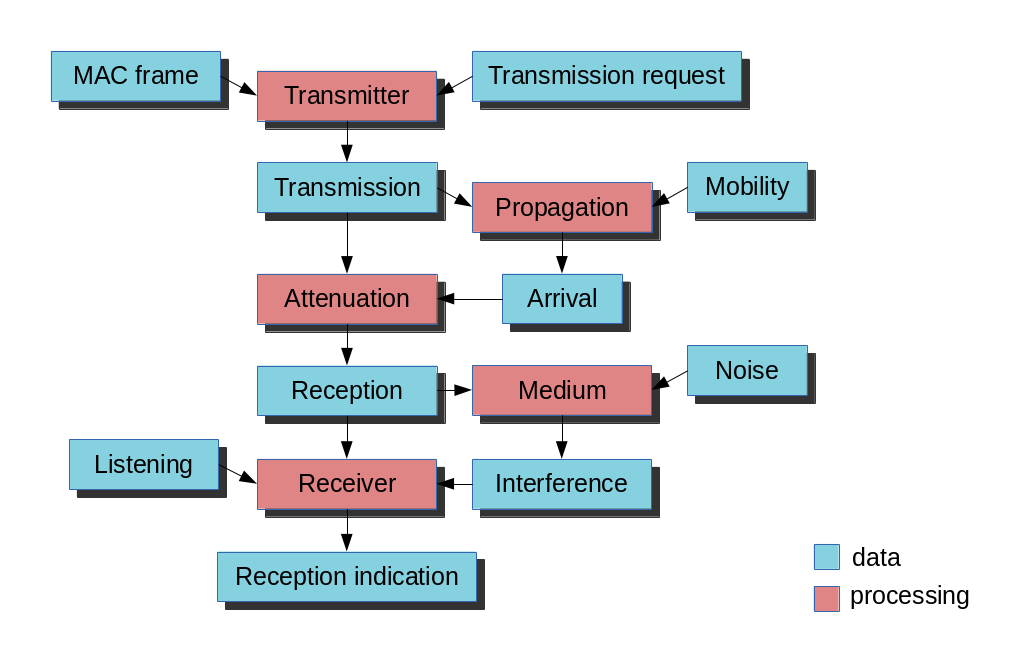
\includegraphics[width=\textwidth]{figures/phydataflow}
\caption{Signal processing data flow}
\end{figure}

The transmission process starts in the transmitter radio when it receives a MAC
packet from the higher layer. The radio must be in transmitter or transceiver
mode before receiving a MAC packet, otherwise it throws an exception. At first
the transmitter model creates a data structure that describes the transmitted
signal based on the received MAC packet and the attached transmission request.
The resulting data structure is immutable, it's not going to be changed in any
later processing step.

Thereafter the propagation model computes the arrival space-time coordinates for
all receivers. In the next step the medium model determines the set of affected
receivers. Which radio constitutes affected depends on a number of factors such
as the maximum communication range of the transmitter, the radio mode of the
receiver, the listening mode of the receiver, or potentially the MAC address of
the receiver. Using the result the medium model sends a separate message with
the shared transmission data structure to all affected receivers. There's no
need to send a message to all radios on the channel, because the computation
of interfering signals is independent of this step.

Thereafter the attenuation model computes the reception for the receiver using
the original transmission and the arrival data structure. It applies the path
loss model, the obstacle loss model and the multipath model to the transmission.
The resulting data structure is also immutable, it's not going to be changed in
any later processing step.

Thereafter the medium model computes the interference for the reception by
collecting all interfering receptions and noises. Another signal is considered
interfering if it owerlaps both in time and frequency domains with respect to 
the minimum interference parameters. The background noise model also computes a 
noise signal that is added to the interference.

The reception process starts in the receiver radio when it receives a message
from the transmitter radio. The radio must be in receiver or transceiver mode
before the message arrives, otherwise it ignores the message. At first the
receiver model determines is whether the reception is actually attempted or not.
This decision depends on the reception power, whether there's another ongoing
reception process, and capturing is enabled or not.

Thereafter the receiver model computes the signal to noise and interference
ratio from the reception and the interference. Using the result, the bitrate,
and the modulation scheme the error model computes the necessary error rates.
Alternatively the error model might compute the erroneous bits, or symbols by
altering the corresponding data of the original transmission. 

Thereafter the receiver determines the received MAC packet by either simply
reusing the original, or actually decoding from the lowest represented domain
in the reception. Finally, it attaches the physical layer indication to the MAC
packet, and sends it up to the higher layer.

The following sections describe the data structures that are created during
signal processing.

\subsubsection{Transmission Request}

This data structure contains parameters that control how the transmitter
produces the transmission. For example, it might override the default
transmission power, ot the default bitrate of the transmitter. It is attached as
a control info object to the MAC packet sent down from the MAC module to the
radio.

\subsubsection{Transmission}

This data structure describes the transmission of a signal. It specifies the
start/end time, start/end antenna position, start/end antenna orientation of the
transmitter. In other words, it describes when, where and how the signal
started/ended to interact with the medium. The transmitter model creates one
transmission instance per MAC packet.

\subsubsection{Arrival}

This data structure decscirbes the space and time coordinates of a transmission
arriving at a particular receiver. It specifies the start/end time, start/end
antenna position, start/end antenna orientation of the receiver. The propagation
model creates one arrival instance per transmission per receiver.

\subsubsection{Listening}

This data structure describes the way the receiver radio is listening on the
medium. The physical layer ignores certain transmissions either during computing
the interference or even the complete reception of such transmissions. For
example, a narrowband listening specifies a carrier frequency and a bandwidth. 

\subsubsection{Reception}

This data structure describes the reception of a signal by a particular receiver.
It specifies at least the start/end time, start/end antenna position, start/end
antenna orientation of the receiver. The attenuation model creates one reception
instance per transmission per receiver.

\subsubsection{Noise}

This data structure describes a meaningless signal or a meaningless composition
of multiple signals. All models contain at least the start/end time, and
start/end position.

\subsubsection{Interference}

This data structure describes the interfering signals and noises that affect a
particular reception. It also specifies the total noise that is the composition
of all interference.

\subsubsection{SNIR}

This data structure describes the signal to noise and interference ratio of a
particular reception. It also specifies the minimum signal to noise and
interference ratio.

\subsubsection{Reception Decision}

This data structure describes whether if the reception of a signal is possible
or not, is attempted or not, and is successful or not.

\subsubsection{Reception Indication}

This data structure describes the physical layer indications such as RSSI, SNIR,
PER, BER, SER. These physical properties are optional and may be omitted if the
receiver is configured to do so or if it doesn't support providing the data. The
reception indication is attached as a control info object to the MAC packet sent
up from the radio to the MAC module. 

\section{Visualization}

In order to help understanding the communication in the network the physical
layer supports visualizing its state. The following list shows what can be
displayed:

\begin{itemize}
  \item ongoing transmissions
  \item recent successful receptions
  \item recent obstacle intersections and surface normal vectors
\end{itemize}

The ongoing transmissions can be displayed with 3 dimensional spheres or with 2
dimensional rings laying in the XY plane. As the signal propagates through space
the figure grows with it to show where the beginning of the signal is. The inner
circle of the ring figure shows as the end of the signal propagates through
space. 

The recent successful receptions are displayed as straight lines between the
original positions of the transmission and the reception. The recent obstacle
intersections are also displayed as straight lines from the start of the
intersection to the end of it.

\section{TODO other stuff}

TODO: scalar vs dimensional

TODO: flat vs layered

TODO: Generic, IEEE 802.11, IEEE 802.15.4

TODO: acoustic underwater example

TODO: wireless vs. wired medium

\section{Use Cases}

\fi


\cleardoublepage

\chapter{The 802.11 Model}
\label{cha:80211}

% https://summit.omnetpp.org/archive/2016/assets/pdf/OMNET-2016-Session_9-02-Presentation.pdf

\section{Overview}

This chapter provides an overview of the IEEE 802.11 model for the INET Framework.

An IEEE 802.11 interface (NIC) comes in several flavours, differring
in their role (ad-hoc station, infrastructure mode station, or
access point) and their level of detail:

\begin{enumerate}
 \item \nedtype{Ieee80211Interface}: a generic (configurable) NIC
 \item \nedtype{Ieee80211NicAdhoc}: for ad-hoc mode
 \item \nedtype{Ieee80211NicAP}, \nedtype{Ieee80211NicAPSimplified}: for use in an access point
 \item \nedtype{Ieee80211NicSTA}, \nedtype{Ieee80211NicSTASimplified}: for use in an
   infrastructure-mode station
\end{enumerate}

NICs consist of four layers, which are the following (in top-down order):

\begin{enumerate}
  \item agent
  \item management
  \item MAC
  \item physical layer (radio)
\end{enumerate}

The following sections examine the above components.

\section{MAC}

The \nedtype{Ieee80211Mac} module type represents the IEEE 802.11 MAC.
The implementation is entirely based on the standard IEEE 802.11™-2012 Part 11:
Wireless LAN Medium Access Control (MAC) and Physical Layer (PHY)
Specifications.

\nedtype{Ieee80211Mac} performs transmission of frames according
to the CSMA/CA protocol. It receives data and management frames from
the upper layers, and transmits them.

The \nedtype{Ieee80211Mac} was designed to be modular to facilitate experimenting
with new policies, features and algorithms within the MAC layer. Users can
easily replace individual components with their own implementations. Policies,
which most likely to be experimented with, are extracted into their own modules.

The model has the following replaceable built-in policies:

\begin{itemize}
  \item ACK policy
  \item RTS/CTS policy
  \item Originator and recipient block ACK agreement policies
  \item MSDU aggregation policy
  \item Fragmentation policy
\end{itemize}

The new model also separates the following components:

\begin{itemize}
  \item Coordination functions
  \item Channel access methods
  \item MAC data services
  \item Aggregation and deaggregation
  \item Fragmentation and defragmentation
  \item Block ACK agreements and reordering
  \item Frame exchange sequences
  \item Duplicate removal
  \item Rate selection
  \item Rate control
  \item Protection mechanisms
  \item Recovery procedure
  \item Contention
  \item Frame queues
  \item TX/RX
\end{itemize}

\section{Physical Layer}

\textit{The physical layer} modules (\nedtype{Ieee80211Radio}) deal with modelling
transmission and reception of frames. They model the characteristics of
the radio channel, and determine if a frame was received correctly
(that is, it did not suffer bit errors due to low signal power or
interference in the radio channel). Frames received correctly are passed
up to the MAC. The implementation of these modules is based on the
Mobility Framework.

\section{Management}

\textit{The management layer} performs encapsulation and decapsulation of data packets
for the MAC, and exchanges management frames via the MAC with its peer
management entities in other STAs and APs. Beacon, Probe Request/Response,
Authentication, Association Request/Response etc frames are generated
and interpreted by management entities, and transmitted/received via
the MAC layer. During scanning, it is the management entity that periodically
switches channels, and collects information from received beacons and
probe responses.

The management layer has several implementations which differ in their role
(STA/AP/ad-hoc) and level of detail: \nedtype{Ieee80211MgmtAdhoc},
\nedtype{Ieee80211MgmtAp}, \nedtype{Ieee80211MgmtApSimplified}, \nedtype{Ieee80211MgmtSta},
\nedtype{Ieee80211MgmtStaSimplified}. The ..Simplified ones differ from the others
in that they do not model the scan-authenticate-associate process,
so they cannot be used in experiments involving handover.

\section{Agent}

The agent is what instructs the management layer to perform
scanning, authentication and association. The management layer itself
just carries out these commands by performing the scanning, authentication
and association procedures, and reports back the results to the agent.

The agent layer is currenly only present in the \nedtype{Ieee80211NicSTA} NIC module,
as an \nedtype{Ieee80211AgentSta} module. The managament entities in other NIC
variants do not have as much freedom as to need an agent to control them.

By modifying or replacing the agent, one can alter the dynamic behaviour
of STAs in the network, for example implement different handover strategies.


%%% Local Variables:
%%% mode: latex
%%% TeX-master: "usman"
%%% End:


\cleardoublepage

\chapter{Node Mobility}
\label{cha:mobility}

\section{Overview}
\label{sec:mobility:overview}

In order to simulate ad-hoc wireless networks, it is important to model the
motion of mobile network nodes. Received signal strength, signal
interference, and channel occupancy depend on the distances between nodes.
The selected mobility models can significantly influence the results of the
simulation (e.g. via packet loss rates).

A mobility model describes position and orientation over time in a 3D
Euclidean coordinate system. Its main purpose is to provide position,
velocity and acceleration, and also angular position, angular velocity,
and angular acceleration data as three-dimensional quantities at the
current simulation time.

In INET, a mobility model is most often an OMNeT++ simple module
implementing the motion as a C++ algorithm. Although most models have a few
common parameters (e.g. for initial positioning), they always come with
their own set of parameters. Some models support geographic positioning to
ease the configuration of map based scenarios.

Mobility models be \textit{single} or \textit{group} mobility models.
Single mobility models describe the motion of entities independent of each other.
Group mobility models provide such a motion where group members are dependent
on each other.

Mobility models can also be categorized as \textit{trace-based},
\textit{deterministic}, \textit{stochastic}, and \textit{combining} models.

\subsection*{Using Mobility Models}

In order for a mobility model to actually have an effect on the motion of a network node,
the mobility model needs to be included as a submodule in the compound module of the
network node. By default, a transceiver antenna within a network node uses
the same mobility model as the node itself, but that is completely optional.
For example, it is possible to model a vehicle facing forward while moving
on a road that contains multiple transceiver antennas at different relative
locations with different orientations.

\subsection*{The Playground}

Many mobility models allow the user to define a cubic volume that the node
can not leave. The volume is configured by setting the \fpar{constraintAreaX},
\fpar{constraintAreaY}, \fpar{constraintAreaZ},
\fpar{constraintAreaWidth}, \fpar{constraintAreaHeight} and
\fpar{constraintAreaDepth} parameters.

If the \fpar{initFromDisplayString} parameter, the initial position is taken from
the display string. Otherwise, the position can be given in the \fpar{initialX},
\fpar{initialY} and \fpar{initialZ} parameters. If neither of these parameters
are given, a random initial position is choosen within the contraint area.

When the node reaches the boundary of the constraint area, the mobility
component has to prevent the node to exit. Many mobility models offer the
following policies:

\begin{itemize}
  \item reflect of the wall
  \item reappear at the opposite edge (torus area)
  \item placed at a randomly chosen position of the area
  \item stop the simulation with an error
\end{itemize}


\section{Built-In Mobility Models}
\label{sec:mobility:built-in-mobility-models}

\subsection{List of Mobility Models}
\label{sec:mobility:list-of-mobility-models}

The following, potentially list contains the mobility models available in INET.
Nearly all of these models als single mobility models; group mobility can be
implemented e.g. with combining other mobility models.

\subsubsection*{Stationary}

Stationary models only define position (and orientation), but no motion.

\begin{itemize}
    \item \nedtype{StationaryMobility} provides deterministic and random positioning.
    \item \nedtype{StaticGridMobility} places several mobility models in a rectangular grid.
    \item \nedtype{StaticConcentricMobility} places several models in a set of concentric circles.
\end{itemize}

\subsubsection*{Deterministic}

Deterministic mobility models use non-random mathematical models for describing motion.

\begin{itemize}
    \item \nedtype{LinearMobility} moves linearly with a constant speed or constant acceleration.
    \item \nedtype{CircleMobility} moves around a circle parallel to the XY plane with constant speed.
    \item \nedtype{RectangleMobility} moves around a rectangular area parallel to the XY plane with constant speed.
    \item \nedtype{TractorMobility} moves similarly to a tractor on a field with a number of rows.
    \item \nedtype{VehicleMobility} moves similarly to a vehicle along a path especially turning around corners.
    \item \nedtype{TurtleMobility} moves according to an XML script written in a simple yet expressive LOGO-like programming language.
    \item \nedtype{FacingMobility} orients towards the position of another mobility model.
    \item \nedtype{RotatingMobility} rotates with a constant speed.
\end{itemize}

\subsubsection*{Trace-Based}

Trace-based mobility models replay recorded motion as observed in real life.

\begin{itemize}
    \item \nedtype{BonnMotionMobility} replays trace files of the BonnMotion scenario generator.
    \item \nedtype{Ns2MotionMobility} replays files of the CMU's scenario generator used in ns2.
    \item \nedtype{AnsimMobility} replays XML trace files of the ANSim (Ad-Hoc Network Simulation) tool.
\end{itemize}

\subsubsection*{Stochastic}

Stochastic or random mobility models use mathematical models involving random numbers.

\begin{itemize}
    \item \nedtype{RandomWaypointMobility} moves to random destination with random speed.
    \item \nedtype{GaussMarkovMobility} uses one parameter to vary the degree of randomness from linear to Brown motion.
    \item \nedtype{MassMobility} moves similarly to a mass with inertia and momentum.
    \item \nedtype{ChiangMobility} uses a probabilistic transition matrix to change the motion state.
\end{itemize}

\subsubsection*{Combining}

Combining mobility models are not mobility models per se, but instead, they
allow more complex motions to be formed from simpler ones via superposition
and other ways.

\begin{itemize}
        \item \nedtype{SuperpositioningMobility} model combines several other mobility models by summing them up. It allows creating group mobility by sharing a mobility model in each group member, separating initial positioning from positioning during the simulation, and separating positioning from orientation.
        \item \nedtype{AttachedMobility} models a mobility that is attached to another one at a given offset. Position, velocity and acceleration are all affected by the respective quantites and also the orientation of the referenced mobility.
\end{itemize}

\subsection{More Information on Some Mobility Models}
\label{sec:mobility:more-information-on-some-mobility-models}

\subsubsection*{TractorMobility}

Moves a tractor through a field with a certain
amount of rows. The following figure illustrates the movement of the
tractor when the \fpar{rowCount} parameter is 2. The trajectory follows
the segments in $1,2,3,4,5,6,7,8,1,2,3\ldots$ order. The area is configured
by the \fpar{x1}, \fpar{y1}, \fpar{x2}, \fpar{y2} parameters.

% TODO use constraint area instead of new x1,y1,x2,y2 parameters as in RectangleMobility

\begin{pdfonly}
\begin{center}
\setlength{\unitlength}{0.5mm}
\begin{picture}(80,80)
\put(40,72){$1$} \put(10,70){\vector(1,0){30}} \put(10,70){\line(1,0){60}}
\put(72,55){$2$} \put(70,70){\vector(0,-1){15}} \put(70,70){\line(0,-1){30}}
\put(40,42){$3$} \put(70,40){\vector(-1,0){30}} \put(70,40){\line(-1,0){60}}
\put(5,25){$4$} \put(10,40){\vector(0,-1){15}} \put(10,40){\line(0,-1){30}}
\put(40,12){$5$} \put(10,10){\vector(1,0){30}} \put(10,10){\line(1,0){60}}
\put(72,25){$6$} \put(70,10){\vector(0,1){15}} \put(70,10){\line(0,1){30}}
\put(40, 33){$7$}
\put(5,55){$8$} \put(10,40){\vector(0,1){15}} \put(10,40){\line(0,1){30}}
\put(0,72){$(x_1,y_1)$} \put(65,2){$(x_2,y_2)$}
\end{picture}
\end{center}
\end{pdfonly}

\begin{htmlonly}
<center><img src="tractormobility.png" border="0" width="240"></center> <!-- screenshot from the PDF version -->
\end{htmlonly}

\subsubsection*{RandomWaypointMobility}

In the Random Waypoint mobility model the nodes move in line segments. For each
line segment, a random destination position (distributed uniformly over the
playground) and a random speed is chosen. You can define a speed as a variate
from which a new value will be drawn for each line segment; it is customary to
specify it as \ttt{uniform(minSpeed, maxSpeed)}. When the node reaches the
target position, it waits for the time \fpar{waitTime} which can also be defined as a
variate. After this time the the algorithm calculates a new random position, etc.

\subsubsection*{GaussMarkovMobility}

The Gauss-Markov model contains a tuning parameter that control the randomness
in the movement of the node. Let the magnitude and direction of speed of the
node at the $n$th time step be $s_n$ and $d_n$. The next speed and direction are
computed as

$$ s_{n+1} = \alpha s_n + (1 - \alpha) \bar{s} + \sqrt{(1-\alpha^2)} s_{x_n} $$

$$ d_{n+1} = \alpha s_n + (1 - \alpha) \bar{d} + \sqrt{(1-\alpha^2)} d_{x_n} $$

where $\bar{s}$ and $\bar{d}$ are constants representing the mean value
of speed and direction as $n \to \infty$; and $s_{x_n}$ and $d_{x_n}$
are random variables with Gaussian distribution.

Totally random walk (Brownian motion) is obtained by setting $\alpha=0$,
while $\alpha=1$ results a linear motion.

To ensure that the node does not remain at the boundary of the constraint
area for a long time, the mean value of the direction ($\bar{d}$) modified
as the node enters the margin area. For example at the right edge of the
area it is set to 180 degrees, so the new direction is away from the edge.

\subsubsection*{MassMobility}

This is a random mobility model for a mobile host with
a mass. It is the one used in \cite{Perkins99optimizedsmooth}.

\begin{quote}
"An MH moves within the room according to the following pattern. It moves
along a straight line for a certain period of time before it makes a turn.
This moving period is a random number, normally distributed with average of
5 seconds and standard deviation of 0.1 second. When it makes a turn, the
new direction (angle) in which it will move is a normally distributed
random number with average equal to the previous direction and standard
deviation of 30 degrees. Its speed is also a normally distributed random
number, with a controlled average, ranging from 0.1 to 0.45 (unit/sec), and
standard deviation of 0.01 (unit/sec). A new such random number is picked
as its speed when it makes a turn. This pattern of mobility is intended to
model node movement during which the nodes have momentum, and thus do not
start, stop, or turn abruptly. When it hits a wall, it reflects off the
wall at the same angle; in our simulated world, there is little other
choice."
\end{quote}

This implementation can be parameterized a bit more, via the
\fpar{changeInterval}, \fpar{changeAngleBy} and \fpar{changeSpeedBy} parameters.
The parameters described above correspond to the following settings:

\begin{itemize}
\item changeInterval = normal(5, 0.1)
\item changeAngleBy = normal(0, 30)
\item speed = normal(avgSpeed, 0.01)
\end{itemize}

\subsubsection*{ChiangMobility}

Implements Chiang's random walk movement model (\cite{Chiang98wirelessnetwork}).
In this model, the state of the mobile node in each direction (x and y) can be:

\begin{itemize}
  \item 0: the node stays in its current position
  \item 1: the node moves forward
  \item 2: the node moves backward
\end{itemize}

The $(i,j)$ element of the state transition matrix determines the
probability that the state changes from $i$ to $j$:

\begin{pdfonly}
$$ \left(
\begin{array}{ccc}
  0 & 0.5 & 0.5 \\
  0.3 & 0.7 & 0 \\
  0.3 & 0 & 0.7
\end{array}
\right) $$
\end{pdfonly}

\begin{htmlonly}
<center>
<div>
<table class="matrix">
  <tr> <td>0</td>   <td>0.5</td> <td>0.5</td> </tr>
  <tr> <td>0.3</td> <td>0.7</td> <td>0</td>   </tr>
  <tr> <td>0.3</td> <td>0</td>   <td>0.7</td> </tr>
</table>
</div>
</center>
\end{htmlonly}

\subsection{Replaying trace files}
\label{sec:mobility:replaying-trace-files}

\subsubsection*{BonnMotionMobility}

Uses the native file format of \href{http://bonnmotion.net}{BonnMotion}.

The file is a plain text file, where every line describes the motion
of one host. A line consists of one or more (t, x, y) triplets of real
numbers, like:

\begin{verbatim}
t1 x1 y1 t2 x2 y2 t3 x3 y3 t4 x4 y4 ...
\end{verbatim}

The meaning is that the given node gets to $(xk,yk)$ at $tk$. There's no
separate notation for wait, so x and y coordinates will be repeated there.

\subsubsection*{Ns2MotionMobility}

Nodes are moving according to the trace files used in NS2.
The trace file has this format:

\begin{verbatim}
# '#' starts a comment, ends at the end of line
$node_(<id>) set X_ <x> # sets x coordinate of the node identified by <id>
$node_(<id>) set Y_ <y> # sets y coordinate of the node identified by <id>
$node_(<id>) set Z_ <z> # sets z coordinate (ignored)
$ns at $time "$node_(<id>) setdest <x> <y> <speed>" # at $time start moving
towards <x>,<y> with <speed>
\end{verbatim}

The \nedtype{Ns2MotionMobility} module has the following parameters:

\begin{itemize}
  \item \fpar{traceFile} the Ns2 trace file
  \item \fpar{nodeId} node identifier in the trace file; -1 gets substituted by
  parent module's index
  \item \fpar{scrollX},\fpar{scrollY} user specified translation of the
  coordinates
\end{itemize}

% TODO cleaning the code (e.g. duplicated bounds check in setTargetPosition())
% TODO implement cached file access as in BonnMotionMobility

\subsubsection*{ANSimMobility}

It reads trace files of the \href{http://www.ansim.info}{ANSim} Tool.
The nodes are moving along linear segments described by an XML trace file
conforming to this DTD:

\begin{XML}
<!ELEMENT mobility (position_change*)>
<!ELEMENT position_change (node_id, start_time, end_time, destination)>
<!ELEMENT node_id (#PCDATA)>
<!ELEMENT start_time (#PCDATA)>
<!ELEMENT end_time (#PCDATA)>
<!ELEMENT destination (xpos, ypos)>
<!ELEMENT xpos (#PCDATA)>
<!ELEMENT ypos (#PCDATA)>
\end{XML}

Parameters of the module:

\begin{itemize}
  \item \fpar{ansimTrace} the trace file
  \item \fpar{nodeId} the \verb!node_id! of this node, -1 gets substituted to
  parent module's index
\end{itemize}

\begin{note}
The \nedtype{AnsimMobility} module processes only the \ttt{position\_change}
elements and it ignores the \ttt{start\_time} attribute. It starts the move
on the next segment immediately.
\end{note}

\subsection{TurtleMobility}
\label{sec:mobility:turtlemobility}

The \nedtype{TurtleMobility} module can be parametrized by a script file
containing LOGO-style movement commands in XML format. The content of
the XML file should conform to the DTD in the \ffilename{TurtleMobility.dtd}
file in the source tree.

The file contains \ttt{movement} elements, each describing a trajectory.
The \ttt{id} attribute of the \ttt{movement} element can be used to
refer the movement from the ini file using the syntax:

\begin{inifile}
**.mobility.turtleScript = xmldoc("turtle.xml", "movements//movement[@id='1']")
\end{inifile}

The motion of the node is composed of uniform linear segments.
The \ttt{movement} elements may contain the the following commands as
elements (names in parens are recognized attribute names):

\begin{itemize}
\item \ttt{repeat(n)} repeats its content n times, or indefinitely if
       the \ttt{n} attribute is omitted.
\item \ttt{set(x,y,speed,angle,borderPolicy)} modifies the state of the node.
      \ttt{borderPolicy} can be \ttt{reflect}, \ttt{wrap}, \ttt{placerandomly}
      or \ttt{error}.
\item \ttt{forward(d,t)} moves the node for $t$ time or to the $d$ distance
      with the current speed. If both $d$ and $t$ is given, then the current
      speed is ignored.
\item \ttt{turn(angle)} increase the angle of the node by $angle$ degrees.
\item \ttt{moveto(x,y,t)} moves to point $(x,y)$ in the given time. If
      $t$ is not specified, it is computed from the current speed.
\item \ttt{moveby(x,y,t)} moves by offset $(x,y)$ in the given time. If
      $t$ is not specified, it is computed from the current speed.
\item \ttt{wait(t)} waits for the specified amount of time.
\end{itemize}

Attribute values must be given without physical units, distances are assumed
to be given as meters, time intervals in seconds and speeds in meter per seconds.
Attibutes can contain expressions that are evaluated each time the
command is executed. The limits of the constraint area can be
referenced as \verb!$MINX!, \verb!$MAXX!, \verb!$MINY!, and \verb!$MAXY!.
Random number distibutions generate a new random number when evaluated,
so the script can describe random as well as deterministic scenarios.

To illustrate the usage of the module, we show how some mobility
models can be implemented as scripts.

RectangleMobility:

\begin{XML}
<movement>
    <set x="$MINX" y="$MINY" angle="0" speed="10"/>
    <repeat>
        <repeat n="2">
            <forward d="$MAXX-$MINX"/>
            <turn angle="90"/>
            <forward d="$MAXY-$MINY"/>
            <turn angle="90"/>
        </repeat>
    </repeat>
</movement>
\end{XML}

Random Waypoint:

\begin{XML}
<movement>
    <repeat>
        <set speed="uniform(20,60)"/>
        <moveto x="uniform($MINX,$MAXX)" y="uniform($MINY,$MAXY)"/>
        <wait t="uniform(5,10)">
    </repeat>
</movement>
\end{XML}

MassMobility:

\begin{XML}
<movement>
    <repeat>
        <set speed="uniform(10,20)"/>
        <turn angle="uniform(-30,30)"/>
        <forward t="uniform(0.1,1)"/>
    </repeat>
</movement>
\end{XML}


%%% Local Variables:
%%% mode: latex
%%% TeX-master: "usman"
%%% End:



\cleardoublepage

\chapter{The IPv4 Protocol Family}
\label{cha:ipv4}


\section{Overview}
\label{sec:ipv4:overview}

The IP protocol is the workhorse protocol of the TCP/IP protocol suite.
All UDP, TCP, ICMP packets are encapsulated into IP datagrams and
transported by the IP layer.
While higher layer protocols transfer data among two communication end-point,
the IP layer provides an hop-by-hop, unreliable and connectionless delivery
service. IP does not maintain any state information about the individual
datagrams, each datagram handled independently.

The nodes that are connected to the Internet can be either a host or a router.
The hosts can send and recieve IP datagrams, and their operating system
implements the full TCP/IP stack including the transport layer. On the
other hand, routers have more than one interface cards and perform packet
routing between the connected networks. Routers does not need the
transport layer, they work on the IP level only. The division
between routers and hosts is not strict, because if a host
have several interfaces, they can usually be configured to operate
as a router too.

Each node on the Internet has a unique IP address. IP datagrams contain
the IP address of the destination. The task of the routers is to find
out the IP address of the next hop on the local network, and forward
the packet to it. Sometimes the datagram is larger, than the maximum
datagram that can be sent on the link (e.g. Ethernet has an 1500 bytes limit.).
In this case the datagram is split into fragments and each fragment is
transmitted independently. The destination host must collect all fragments,
and assemble the datagram, before sending up the data to the transport
layer.

The INET framework contains several modules to build the IPv4 network layer of
hosts and routers:

\begin{itemize}
  \item \nedtype{Ipv4} is the main module that implements RFC791. This
        module performs IP encapsulation/decapsulation, fragmentation
        and assembly, and routing of IP datagrams.
  \item The \nedtype{Ipv4RoutingTable} is a helper module that manages the routing
        table of the node. It is queried by the \nedtype{Ipv4} module
        for best routes, and updated by the routing daemons implementing
        RIP, OSPF, Manet, etc. protocols.
  \item The \nedtype{Icmp} module can be used to generate ICMP error packets. It also
        supports ICMP echo applications.
  \item The \nedtype{Arp} module performs the dynamic translation of IP addresses
        to MAC addresses.
  \item The \nedtype{Igmpv2} module to generate and process multicast group
        membership reports.
\end{itemize}

These modules are assembled into a complete network layer module called
\nedtype{Ipv4NetworkLayer}. The \nedtype{Ipv4NetworkLayer} module is present
e.g. in \nedtype{StandardHost} and \nedtype{Router}.

The subsequent sections describe the IPv4 modules in detail.

\section{Ipv4}
\label{sec:ipv4:ipv4}

The \nedtype{Ipv4} module implements the IPv4 protocol.

Its parameters include:

\begin{itemize}
  \item \fpar{crcMode} TODO: @enum("declared", "computed") = default("declared");
  \item \fpar{procDelay} processing time of each incoming datagram.
  \item \fpar{timeToLive} default TTL of unicast datagrams.
  \item \fpar{multicastTimeToLive} default TTL of multicast datagrams.
  \item \fpar{fragmentTimeout} the maximum duration until fragments are kept
          in the fragment buffer.
  \item \fpar{forceBroadcast} if \fkeyword{true}, then link-local broadcast
          datagrams are sent out through each interface, if the higher
          layer did not specify the outgoing interface.
  \item \fpar{useProxyARP} TODO: default(true);
\end{itemize}

\section{Ipv4RoutingTable}
\label{sec:ipv4:ipv4routingtable}

The \nedtype{Ipv4RoutingTable} module represents the IPv4 route table.
Hosts and routers normally contain one instance of this module.
The \nedtype{Ipv4RoutingTable} module does not send or receive messages.
Instead, C++ methods are for querying and updating the table, as well as for
unicast and multicast routing.

The \nedtype{Ipv4RoutingTable} module has the following parameters:

\begin{itemize}
  \item \fpar{routerId}: for routers, the router id using IPv4 address dotted notation;
      specify ``auto'' to select the highest interface address; should be left empty ``''
      for hosts.
  \item \fpar{forwarding}: turns IP forwarding on/off. It is always \ttt{true}
      in a \nedtype{Router} and is \ttt{false} by default in a \nedtype{StandardHost}.
  \item \fpar{multicastForwarding}: turns multicast IP forwarding on/off.
    Default is \fkeyword{false}, should be set to \fkeyword{true} in multicast routers.
\end{itemize}

The preferred method for static initialization of routing tables is to use
\nedtype{Ipv4NetworkConfigurator}. While \nedtype{Ipv4RoutingTable}
can read the routes from a \textit{routing file}, that is considered obsolete.
Old routing files should be replaced with the XML configuration of
\nedtype{Ipv4NetworkConfigurator}. Section \ref{subsec:ipv4configurator}
describes the format of the new configuration files.


\section{Icmp}
\label{sec:ipv4:icmp}

The \nedtype{Icmp} module implements the Internet Control Message Protocol
(ICMP). ICMP is the error reporting and diagnostic mechanism of the Internet.
It uses the services of IP, so it is a transport layer protocol, but unlike TCP
or UDP it is not used to transfer user data. It cannot be separated from
IP, because the routing errors are reported by ICMP.

The \nedtype{Icmp} module can be used to send error messages and ping
request. It can also respond to incoming ICMP messages.

Each ICMP message is encapsulated within an IP datagram, so its delivery
is unreliable.

\section{Arp}
\label{sec:ipv4:arp}

The \nedtype{Arp} module implements the Address Resolution Protocol (ARP).
The ARP protocol is designed to translate a local protocol address to a hardware
address. Although the ARP protocol can be used with several network protocol and
hardware addressing schemes, in practice they are almost always IPv4 and 802.3
addresses. The \nedtype{Arp} module only supports IPv4-to-MAC address
translation, but not the opposite direction, Reverse ARP (RARP).

The address to be resolved can be either an IPv4 broadcast/multicast or a
unicast address. The corresponding MAC addresses can be computed for broadcast
and multicast addresses (RFC 1122, 6.4); unicast addresses are resolved
using the ARP procotol.

If the MAC address is found in the ARP cache, then the packet is transmitted to
the addressed interface immediately. Otherwise the packet is queued and an
address resolution takes place.

For address resolution, ARP broadcasts a request frame on the network. In the
request it publishes its own IP and MAC addresses, so each node in the local
subnet can update their mapping. The node whose MAC address was requested will
respond with an ARP frame containing its own MAC address directly to the node
that sent the request. When the original node receives the ARP response, it
updates its ARP cache and sends the delayed IP packet using the learned MAC
address.

ARP resolution is initiated with a C++ call.

The module parameters of \nedtype{Arp} are:

\begin{itemize}
  \item \fpar{retryTimeout}: number of seconds ARP waits between retries to resolve an IPv4 address (default is 1s)
  \item \fpar{retryCount}: number of times ARP will attempt to resolve an IPv4 address (default is 3)
  \item \fpar{cacheTimeout}: number of seconds unused entries in the cache will time out (default is 120s)
  \item \fpar{proxyARP}: enables proxy ARP mode (default is \fkeyword{true})
  \item \fpar{globalARP}: use global ARP cache (default is \fkeyword{false})
\end{itemize}


\section{Igmp}
\label{sec:ipv4:igmp}

The \nedtype{Igmp} module implements the Internet Group Management Protocol
(IGMP). IGMP is a communications protocol used by hosts and adjacent routers on
IPv4 networks to establish multicast group memberships. IGMP is an integral part
of IP multicast.

IGMP is responsible for distributing the information of
multicast group memberships from hosts to routers. When an interface
of a host joins to a multicast group, it will send an IGMP report
on that interface to routers. It can also send reports when the
interface leaves the multicast group, so it does not want to
receive those multicast datagrams. The IGMP module of multicast
routers processes these IGMP reports: it updates the list of
groups, that has members on the link of the incoming message.

The \nedtype{IIgmp} module interface defines the connections
of IGMP modules.
IGMP reports are transmitted by IP, so the module contains
gates to be connected to the IP module (\ttt{ipIn/ipOut}). The IP
module delivers packets with protocol number 2 to the IGMP module.
However some multicast routing protocols (like DVMRP) also exchange
routing information by sending IGMP messages, so they should be
connected to the \ttt{routerIn/routerOut} gates of the IGMP module.
The IGMP module delivers the IGMP messages not processed by itself
to the connected routing module.

The \nedtype{Igmpv2} module implements version 2 of the IGMP protocol
(RFC 2236). Next we describe its behaviour in host and routers in details.
Note that multicast routers behaves as hosts too, i.e. they are sending
reports to other routers when joining or leaving a multicast group.

\subsection*{Host behaviour}

When an interface joins to a multicast group, the host
will send a Membership Report immediately to the group address.
This report is repeated after \fpar{unsolicitedReportInterval} to
cover the possibility of the first report being lost.

When a host's interface leaves a multicast group, and it was
the last host that sent a Membership Report for that group,
it will send a Leave Group message to the all-routers multicast
group (224.0.0.2).

This module also responds to IGMP Queries. When the host
receives a Group-Specific Query on an interface that belongs
to that group, then it will set a timer to a random value
between 0 and Max Response Time of the Query. If the timer
expires before the host observe a Membership Report sent
by other hosts, then the host sends an IGMPv2 Membership Report.
When the host receives a General Query on an interface,
a timer is initialized and a report is sent for each group
membership of the interface.

\subsection*{Router behaviour}

Multicast routers maintains a list for each interface containing
the multicast groups that have listeners on that interface.
This list is updated when IGMP Membership Reports and Leave Group
messages arrive, or when a timer expires since the last Query.

When multiple routers are connected to the same link, the one with
the smallest IP address will be the Querier. When other routers
observe that they are Non-Queriers (by receiving an IGMP Query
with a lower source address), they stop sending IGMP Queries
until \fpar{otherQuerierPresentInterval} elapsed since the last
received query.

Routers periodically (\fpar{queryInterval}) send a General Query
on each attached network for which this router is a Querier.
On startup the router sends \fpar{startupQueryCount} queries
separated by \fpar{startupQueryInterval}. A General Query
has unspecified Group Address field, a Max Response Time
field set to \fpar{queryResponseInterval}, and is sent to the
all-systems multicast address (224.0.0.1).

When a router receives a Membership Report, it will add the
reported group to the list of multicast group memberships.
At the same time it will set a timer for the membership
to \fpar{groupMembershipInterval}. Repeated reports restart
the timer. If the timer expires, the router assumes
that the group has no local members, and multicast traffic
is no more forwarded to that interface.

When a Querier receives a Leave Group message for a group,
it sends a Group-Specific Query to the group being left.
It repeats the Query \fpar{lastMemberQueryCount} times in
separated by \fpar{lastMemberQueryInterval} until a Membership
Report is received. If no Report received, then the router
assumes that the group has no local members.

% FIXME IGMPv2 not compatible with IGMPv1 hosts and routers

\subsection*{Parameters}

The following parameters have effects in both hosts and routers:

\begin{itemize}
  \item \fpar{enabled} if \fkeyword{false} then the IGMP module
     never sends any message and discards incoming messages.
  Default is \fkeyword{true}.
\end{itemize}

The following parameters are only used in hosts:

\begin{itemize}
  \item \fpar{unsolicitedReportInterval} the time between repetitions of a
   host's initial report of membership in a group. Default is 10s.
\end{itemize}

Router timeouts are configured by these parameters:

\begin{itemize}
  \item \fpar{robustnessVariable} the IGMP is robust to \fpar{robustnessVariable}-1
   packet losses. Default is 2.
  \item \fpar{queryInterval} the interval between General Queries sent by a Querier.
   Default is 125s.
  \item \fpar{queryResponseInterval} the Max Response Time inserted into General Queries
  \item \fpar{groupMembershipInterval} the amount of time that must pass before
   a multicast router decides there are no more members of a group on a network.
   Fixed to \fpar{robustnessVariable} * \fpar{queryInterval} + \fpar{queryResponseInterval}.
  \item \fpar{otherQuerierPresentInterval} the length of time that must
   pass before a multicast router decides that there is no longer
   another multicast router which should be the querier.
   Fixed to \fpar{robustnessVariable} * \fpar{queryInterval} + \fpar{queryResponseInterval} / 2.
  \item \fpar{startupQueryInterval} the interval between General Queries
   sent by a Querier on startup. Default is \fpar{queryInterval} / 4.
  \item \fpar{startupQueryCount} the number of Queries sent out on startup,
   separated by the \fpar{startupQueryInterval}. Default is \fpar{robustnessVariable}.
  \item \fpar{lastMemberQueryInterval} the Max Response Time inserted into
   Group-Specific Queries sent in response to Leave Group messages, and
   is also the amount of time between Group-Specific Query messages.
   Default is 1s.
  \item \fpar{lastMemberQueryCount} the number of Group-Specific Queries
   sent before the router assumes there are no local members.
   Default is \fpar{robustnessVariable}.
\end{itemize}


%%% Local Variables:
%%% mode: latex
%%% TeX-master: "usman"
%%% End:


\cleardoublepage

\chapter{IPv6 and Mobile IPv6}
\label{cha:ipv6}


\section{Overview}
\label{sec:ipv6:overview}

IPv6 support is implemented by several cooperating modules. The IPv6 module
implements IPv6 datagram handling (sending, forwarding etc). It relies on
\nedtype{Ipv6RoutingTable} to get access to the routes. \nedtype{Ipv6RoutingTable} also contains the
neighbour discovery data structures (destination cache, neighbour cache,
prefix list -- the latter effectively merged into the route table). Interface
configuration (address, state, timeouts etc) is held in the \nedtype{InterfaceTable},
in \cppclass{Ipv6InterfaceData} objects attached to \cppclass{InterfaceEntry}
as its \ttt{ipv6()} member.

The module \nedtype{Ipv6NeighbourDiscovery} implements all tasks associated with
neighbour discovery and stateless address autoconfiguration. The data
structures themselves (destination cache, neighbour cache, prefix list)
are kept in \nedtype{Ipv6RoutingTable}, and are accessed via public C++ methods.
Neighbour discovery packets are only sent and processed by this module --
when IPv6 receives one, it forwards the packet to \nedtype{Ipv6NeighbourDiscovery}.

The rest of ICMPv6 (ICMP errors, echo request/reply etc) is implemented in
the module \nedtype{Icmpv6}, just like with IPv4. ICMP errors are sent into
\nedtype{Ipv6ErrorHandling}, which the user can extend or replace to get errors
handled in any way they like.


%%% Local Variables:
%%% mode: latex
%%% TeX-master: "usman"
%%% End:


\cleardoublepage

\chapter{The UDP Model}
\label{cha:udp}


\section{Overview}

The UDP protocol is a very simple datagram transport protocol, which
basically makes the services of the network layer available to the applications.
It performs packet multiplexing and demultiplexing to ports and some basic
error detection only.

The frame format as described in RFC768:

\begin{center}
\begin{bytefield}{32}
\bitheader{0,7,8,15,16,23,24,31} \\
\bitbox{16}{Source Port} &
\bitbox{16}{Destination Port} \\
\bitbox{16}{Length} &
\bitbox{16}{Checksum} \\
\wordbox{3}{Data}
\end{bytefield}
\end{center}

The ports represents the communication end points that are allocated by the
applications that want to send or receive the datagrams. The ``Data'' field
is the encapsulated application data, the ``Length'' and ``Checksum'' fields
are computed from the data.

The INET framework contains an \nedtype{UDP} module that performs the encapsulation/decapsulation
of user packets, an \nedtype{UDPSocket} class that provides the application the usual
socket interface, and several sample applications.

These components implement the following statndards:
\begin{itemize}
\item RFC768: User Datagram Protocol
\item RFC1122: Requirements for Internet Hosts -- Communication Layers
\end{itemize}

\section{The UDP module}

The UDP protocol is implemented by the \nedtype{UDP} simple module.
There is a module interface (\nedtype{IUDP}) that defines the gates of the
\nedtype{UDP} component. In the \nedtype{StandardHost} node, the UDP component
can be any module implementing that interface.

Each UDP module has gates to connect to the IPv4 and IPv6 network layer
(ipIn/ipOut and ipv6In/ipv6Out), and a gate array to connect to the applications
(appIn/appOut).

The UDP module can be connected to several applications, and each application
can use several sockets to send and receive UDP datagrams.
The state of the sockets are stored within the UDP module and the application
can configure the socket by sending command messages to the UDP module.
These command messages are distinguished by their kind and the type of their
control info. The control info identifies the socket and holds the parameters
of the command.

Applications don't have to send messages directly to the UDP module,
as they can use the \cppclass{UDPSocket} utility class, which encapsulates the messaging and
provides a socket like interface to applications.

\subsection{Sending UDP datagrams}

If the application want to send datagrams, it optionally can connect to the destination.
It does this be sending a message with UDP\_C\_CONNECT kind and \cppclass{UDPConnectCommand}
control info containing the remote address and port of the connection.
The UDP protocol is in fact connectionless, so it does not send any packets as a result
of the connect call. When the UDP module receives the connect request,
it simply remembers the destination address and port and use it as default destination
for later sends. The application can send several connect commands to the same socket.

% FIXME currently connect() or bind() is mandatory as the first command,
%       the application cannot send packets or set options otherwise

% FIXME connect() should allow unspecified dest address and -1 port (interpreted as disconnect())

For sending an UDP packet, the application should attach an \cppclass{UDPSendCommand}
control info to the packet, and send it to \nedtype{UDP}. The control info may contain
the destination address and port. If the destination address or port
is unspecified in the control info then the packet is sent to the connected target.

The \nedtype{UDP} module encapsulates the application's packet into an \msgtype{UDPPacket},
creates an appropriate IP control info and send it over ipOut or ipv6Out depending on
the destination address.

The destination address can be the IPv4 local broadcast address (255.255.255.255)
or a multicast address. Before sending broadcast messages, the socket must be configured
for broadcasting. This is done by sending an message to the UDP module. The message
kind is UDP\_C\_SETOPTION and its control info (an \cppclass{UDPSetBroadcastCommand})
tells if the broadcast is enabled. You can limit the multicast to the local network
by setting the TTL of the IP packets to 1. The TTL can be configured per socket,
by sending a message to the UDP with an \cppclass{UDPSetTimeToLive} control info
containing the value. If the node has multiple interfaces, the application can
choose which is used for multicast messages. This is also a socket option, the
id of the interface (as registered in the interface table) can be given in an
\cppclass{UDPSetMulticastInterfaceCommand} control info.

% FIXME currently sending broadcast messages is enabled without setting SO_BROADCAST to true,
%       this is not so in UNIX

% FIXME there should be a separate TTL for multicast (not used for unicast), default value is 1
%       see IP_MULTICAST_TTL in `man 7 ip`

\begin{note}
The \nedtype{UDP} module supports only local broadcasts (using the special 255.255.255.255 address).
Packages that are broadcasted to a remote subnet are handled as undeliverable messages.
\end{note}

If the UDP packet cannot be delivered because nobody listens on the destination port,
the application will receive a notification about the failure. The notification is
a message with UDP\_I\_ERROR kind having attached an \cppclass{UDPErrorIndication}
control info. The control info contains the local and destination address/port,
but not the original packet.

After the application finished using a socket, it should close it by sending a message
UDP\_C\_CLOSE kind and \cppclass{UDPCloseCommand} control info. The control info
contains only the socket identifier. This command frees the resources associated
with the given socket, for example its socket identifier or bound address/port.

\subsection{Receiving UDP datagrams}

Before receiving UDP datagrams applications should first ``bind'' to the given UDP port.
This can be done by sending a message with message kind UDP\_C\_BIND attached with an
\cppclass{UDPBindCommand} control info. The control info contains the socket identifier
and the local address and port the application want to receive UDP packets.
Both the address and port is optional. If the address is unspecified, than the UDP
packets with any destination address is passed to the application. If the port is
-1, then an unused port is selected automatically by the UDP module.
The localAddress/localPort combination must be unique.

When a packet arrives from the network, first its error bit is checked. Erronous messages
are dropped by the UDP component. Otherwise the application bound to the destination port
is looked up, and the decapsulated packet passed to it. If no application is bound to
the destination port, an ICMP error is sent to the source of the packet. If the socket is
connected, then only those packets are delivered to the application, that received from
the connected remote address and port.

The control info of the decapsulated packet is an \cppclass{UDPDataIndication}
and contains information about the source and destination address/port, the TTL,
and the identifier of the interface card on which the packet was received.

The applications are bound to the unspecified local address, then they receive any packets
targeted to their port. UDP also supports multicast and broadcast addresses; if they
are used as destination address, all nodes in the multicast group or subnet receives the packet.
The socket receives the broadcast packets only if it is configured for broadcast.
To receive multicast messages, the socket must join to the group of the multicast address.
This is done be sending the UDP module an UDP\_C\_SETOPTION message with
\cppclass{UDPJoinMulticastGroupsCommand} control info. The control info specifies the
multicast addresses and the interface identifiers. If the interface identifier is given
only those multicast packets are received that arrived at that interface.
The socket can stop receiving multicast messages if it leaves the multicast group.
For this purpose the application should send the UDP another UDP\_C\_SETOPTION
message in their control info (\cppclass{UDPLeaveMulticastGroupsCommand}) specifying
the multicast addresses of the groups.

% TODO clarify: multicast packets should not be delivered to connected sockets?

\subsection{Signals}

The \nedtype{UDP} module emits the following signals:
\begin{itemize}
  \item \fsignal{sentPk} when an UDP packet sent to the IP, the packet
  \item \fsignal{rcvdPk} when an UDP packet received from the IP, the packet
  \item \fsignal{passedUpPk} when a packet passed up to the application, the packet
  \item \fsignal{droppedPkWrongPort} when an undeliverable UDP packet received, the packet
  \item \fsignal{droppedPkBadChecksum} when an erronous UDP packet received, the packet
\end{itemize}

\section{UDP sockets}

UDPSocket is a convenience class, to make it easier to send and receive
UDP packets from your application models. You'd have one (or more)
UDPSocket object(s) in your application simple module class, and call
its member functions (bind(), connect(), sendTo(), etc.) to create and
configure a socket, and to send datagrams.

UDPSocket chooses and remembers the sockId for you, assembles and sends command
packets such as UDP\_C\_BIND to UDP, and can also help you deal with packets and
notification messages arriving from UDP.

Here is a code fragment that creates an UDP socket and sends a 1K packet
over it (the code can be placed in your handleMessage() or activity()):

\begin{cpp}
UDPSocket socket;
socket.setOutputGate(gate("udpOut"));
socket.connect(L3AddressResolver().resolve("10.0.0.2"), 2000);

cPacket *pk = new cPacket("dgram");
pk->setByteLength(1024);
socket.send(pk);

socket.close();
\end{cpp}

% when the localAddr is unspecified by the socket (~ INADDR_ANY), then the kernel sets the
% source address field of the outgoing packet according to the outgoing interface

Processing messages sent up by the UDP module is relatively straightforward.
You only need to distinguish between data packets and error notifications,
by checking the message kind (should be either UDP\_I\_DATA or UDP\_I\_ERROR),
and casting the control info to UDPDataIndication or UDPErrorIndication.
USPSocket provides some help for this with the \ffunc{belongsToSocket()} and
\ffunc{belongsToAnyUDPSocket()} methods.

\begin{cpp}
void MyApp::handleMessage(cMessage *msg)
{
    if (msg->getKind() == UDP_I_DATA)
    {
        if (socket.belongsToSocket())
            processUDPPacket(PK(msg));
    }
    else if (msg->getKind() == UDP_I_ERROR)
    {
        processUDPError(msg);
    }
    else
    {
        error("Unrecognized message (%s)", msg->getClassName());
    }
}
\end{cpp}

\section{UDP applications}

All UDP applications should be derived from the \nedtype{IUDPApp} module interface,
so that the application of \nedtype{StandardHost} could be configured without changing its NED file.

The following applications are implemented in INET:
\begin{itemize}
\item \nedtype{UDPBasicApp} sends UDP packets to a given IP address at a given interval
\item \nedtype{UDPBasicBurst} sends UDP packets to the given IP address(es) in bursts, or acts as a packet sink.
\item \nedtype{UDPEchoApp} similar to \nedtype{UDPBasicApp}, but it sends back the packet after reception
\item \nedtype{UDPSink} consumes and prints packets received from the \nedtype{UDP} module
\item \nedtype{UDPVideoStreamCli},\nedtype{UDPVideoStreamSvr} simulates UDP streaming
\end{itemize}

The next sections describe these applications in details.

\subsection{UDPBasicApp}

The \nedtype{UDPBasicApp} sends UDP packets to a the IP addresses given in the
\fpar{destAddresses} parameter. The application sends a message to one of the
targets in each \fpar{sendInterval} interval. The interval between message and
the message length can be given as a random variable. Before the packet is
sent, it is emitted in the \fsignal{sentPk} signal.

The application simply prints the received UDP datagrams. The \fsignal{rcvdPk}
signal can be used to detect the received packets.

The number of sent and received messages are saved as scalars at the end of the
simulation.

% could be a simple packet generator without the ability to receive packets?

\subsection{UDPSink}

This module binds an UDP socket to a given local port, and prints the
source and destination and the length of each received packet.

% TODO does not accept broadcast messages

\subsection{UDPEchoApp}

Similar to \nedtype{UDPBasicApp}, but it sends back the packet after reception.
It accepts only packets with \msgtype{UDPEchoAppMsg} type, i.e. packets that
are generated by another \nedtype{UDPEchoApp}.

When an echo response received, it emits an \fsignal{roundTripTime} signal.

\subsection{UDPVideoStreamCli}

This module is a video streaming client. It send one ``video streaming request'' to
the server at time \fpar{startTime} and receives stream from \nedtype{UDPVideoStreamSvr}.

The received packets are emitted by the \fsignal{rcvdPk} signal.

\subsection{UDPVideoStreamSvr}

This is the video stream server to be used with \nedtype{UDPVideoStreamCli}.

The server will wait for incoming "video streaming requests".
When a request arrives, it draws a random video stream size
using the \fpar{videoSize} parameter, and starts streaming to the client.
During streaming, it will send UDP packets of size \fpar{packetLen} at every
\fpar{sendInterval}, until \fpar{videoSize} is reached. The parameters \fpar{packetLen}
and \fpar{sendInterval} can be set to constant values to create CBR traffic,
or to random values (e.g. sendInterval=uniform(1e-6, 1.01e-6)) to
accomodate jitter.

The server can serve several clients, and several streams per client.

% FIXME why streamVector? VideoStreamData could be deleted immediately after last byte sent
% TODO this is video-on-demand, support multicast/broadcast video streaming too

\subsection{UDPBasicBurst}

Sends UDP packets to the given IP address(es) in bursts, or acts as a
packet sink. Compatible with both IPv4 and IPv6.

\subsubsection*{Addressing}

The \fpar{destAddresses} parameter can contain zero, one or more destination
addresses, separated by spaces. If there is no destination address given,
the module will act as packet sink. If there are more than one addresses,
one of them is randomly chosen, either for the whole simulation run,
or for each burst, or for each packet, depending on the value of the
\fpar{chooseDestAddrMode} parameter. The \fpar{destAddrRNG} parameter controls which
(local) RNG is used for randomized address selection.
The own addresses will be ignored.

An address may be given in the dotted decimal notation, or with the module
name. (The \cppclass{L3AddressResolver} class is used to resolve the address.)
You can use the "Broadcast" string as address for sending broadcast messages.

INET also defines several NED functions that can be useful:
\begin{itemize}
\item[-] moduleListByPath("pattern",...): \\
         Returns a space-separated list of the modulenames.
         All modules whole getFullPath() matches one of the pattern parameters will get included.
         The patterns may contain wilcards in the same syntax as in ini files.
         See cTopology::extractByModulePath() function
         example: destaddresses = moduleListByPath("**.host[*]", "**.fixhost[*]")
\item[-] moduleListByNedType("fully.qualified.ned.type",...): \\
         Returns a space-separated list of the modulenames with the given NED type(s).
         All modules whose getNedTypeName() is listed in the given parameters will get included.
         The NED type name is fully qualified.
         See cTopology::extractByNedTypeName() function
         example: destaddresses = moduleListByNedType("inet.nodes.inet.StandardHost")
\end{itemize}

The peer can be UDPSink or another UDPBasicBurst.

\subsubsection*{Bursts}

The first burst starts at \fpar{startTime}. Bursts start by immediately sending
a packet; subsequent packets are sent at \fpar{sendInterval} intervals. The
sendInterval parameter can be a random value, e.g. exponential(10ms).
A constant interval with jitter can be specified as 1s+uniform(-0.01s,0.01s)
or uniform(0.99s,1.01s). The length of the burst is controlled by the
\fpar{burstDuration} parameter. (Note that if \fpar{sendInterval} is greater than
\fpar{burstDuration}, the burst will consist of one packet only.) The time between
burst is the \fpar{sleepDuration} parameter; this can be zero (zero is not
allowed for \fpar{sendInterval}.) The zero \fpar{burstDuration} is interpreted as infinity.

\subsubsection*{Packets}

Packet length is controlled by the \fpar{messageLength} parameter.

The module adds two parameters to packets before sending:
\begin{itemize}
\item[-] sourceID: source module ID
\item[-] msgId: incremented by 1 after send any packet.
\end{itemize}
When received packet has this parameters, the module checks the order of received packets.

\subsubsection*{Operation as sink}

When \fpar{destAddresses} parameter is empty, the module receives packets and makes statistics only.

\subsubsection*{Statistics}

Statistics are collected on outgoing packets:
\begin{itemize}
\item[-] sentPk: packet object
\end{itemize}

Statistics are collected on incoming packets:
\begin{itemize}
\item[-] outOfOrderPk: statistics of out of order packets.
       The packet is out of order, when has msgId and sourceId parameters and module
       received bigger msgId from same sourceID.
\item[-] dropPk: statistics of dropped packets.
       The packet is dropped when not out-of-order packet and delay time is larger than
       delayLimit parameter. The delayLimit=0 is infinity.
\item[-] rcvdPk: statistics of not dropped, not out-of-order packets.
\item[-] endToEndDelay: end to end delay statistics of not dropped, not out-of-order packets.
\end{itemize}

%%% Local Variables:
%%% mode: latex
%%% TeX-master: "usman"
%%% End:


\cleardoublepage

\chapter{The TCP Models}
\label{cha:tcp}


\section{Overview}

TCP protocol is the most widely used protocol of the Internet. It provides
reliable, ordered delivery of stream of bytes from one application on one computer
to another application on another computer. It is used by such applications as
World Wide Web, email, file transfer amongst others.

The baseline TCP protocol is described in RFC793, but other tens of RFCs
contains modifications and extensions to the TCP. These proposals
enhance the efficiency and safety of the TCP protocol and they are widely
implemented in the real TCP modules. As a result, TCP is a complex protocol
and sometimes it is hard to see how the different requirements interacts
with each other.

The TCP modules of the INET framework implements the following RFCs:

\begin{tabular}{ll}
RFC 793 & Transmission Control Protocol \\
RFC 896 & Congestion Control in IP/TCP Internetworks \\
RFC 1122 & Requirements for Internet Hosts -- Communication Layers \\
RFC 1323 & TCP Extensions for High Performance \\
RFC 2018 & TCP Selective Acknowledgment Options \\
RFC 2581 & TCP Congestion Control \\
RFC 2883 & An Extension to the Selective Acknowledgement (SACK) Option for TCP \\
RFC 3042 & Enhancing TCP's Loss Recovery Using Limited Transmit \\
RFC 3390 & Increasing TCP's Initial Window \\
RFC 3517 & A Conservative Selective Acknowledgment (SACK)-based Loss Recovery \newline
                 Algorithm for TCP \\
RFC 3782 & The NewReno Modification to TCP's Fast Recovery Algorithm \\
\end{tabular}

In this section we describe the features of the TCP protocol specified by these RFCs,
the following sections deal with the implementation of the TCP in the INET framework.

\subsection{TCP segments}

The TCP module transmits a stream of the data over the unreliable, datagram service
that the IP layer provides. When the application writes a chunk of data into the socket,
the TCP module breaks it down to packets and hands it over the IP. On the receiver side,
it collects the recieved packets, order them, and acknowledges the reception. The packets
that are not acknowledged in time are retransmitted by the sender.

The TCP procotol can address each byte of the data stream by \emph{sequence numbers}.
The sequence number is a 32-bit unsigned integer, if the end of its range is reached,
it is wrapped around.

The layout of the TCP segments is described in RFC793:

\begin{center}
\begin{bytefield}{32}
\bitheader{0,3,4,7,8,15,16,31} \\
\bitbox{16}{Source Port} &
\bitbox{16}{Destination Port} \\
\bitbox{32}{Sequence Number} \\
\bitbox{32}{Acknowledgment Number} \\
\bitbox{4}{\small Data Offset} &
\bitbox{6}{Reserved} &
\bitbox{6}{Flags} &
\bitbox{16}{Window} \\
\bitbox{16}{Checksum} &
\bitbox{16}{Urgent Pointer} \\
\bitbox{24}{Options} &
\bitbox{8}{Padding} \\
\wordbox{3}{Data}
\end{bytefield}
\end{center}

Here
\begin{itemize}
  \item the Source and Destination Ports, together with the Source and Destination
  addresses of the IP header identifies the communication endpoints.
  \item the Sequence Number identifier of the first data byte transmitted in the sequence,
  Sequence Number + 1 identifies the second byte, so on. If the SYN flag is set it consumes
  one sequence number before the data bytes.
  \item the Acknowlegment Number refers to the next byte (if the ACK flag is set) expected
  by the receiver using its sequence number
  \item the Data Offset is the length of the TCP header in 32-bit words (needed because the
  Options field has variable length)
  \item the Reserved bits are unused
  \item the Flags field composed of 6 bits:
  \begin{itemize}
    \item URG: Urgent Pointer field is significant
    \item ACK: Acknowledgment field is significant
    \item PSH: Push Function
    \item RST: Reset the connection
    \item SYN: Synchronize sequence number
    \item FIN: No more data from sender
  \end{itemize}
  \item the Window is the number of bytes the receiver TCP can accept (because of its
  limited buffer)
  \item the Checksum is the 1-complement sum of the 16-bit words of the IP/TCP header and
  data bytes
  \item the Urgent Pointer is the offset of the urgent data (if URG flag is set)
  \item the Options field is variable length, it can occupy 0-40 bytes in the header and is
  always padded to a multiple of 4 bytes.
\end{itemize}

\subsection{TCP connections}

When two applications are communicating via TCP, one of the applications is the client,
the other is the server. The server usually starts a socket with a well known local port
and waits until a request comes from clients. The client applications are issue connection
requests to the port and address of the service they want to use.

After the connection is established both the client and the server can send and receive data.
When no more data is to be sent, the application closes the socket. The application can still
receive data from the other direction. The connection is closed when both communication partner
closed its socket.

...

When opening the connection an initial sequence number is choosen and communicated to the
other TCP in the SYN segment. This sequence number can not be a constant value (e.g. 0),
because then data segments from a previous incarnation of the connection (i.e. a connection
with same addresses and ports) could be erronously accepted in this connection. Therefore
most TCP implementation choose the initial sequence number according to the system clock.


\begin{figure}
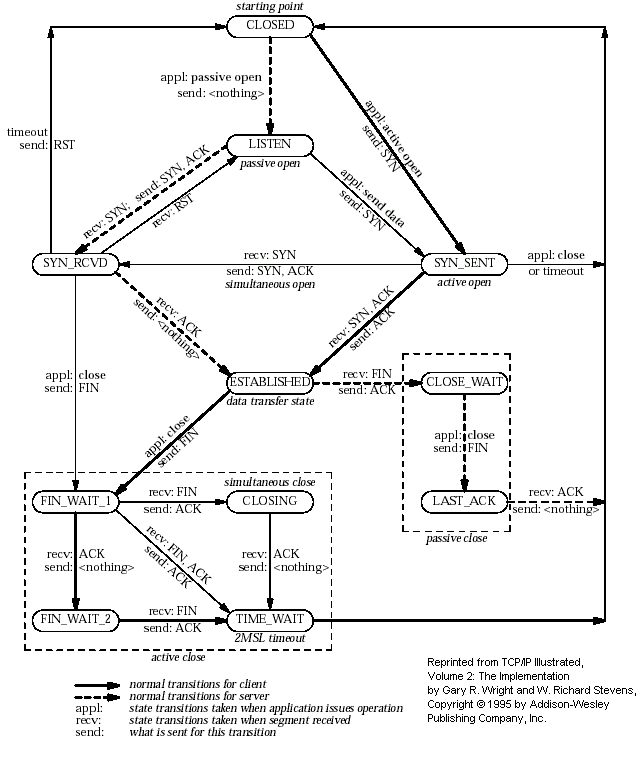
\includegraphics[width=\textwidth]{figures/tcpstate}
\caption{TCP state diagram}
\label{fig:tcp_states}
\end{figure}

\subsection{Flow control}
\label{subsec:flow_control}

The TCP module of the receiver buffers the data of incoming segments.
This buffer has a limited capacity, so it is desirable to notify the sender
about how much data the client can accept. The sender stops the transmission
if this space exhausted.

In TCP every ACK segment holds a Window field; this is the available space
in the receiver buffer. When the sender reads the Window, it can send at most
Window unacknowledged bytes.

\subsubsection*{Window Scale option}

% RFC1323
The TCP segment contains a 16-bit field for the Window, thus allowing at most
65535 byte windows. If the network bandwidth and latency is large, it is surely
too small. The sender should be able to send bandwitdh*latency bytes without
receiving ACKs.

For this purpose the Window Scale (WS) option had been introduced in RFC1323.
This option specifies a scale factor used to interpret the value of the Window field.
The format is the option is:

\begin{center}
\begin{bytefield}{24}
\bitbox{8}{Kind=3} &
\bitbox{8}{Length=3} &
\bitbox{8}{shift.cnt}
\end{bytefield}
\end{center}

If the TCP want to enable window sizes greater than 65535, it should send
a WS option in the SYN segment or SYN/ACK segment (if received a SYN with WS
option). Both sides must send the option in the SYN segment to enable window scaling,
but the scale in one direction might differ from the scale in the other direction.
The $shift.cnt$ field is the 2-base logarithm of the window scale of the sender.
Valid values of $shift.cnt$ are in the $[0,14]$ range.

\subsubsection*{Persistence timer}

When the reciever buffer is full, it sends a 0 length window in the ACK segment
to stop the sender. Later if the application reads the data,
it will repeat the last ACK with an updated window to resume data sending.
If this ACK segment is lost, then the sender is not notified, so a deadlock
happens.

To avoid this situation the sender starts a Persistence Timer when it received
a 0 size window. If the timer expires before the window is increased it send
a probe segment with 1 byte of data. It will receive the current window of the
receiver in the response to this segment.

\subsubsection*{Keepalive timer}

TCP keepalive timer is used to detect dead connections.

\subsection{Transmission policies}
\label{subsec:trans_policies}

\subsubsection*{Retransmissions}

% source: RFC1222 4.3.2.1 and Tannenbaum 6.5.10

When the sender TCP sends a TCP segment it starts a
retransmission timer.
If the ACK arrives before the timer expires it is stopped,
otherwise it triggers a retransmission of the segment.

If the retransmission timeout (RTO) is too high, then lost segments
causes high delays, if it is too low, then the receiver gets
too many useless duplicated segments. For optimal behaviour, the
timeout must be dynamically determined.

Jacobson suggested to measure the RTT mean and deviation
and apply the timeout:

$$ RTO = RTT + 4 * D $$

Here RTT and D are the measured smoothed roundtrip time and its
smoothed mean deviation. They are initialized to 0 and updated each time an
ACK segment received according to the following formulas:

$$ RTT = \alpha*RTT + (1-\alpha) * M $$

$$ D = \alpha*D + (1-\alpha)*|RTT-M| $$

where $M$ is the time between the segments send and the acknowledgment
arrival. Here the $\alpha$ smoothing factor is typically $7/8$.

One problem may occur when computing the round trip: if the
retransmission timer timed out and the segment is sent again,
then it is unclear that the received ACK is a response to the
first transmission or to the second one. To avoid confusing the
RTT calculation, the segments that have been retransmitted
do not update the RTT. This is known as Karn's modification.
He also suggested to double the $RTO$ on each failure until the
segments gets through (``exponential backoff'').

\subsubsection*{Delayed ACK algorithm}

% RFC1122 4.2.3.2

A host that is receiving a stream of TCP data segments can
increase efficiency in both the Internet and the hosts by
sending fewer than one ACK (acknowledgment) segment per data
segment received; this is known as a "delayed ACK" [TCP:5].

Delay is max. 500ms.

A delayed ACK gives the application an opportunity to
update the window and perhaps to send an immediate
response.  In particular, in the case of character-mode
remote login, a delayed ACK can reduce the number of
segments sent by the server by a factor of 3 (ACK,
window update, and echo character all combined in one
segment).

In addition, on some large multi-user hosts, a delayed
ACK can substantially reduce protocol processing
overhead by reducing the total number of packets to be
processed [TCP:5].  However, excessive delays on ACK's
can disturb the round-trip timing and packet "clocking"
algorithms [TCP:7].

% RFC2581 3.2

a TCP receiver SHOULD send an immediate ACK
when the incoming segment fills in all or part of a gap in the
sequence space.

\subsubsection*{Nagle's algorithm}

RFC896 describes the ``small packet problem": when the application
sends single-byte messages to the TCP, and it transmitted immediatly
in a 41 byte TCP/IP packet (20 bytes IP header, 20 bytes TCP header,
1 byte payload), the result is a 4000\% overhead that can cause
congestion in the network.

The solution to this problem is to delay the transmission until
enough data received from the application and send all collected
data in one packet. Nagle proposed that
when a TCP connection has outstanding data that has not
yet been acknowledged, small segments should not be sent
until the outstanding data is acknowledged.

\subsubsection*{Silly window avoidance}

The Silly Window Syndrome (SWS) is described in RFC813. It occurs when
a TCP receiver advertises a small window and the TCP sender immediately
sends data to fill the window. Let's take the example when the sender
process writes a file into the TCP stream in big chunks, while the
receiver process reads the bytes one by one. The first few bytes
are transmitted as whole segments until the receiver buffer
becomes full. Then the application reads one
byte, and a window size 1 is offered to the sender. The sender sends
a segment with 1 byte payload immediately, the receiver buffer becomes
full, and after reading 1 byte, the offered window is 1 byte again.
Thus almost the whole file is transmitted in very small segments.

In order to avoid SWS, both sender and receiver must try to avoid this
situation. The receiver must not advertise small windows and the sender
must not send small segments when only a small window is advertised.

In RFC813 it is offered that
\begin{enumerate}
  \item the receiver should not advertise windows that is smaller than the maximum
        segment size of the connection
  \item the sender should wait until the window is large enough for a maximum sized
        segment.
\end{enumerate}

\subsubsection*{Timestamp option}

Efficient retransmissions depends on precious RTT measurements.
Packet losses can reduce the precision of these measurements radically.
When a segment lost, the ACKs received in that window can not be used;
thus reducing the sample rate to one RTT data per window. This is
unacceptable if the window is large.

The proposed solution to the problem is to use a separate timestamp
field to connect the request and the response on the sender side.
The timestamp is transmitted as a TCP option. The option contains two
32-bit timestamps:

\begin{center}
\begin{bytefield}{80}
\bitbox{8}{Kind=5} &
\bitbox{8}{Length=10} &
\bitbox{32}{TS Value} &
\bitbox{32}{TS Echo Reply} &
\end{bytefield}
\end{center}

Here the TS Value (TSVal) field is the current value of the timestamp
clock of the TCP sending the option, TS Echo Reply (TSecr) field is
0 or echoes the timestamp value of that was sent by the remote TCP.
The TSscr field is valid only in ACK segments that acknowledges new
data. Both parties should send the TS option in their SYN segment
in order to allow the TS option in data segments.

The timestamp option can also be used for PAWS (protection against wrapped
sequence numbers).


\subsection{Congestion control}

Flow control allows the sender to slow down the transmission when the
receiver can not accept them because of memory limitations. However
there are other situations when a slow down is desirable. If the sender
transmits a lot of data into the network it can overload the processing
capacities of the network nodes, so packets are lost in the network
layer.

For this purpose another window is maintained at the sender side, the
congestion window (CWND). The congestion window is a sender-side limit
on the amount of data the sender can transmit into the network before
receiving ACK. More precisely, the sender can send at most max(CWND, WND)
bytes above SND.UNA, therefore $ SND.NXT < SND.UNA + max(CWND, WND) $ is
guaranteed.

The size of the congestion window is dinamically determined by monitoring
the state of the network.

% RFC2581
%
% Definitions:
% SMSS: sender maximum segment size
% RMSS: receiver maximum segment size (default 536)
% rwnd: most recently advertised receiver window
% IW: initial sender's congestion window
% LW: loss window, size of congestion window after a TCP sender detects loss
% RW: restart window, size of congestion window after a TCP restarts transmission after an idle period
% fligth size: amount of data has been sent but not yet acknowledged
% cwnd: congestion window, sender-size limit on the amount of data the sender
%       can transmit into the network before receiving an ACK
% rwnd: receiver advertised window, receiver-side limit on the amount of outstanding data
% sstresh: whether slow start or congestion avoidance used
%
% IW <= 2*MSS


\subsubsection*{Slow Start and Congestion Avoidance}

There are two algorithm that updates the congestion window, ``Slow Start''
and ``Congestion Avoidance''. They are specified in RFC2581.

\begin{pseudocode}
$cwnd \gets 2*SMSS$
$ssthresh \gets $ upper bound of the window (e.g. $65536$)
whenever ACK received
  if $cwnd < ssthresh$
    $cwnd \gets cwnd + SMSS$
  otherwise
    $cwnd \gets cwnd + SMSS*SMSS/cwnd$
whenever packet loss detected
  $cwnd \gets SMSS$
  $ssthresh \gets max(FlightSize/2, 2*SMSS)$
\end{pseudocode}

Slow Start means that when the connection opened the sender initially
sends the data with a low rate. This means that the initial
window (IW) is at most 2 MSS, but no more than 2 segments. If there was no packet loss,
then the congestion window is increased rapidly, it is doubled in each flight.
When a packet loss is detected, the congestion window is reset to 1 MSS (loss window, LW)
and the ``Slow Start'' is applied again.

\begin{note}
RFC3390 increased the IW to roughly 4K bytes: $min(4*MSS, max(2*MSS, 4380))$.
\end{note}

When the congestion window reaches a certain limit (slow start threshold),
the ``Congestion Avoidance'' algorithm is applied. During ``Congestion Avoidance''
the window is incremented by 1 MSS per round-trip-time (RTT). This is usually
implemented by updating the window according to the $ cwnd += SMSS*SMSS/cwnd $
formula on every non-duplicate ACK.

The Slow Start Threshold is updated when a packet loss is detected.
It is set to $max(FlightSize/2, 2*SMSS)$.

How the sender estimates the flight size? The data sent, but not yet acknowledged.

How the sender detect packet loss? Retransmission timer expired.


\subsubsection*{Fast Retransmit and Fast Recovery}

RFC2581 specifies two additional methods to increase the efficiency
of congestion control: ``Fast Retransmit'' and ``Fast Recovery''.

``Fast Retransmit'' requires that the receiver signal the event,
when an out-of-order segment arrives. It is achieved by sending
an immediate duplicate ACK. The receiver also sends an immediate
ACK when the incoming segment fills in a gap or part of a gap.

When the sender receives the duplicated ACK it knows that some
segment after that sequence number is received out-of-order or
that the network duplicated the ACK. If 3 duplicated ACK received
then it is more likely that a segment was dropped or delayed.
In this case the sender starts to retransmit the segments
immediately.

``Fast Recovery'' means that ``Slow Start'' is not applied
when the loss is detected as 3 duplicate ACKs. The arrival
of the duplicate ACKs indicates that the network is not fully
congested, segments after the lost segment arrived, as well
the ACKs.

% Details?
%
%    1.  When the third duplicate ACK is received, set ssthresh to no more
%        than the value given in equation 3.
%
%    2.  Retransmit the lost segment and set cwnd to ssthresh plus 3*SMSS.
%        This artificially "inflates" the congestion window by the number
%        of segments (three) that have left the network and which the
%        receiver has buffered.
%
%    3.  For each additional duplicate ACK received, increment cwnd by
%        SMSS.  This artificially inflates the congestion window in order
%        to reflect the additional segment that has left the network.
%
%    4.  Transmit a segment, if allowed by the new value of cwnd and the
%        receiver's advertised window.
%
%    5.  When the next ACK arrives that acknowledges new data, set cwnd to
%        ssthresh (the value set in step 1).  This is termed "deflating"
%        the window.
%
%        This ACK should be the acknowledgment elicited by the
%        retransmission from step 1, one RTT after the retransmission
%        (though it may arrive sooner in the presence of significant out-
%        of-order delivery of data segments at the receiver).
%        Additionally, this ACK should acknowledge all the intermediate
%        segments sent between the lost segment and the receipt of the
%        third duplicate ACK, if none of these were lost.

\subsubsection*{Loss Recovery Using Limited Transmit}

If there is not enough data to be send after a lost segment,
then the Fast Retransmit algorithm is not activated, but the
costly retranmission timeout used.

RFC3042 suggests that the sender TCP should send a new data segment
in response to each of the first two duplicate acknowledgement. Transmitting
these segments increases the probability that TCP can recover from a single
lost segment using the fast retransmit algorithm, rather than using a costly
retransmission timeout.

\subsubsection*{Selective Acknowledgments}

% RFC2018

With selective
acknowledgments (SACK), the data receiver can inform the sender about all
segments that have arrived successfully, so the sender need
retransmit only the segments that have actually been lost.

With the help of this information the sender can detect
\begin{itemize}
  \item replication by the network
  \item false retransmit due to reordering
  \item retransmit timeout due to ACK loss
  \item early retransmit timeout
\end{itemize}


In the congestion control algorithms described so far
the sender has only rudimentary information about which
segments arrived at the receiver. On the other hand
the algorithms are implemented completely on the sender side,
they only require that the client sends immediate ACKs on
duplicate segments. Therefore they can work in a heterogenous
environment, e.g. a client with Tahoe TCP can communicate with
a NewReno server. On the other hand SACK must be supported by
both endpoint of the connection to be used.

If a TCP supports SACK it includes the \emph{SACK-Permitted} option
in the SYN/SYN-ACK segment when initiating the connection.
The SACK extension enabled for the connection if the \emph{SACK-Permitted}
option was sent and received by both ends. The option occupies
2 octets in the TCP header:

\begin{center}
\begin{bytefield}{16}
\bitbox{8}{Kind=4} &
\bitbox{8}{Length=2}
\end{bytefield}
\end{center}

If the SACK is enabled then the data receiver adds SACK option
to the ACK segments. The SACK option informs the sender about
non-contiguous blocks of data that have been received and queued.
The meaning of the \emph{Acknowledgement Number} is unchanged,
it is still the cumulative sequence number. Octets received
before the \emph{Acknowledgement Number} are kept by the receiver,
and can be deleted from the sender's buffer. However the receiver
is allowed to drop the segments that was only reported in the SACK
option.

The \emph{SACK} option contains the following fields:

\begin{center}
\begin{bytefield}{32}
\bitbox[]{16}{} &
\bitbox{8}{Kind=5} &
\bitbox{8}{Length} \\
\bitbox{32}{Left Edge of 1st Block} \\
\bitbox{32}{Right Edge of 1st Block} \\
\wordbox[]{1}{$\vdots$ \\[1ex]} \\
\bitbox{32}{Left Edge of nth Block} \\
\bitbox{32}{Right Edge of nth Block}
\end{bytefield}
\end{center}

Each block represents received bytes of data that are
contiguous and isolated with one exception: if a segment
received that was already ACKed (i.e. below $RCV.NXT$),
it is included as the first block of the \emph{SACK} option.
The purpose is to inform the sender about a spurious retransmission.

Each block in the option occupies 8 octets. The TCP header
allows 40 bytes for options, so at most 4 blocks can be
reported in the \emph{SACK} option (or 3 if TS option is also used).
The first block is used for reporting the most recently received
data, the following blocks repeats the most recently reported
SACK blocks. This way each segment is reported at least 3 times,
so the sender receives the information even if some ACK segment is
lost.


\textbf{SACK based loss recovery}

% RFC3517: loss recovery based on SACK

Now lets see how the sender can use the information in the
\emph{SACK} option. First notice that it can give a better
estimation of the amount of data outstanding in the network
(called $pipe$ in RFC3517).
If $highACK$ is the highest ACKed sequence number, and
$highData$ of the highest sequence number transmitted,
then the bytes between $highACK$ and $highData$ can be
in the network. However $ pipe \neq highData - highACK $
if there are lost and retransmitted segments:

$$ pipe = highData - highACK - lostBytes + retransmittedBytes $$

A segment is supposed to be lost if it was not received
but 3 segments recevied that comes after this segment in the sequence
number space.
This condition is detected by the sender by receiving
either 3 discontiguous SACKed blocks, or at least
$3*SMSS$ SACKed bytes above the sequence numbers of the
lost segment.

The transmission of data starts with a \emph{Slow Start} phase.
If the loss is detected by 3 duplicate ACK, the sender
goes into the recovery state: it sets
$cwnd$ and $ssthresh$ to $FlightSize / 2$.
It also remembers the $highData$ variable, because
the recovery state is left when this sequence number
is acknowledged.

In the recovery state it sends data
until there is space in the congestion window (i.e. $cwnd-pipe >= 1 SMSS$)
The data of the segment is choosen by the following rules (first rule that applies):

\begin{enumerate}
  \item send segments that is lost and not yet retransmitted
  \item send segments that is not yet transmitted
  \item send segments that is not yet retransmitted and possibly fills a gap
        (there is SACKed data above it)
\end{enumerate}

If there is no data to send, then the sender waits for the next ACK, updates
its variables based on the data of the received ACK, and then try to transmit
according to the above rules.

If an RTO occurs, the sender drops the collected SACK information and
initiates a Slow Start. This is to avoid a deadlock when the receiver
dropped a previously SACKed segment.

% highACK: highest ACKed sequence number
%
% highData: highest sequence number transmitted
%
% highRxt: highest sequence number which has been retransmitted
%
%
% Normal phase: before the first loss, until 3 duplicate ACK
%
% Loss recovery phase: until ACK for RecoveryPoint received
%
% On the transition to loss recovery phase
% \begin{enumerate}
%   \item RecoveryPoint=HighData
%   \item ssthresh=cwnd=FlightSize/2
%   \item compute \emph{pipe}
% \end{enumerate}
%
% In the loss recovery phase, for each incoming ACK:
%
% \begin{enumerate}
%   %\Alph
%   \item if cumulative ACK above RecoveryPoint, leave loss recovery phase
%   \item update SACK info and compute pipe
%   \item if $cwnd-pipe >= 1 SMSS$ send one or more segments (if there is data to send)
%   \item update HighRxt, HighData according to the sent bytes
%   \item increment $pipe$ by the amount of data sent
%   \item if $cwnd-pipe >= 1 SMSS$, continue sending
% \end{enumerate}
%
% Which bytes to be send are determined as follows:
%
% \begin{enumerate}
%   \item if there is a byte which is lost and not yet retransmitted, send that in 1 segment
%   \item otherwise if there is unsent data, send that in 1 segment
%   \item otherwise if there is not yet retransmitted data, and above that there is SACKed data, send that
%   \item otherwise there is no data to send
% \end{enumerate}


\section{TCP module}

The \nedtype{TCP} simple module is the main implementation of the TCP protocol in the INET framework.
Other implementation are described in section \ref{sec:other_tcp}.
The \nedtype{TCP} module as other transport protocols work above the network layer and below the application
layer, therefore it has gates to be connected with the IPv4 or IPv6 network (ipIn/ipOut or ipv6In/ipv6Out),
and with the applications (appIn[k], appOut[k]).
One \nedtype{TCP} module can serve several application modules, and several
connections per application. The $k$th application connects to \nedtype{TCP}'s
\ttt{appIn[k]} and \ttt{appOut[k]} ports.

The TCP module usually specified by its module interface
(\nedtype{ITCP}) in the NED definition of hosts, so it can be replaced with any implementation
that communicates through the same gates. The \nedtype{TCP} model relies on
sending and receiving \cppclass{IPControlInfo} objects
attached to TCP segment objects as control info (see \ffunc{cMessage::setControlInfo()}).

The \nedtype{TCP} module manages several \cppclass{TCPConnection} object each
holding the state of one connection. The connections are identified
by a connection identifier which is choosen by the application.
If the connection is established it can also be identified by
the local and remote addresses and ports. The TCP module simply
dispatches the incoming application commands and packets to
the corresponding object.

\subsection{TCP packets}
\label{subsec:tcp_packets}

The INET framework models the TCP header with the \msgtype{TCPSegment} message class.
This contains the fields of a TCP frame, except:
\begin{compactitem}
  \item \emph{Data Offset}: represented by \ffunc{cMessage::length()}
  \item \emph{Reserved}
  \item \emph{Checksum}: modelled by \ffunc{cMessage::hasBitError()}
  \item \emph{Options}: only EOL, NOP, MSS, WS, SACK\_PERMITTED, SACK and TS are possible
  \item \emph{Padding}
\end{compactitem}

The Data field can either be represented by (see \cppclass{TCPDataTransferMode}):
\begin{compactitem}
  \item encapsulated C++ packet objects,
  \item raw bytes as a \cppclass{ByteArray} instance,
  \item its byte count only,
\end{compactitem}
corresponding to transfer modes OBJECT, BYTESTREAM, BYTECOUNT resp.


\subsection{TCP commands}

The application and the TCP module communicates with each other
by sending \cppclass{cMessage} objects. These messages are specified
in the \ffilename{TCPCommand.msg} file.

The \cppclass{TCPCommandCode} enumeration defines the message kinds
that are sent by the application to the TCP:
\begin{itemize}
  \item TCP\_C\_OPEN\_ACTIVE: active open
  \item TCP\_C\_OPEN\_PASSIVE: passive open
  \item TCP\_C\_SEND: send data
  \item TCP\_C\_CLOSE: no more data to send
  \item TCP\_C\_ABORT: abort connection
  \item TCP\_C\_STATUS: request status info from TCP
\end{itemize}

Each command message should have an attached control info of type \cppclass{TCPCommand}.
Some commands (TCP\_C\_OPEN\_xxx, TCP\_C\_SEND) use subclasses.
The \cppclass{TCPCommand} object has a \fvar{connId} field that identifies the
connection locally within the application. \fvar{connId} is to be chosen by the
application in the open command.

When the application receives a message from the TCP, the message kind is
set to one of the \cppclass{TCPStatusInd} values:
\begin{itemize}
  \item TCP\_I\_ESTABLISHED: connection established
  \item TCP\_I\_CONNECTION\_REFUSED: connection refused
  \item TCP\_I\_CONNECTION\_RESET: connection reset
  \item TCP\_I\_TIME\_OUT: connection establish timer went off, or max retransmission count reached
  \item TCP\_I\_DATA: data packet
  \item TCP\_I\_URGENT\_DATA: urgent data packet
  \item TCP\_I\_PEER\_CLOSED: FIN received from remote TCP
  \item TCP\_I\_CLOSED: connection closed normally
  \item TCP\_I\_STATUS: status info
\end{itemize}

These messages also have an attached control info with \cppclass{TCPCommand}
or derived type (TCPConnectInfo, TCPStatusInfo, TCPErrorInfo).

% receive() calls are not modeled, incoming data passed to the application right away
% how accurate the modeling of the receiver window?

\subsection{TCP parameters}

The \nedtype{TCP} module has the following parameters:
\begin{itemize}
  \item \fpar{advertisedWindow} in bytes, corresponds with the maximal receiver buffer capacity (Note: normally, NIC queues should be at least this size, default is  14*mss)
  \item \fpar{delayedAcksEnabled} delayed ACK algorithm (RFC 1122) enabled/disabled
  \item \fpar{nagleEnabled} Nagle's algorithm (RFC 896) enabled/disabled
  \item \fpar{limitedTransmitEnabled} Limited Transmit algorithm (RFC 3042) enabled/disabled (can be used for TCPReno/TCPTahoe/TCPNewReno/TCPNoCongestionControl)
  \item \fpar{increasedIWEnabled} Increased Initial Window (RFC 3390) enabled/disabled
  \item \fpar{sackSupport} Selective Acknowledgment (RFC 2018, 2883, 3517) support (header option) (SACK will be enabled for a connection if both endpoints support it)
  \item \fpar{windowScalingSupport} Window Scale (RFC 1323) support (header option) (WS will be enabled for a connection if both endpoints support it)
  \item \fpar{timestampSupport} Timestamps (RFC 1323) support (header option) (TS will be enabled for a connection if both endpoints support it)
  \item \fpar{mss} Maximum Segment Size (RFC 793) (header option, default is 536)
  \item \fpar{tcpAlgorithmClass} the name of TCP flavour

             Possible values are ``TCPReno'' (default), ``TCPNewReno'', ``TCPTahoe'', ``TCPNoCongestionControl'' and ``DumpTCP''.
             In the future, other classes can be written which implement Vegas, LinuxTCP  or other variants.
             See section \ref{sec:tcp_algorithms} for detailed description of implemented flavours.

             Note that TCPOpenCommand allows tcpAlgorithmClass to be chosen per-connection.

  \item \fpar{recordStats} if set to false it disables writing excessive amount of output vectors
\end{itemize}

\subsection{Statistics}

The \nedtype{TCP} module collects the following vectors:

\begin{tabular}{l p{10cm}}
  \ttt{send window} & $SND.WND$ \\
  \ttt{receive window} & $RCV.WND$, after SWS avoidance applied \\
  \ttt{advertised window} & $RCV.NXT + RCV.WND$ \\
  \ttt{sent seq} & \emph{Sequence Number} of the sent segment \\
  \ttt{sent ack} & \emph{Acknowledgement Number} of the sent segment \\
  \ttt{rcvd seq} & \emph{Sequence Number} of the received segment \\
  \ttt{rcvd ack} & \emph{Acknowledgement Number} of the received segment \\
  \ttt{unacked bytes} & number of sent and unacknowledged bytes ($max of SND.NXT - SND.UNA$) \\
  \ttt{rcvd dupAcks} & number of duplicate acknowledgements, reset to 0 when $SND.UNA$ advances \\
  \ttt{pipe} & the value of the SACK $pipe$ variable
               (estimated number of bytes outstanding in the network) \\
  \ttt{sent sacks} & number of SACK blocks sent \\
  \ttt{rcvd sacks} & number of SACK blocks received \\
  \ttt{rcvd oooseg} & number of received out-of-order segments \\
  \ttt{rcvd naseg} & number of received unacceptable segments (outside the receive window) \\
  \ttt{rcvd sackedBytes} & total amount of SACKed bytes in the buffer of the sender \\
  \ttt{tcpRcvQueueBytes} & number of bytes in the receiver's buffer \\
  \ttt{tcpRcvQueueDrops} & number of bytes dropped by the receiver (not enough buffer) \\
  \ttt{cwnd} & congestion window \\
  \ttt{ssthresh} & slow start threshold \\
  \ttt{measured RTT} & measured round trip time \\
  \ttt{smoothed RTT} & smoothed round trip time \\
  \ttt{RTTVAR} & measured smoothed variance of round trip time \\
  \ttt{RTO} & retransmission timeout \\
  \ttt{numRTOs} & number of retransmission timeouts occured \\
\end{tabular}

If the \fpar{recordStats} parameter is set to \fkeyword{false}, then none
of these output vectors are generated.

% \subsection{Animation effects}
%
% TCP module text: number of connections sorted by state
%
% log, log verbose

\section{TCP connections}

Most part of the TCP specification is implemented in the
\cppclass{TCPConnection} class: takes care of the state machine,
stores the state variables (TCB), sends/receives SYN, FIN, RST, ACKs, etc.
TCPConnection itself implements the basic TCP ``machinery'',
the details of congestion control are factored out to
\cppclass{TCPAlgorithm} classes.

There are two additional objects the \cppclass{TCPConnection}
relies on internally: instances of \cppclass{TCPSendQueue} and
\cppclass{TCPReceiveQueue}. These polymorph classes manage the actual data stream,
so \cppclass{TCPConnection} itself only works with sequence number variables.
This makes it possible to easily accomodate need for various types of
simulated data transfer: real byte stream, "virtual" bytes (byte counts
only), and sequence of \cppclass{cMessage} objects (where every message object is
mapped to a TCP sequence number range).

\subsection{Data transfer modes}

Different applications have different needs how to represent
the messages they communicate with. Sometimes it is enough to
simulate the amount of data transmitted (``200 MB''), contents
does not matter. In other scenarios contents matters a lot.
The messages can be represented as a stream of bytes, but
sometimes it is easier for the applications to pass message
objects to each other (e.g. HTTP request represented by a
\msgtype{HTTPRequest} message class).

The TCP modules in the INET framework support 3 data transfer modes:

\begin{itemize}
  \item \ttt{TCP\_TRANSFER\_BYTECOUNT}: only byte counts are
        represented, no actual payload in \msgtype{TCPSegment}s.
        The TCP sends as many TCP segments as needed
  \item \ttt{TCP\_TRANSFER\_BYTESTREAM}: the application can pass
        byte arrays to the TCP. The sending TCP breaks down the bytes
        into MSS sized chunks and transmits them as the payload
        of the TCP segments. The receiving application can read the
        chunks of the data.
  \item \ttt{TCP\_TRANSFER\_OBJECT}: the application pass a
        \cppclass{cMessage} object to the TCP. The sending
        TCP sends as many TCP segments as needed according to
        the message length. The \cppclass{cMessage} object
        is also passed as the payload of the first segment. % check: first?
        The receiving application receives the object only
        when its last byte is received.
\end{itemize}

These values are defined in \ffilename{TCPCommand.msg} as
the \cppclass{TCPDataTransferMode} enumeration. The application
can set the data transfer mode per connection when the connection
is opened. The client and the server application must specify
the same data transfer mode.


\subsection{Opening connections}

Applications can open a local port for incoming connections by sending
the TCP a TCP\_C\_PASSIVE\_OPEN message. The attached control info
(an \cppclass{TCPOpenCommand}) contains the local address and port.
The application can specify that it wants to handle
only one connection at a time, or multiple simultanous connections. If the
\fvar{fork} field is true, it emulates the Unix accept(2) semantics: a new
connection structure is created for the connection (with a new \fvar{connId}),
and the connection with the old connection id remains listening.
If \fvar{fork} is false, then the first connection is accepted
(with the original \fvar{connId}),
and further incoming connections will be refused by the TCP by sending an RST segment.
The \fvar{dataTransferMode} field in \cppclass{TCPOpenCommand} specifies
whether the application data is transmitted as C++ objects, real bytes or byte
counts only. The congestion control algorithm can also be specified
on a per connection basis by setting \fvar{tcpAlgorithmClass} field to the
name of the algorithm.

The application opens a connection to a remote server by sending the TCP
a TCP\_C\_OPEN\_ACTIVE command. The TCP creates a \cppclass{TCPConnection}
object an sends a SYN segment. The initial sequence number selected according
to the simulation time: 0 at time 0, and increased by 1 in each 4$\mu$s.
If there is no response to the SYN segment, it retry after 3s, 9s, 21s and
45s. After 75s a connection establishment timeout (TCP\_I\_TIMEOUT) reported
to the application and the connection is closed.

When the connection gets established, TCP sends a TCP\_I\_ESTABLISHED
notification to the application. The attached control info
(a \cppclass{TCPConnectInfo} instance)
will contain the local and remote addresses and ports of the connection.
If the connection is refused by the remote peer (e.g. the port is not open),
then the application receives a TCP\_I\_CONNECTION\_REFUSED message.

\begin{note}
If you do active OPEN, then send data and close before the connection
has reached ESTABLISHED, the connection will go from SYN\_SENT to CLOSED
without actually sending the buffered data. This is consistent with
RFC 793 but may not be what you would expect.
\end{note}

\begin{note}
Handling segments with SYN+FIN bits set (esp. with data too) is
inconsistent across TCPs, so check this one if it is of importance.
\end{note}

\subsection{Sending Data}

The application can write data into the connection
by sending a message with TCP\_C\_SEND kind to the TCP.
The attached control info must be of type \cppclass{TCPSendCommand}.

The TCP will add the message to the \emph{send queue}.
There are three type of send queues corresponding to the
three data transfer mode. If the payload is transmitted as a message
object, then \cppclass{TCPMsgBasedSendQueue};
if the payload is a byte array then \cppclass{TCPDataStreamSendQueue};
if only the message lengths are represented then \cppclass{TCPVirtualDataSendQueue}
are the classes of send queues. The appropriate queue is created based
on the value of the \fpar{dataTransferMode} parameter of the Open command, no
further configuration is needed.

The message is handed over to the IP when there is
enough room in the windows. If Nagle's algorithm is
enabled, the TCP will collect 1 SMSS data and sends
them toghether.

\begin{note}
There is no way to set the PUSH and URGENT flags, when sending data.
\end{note}

% FIXME urgBit is never set
% FIXME model TCP_NODELAY, there is no PUSH flag in socket.send() (TCP_PUSH option ?)

\subsection{Receiving Data}

The TCP connection stores the incoming segments in the
\emph{receive queue}. The receive queue also has three flavours:
\cppclass{TCPMsgBasedRcvQueue}, \cppclass{TCPDataStreamRcvQueue}
and \cppclass{TCPVirtualDataRcvQueue}. The queue is created
when the connection is opened according to the \fvar{dataTransferMode}
of the connection.

Finite receive buffer size is modeled by the \fpar{advertisedWindow}
parameter. If receive buffer is exhausted (by out-of-order
segments) and the payload length of a new received segment
is higher than the free receiver buffer, the new segment will be dropped.
Such drops are recorded in \emph{tcpRcvQueueDrops} vector.

If the \emph{Sequence Number} of the received segment is the next
expected one, then the data is passed
to the application immediately. The \ffunc{recv()} call of
Unix is not modeled.

The data of the segment, which can be either a \cppclass{cMessage}
object, a \cppclass{ByteArray} object, or a simply byte count,
is passed to the application in a message that has
TCP\_I\_DATA kind.

% when the cMessage object is passed to the app? when last byte received?

\begin{note}
The TCP module does not handle the segments with PUSH or URGENT
flags specially. The data of the segment passed to the application
as soon as possible, but the application can not find out if that
data is urgent or pushed.
\end{note}

\subsection{RESET handling}

When an error occures at the TCP level, an RST segment is sent to
the communication partner and the connection is aborted.
Such error can be:
\begin{compactitem}
  \item arrival of a segment in CLOSED state
  \item an incoming segment acknowledges something not yet sent.
\end{compactitem}

The receiver of the RST it will abort the connection.
If the connection is not yet established, then the passive
end will go back to the LISTEN state and waits for another
incoming connection instead of aborting.

\subsection{Closing connections}

When the application does not have more data to send, it closes the
connection by sending a TCP\_C\_CLOSE command to the TCP. The TCP
will transmit all data from its buffer and in the last segment sets
the FIN flag. If the FIN is not acknowledged in time it will be
retransmitted with exponential backoff.

The TCP receiving a FIN segment will notify the application that
there is no more data from the communication partner. It sends
a TCP\_I\_PEER\_CLOSED message to the application containing
the connection identifier in the control info.

When both parties have closed the connection, the applications
receive a TCP\_I\_CLOSED message and the connection object is
deleted. (Actually one of the TCPs waits for $2 MSL$ before
deleting the connection, so it is not possible to reconnect
with the same addresses and port numbers immediately.)

\subsection{Aborting connections}

The application can also abort the connection. This means that
it does not wait for incoming data, but drops the data associated
with the connection immediately. For this purpose the application
sends a TCP\_C\_ABORT message specifying the connection identifier
in the attached control info. The TCP will send a RST to the
communication partner and deletes the connection object. The application
should not reconnect with the same local and remote addresses and
ports within MSL (maximum segment lifetime), because segments
from the old connection might be accepted in the new one.

\subsection{Status Requests}

Applications can get detailed status information about an existing
connection. For this purpose they send the TCP module a TCP\_C\_STATUS
message attaching an \cppclass{TCPCommand} info with the identifier
of the connection. The TCP will respond with a TCP\_I\_STATUS message
with a \cppclass{TCPStatusInfo} attachement. This control info
contains the current state, local and remote addresses and ports,
the initial sequence numbers, windows of the receiver and sender, etc.

% \section{TCP queues}
%
% Three queues belong to each TCP connection. The \emph{send queue} holds
% the segments not yet transmitted or not yet acknowledged.
% The \emph{receive queue} holds the segments received by the TCP,
% but not yet passed to the application. (This happens only when the segment
% is received out-of-order.). The \emph{retransmit queue} holds additional
% information about the segments in the send queue.
%
% As mentioned in section \ref{subsec:tcp_packets}, there are three methods
% to represent the application data in the TCP segment. Consequently the above
% queues comes in three flavours. If the payload is transmitted as a message
% object, then \cppclass{TCPMsgBasedRcvQueue} and \cppclass{TCPMsgBasedSendQueue};
% if the payload is a byte array then \cppclass{TCPDataStreamRcvQueue} and
% \cppclass{TCPDataStreamSendQueue}; if only the message lengths are represented
% then \cppclass{TCPVirtualDataRcvQueue} and \cppclass{TCPVirtualDataSendQueue}
% are the classes of receive/send queues. The appropriate queue is created based
% on the value of the \fpar{dataTransferMode} parameter of the Open command, no
% further configuration is needed. The retransmit queue is always an
% instance of \cppclass{TCPSACKRexmitQueue}.
%
% The interfaces of the receive/send queues are defined by the
% \cppclass{TCPReceiveQueue} and \cppclass{TCPSendQueue} classes.
%
% % mapping segments into the sequence space
%

\section{TCP algorithms}
\label{sec:tcp_algorithms}

The \cppclass{TCPAlgorithm} object controls
retransmissions, congestion control and ACK sending: delayed acks, slow start,
fast retransmit, etc. They are all extends the \cppclass{TCPAlgorithm} class.
This simplifies the design of \cppclass{TCPConnection} and makes it a lot easier to
implement TCP variations such as Tahoe, NewReno, Vegas or LinuxTCP.

Currently implemented algorithm classes are \cppclass{TCPReno},
\cppclass{TCPTahoe}, \cppclass{TCPNewReno}, \cppclass{TCPNoCongestionControl}
and \cppclass{DumbTCP}. It is also possible to add new TCP variations
by implementing \cppclass{TCPAlgorithm}.

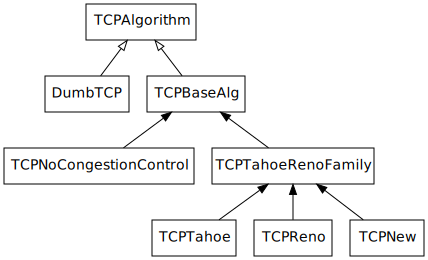
\includegraphics{figures/tcp_algorithms}

The concrete TCP algorithm class to use can be chosen per connection (in OPEN)
or in a module parameter.

\subsection{DumbTCP}

A very-very basic \cppclass{TCPAlgorithm} implementation, with hardcoded
retransmission timeout (2 seconds) and no other sophistication. It can be
used to demonstrate what happened if there was no adaptive
timeout calculation, delayed acks, silly window avoidance,
congestion control, etc. Because this algorithm does not
send duplicate ACKs when receives out-of-order segments,
it does not work well together with other algorithms.

\subsection{TCPBaseAlg}

The \cppclass{TCPBaseAlg} is the base class of the INET implementation
of Tahoe, Reno and New Reno. It implements basic TCP
algorithms for adaptive retransmissions, persistence timers,
delayed ACKs, Nagle's algorithm, Increased Initial Window
-- EXCLUDING congestion control. Congestion control
is implemented in subclasses.

\subsubsection*{Delayed ACK}

When the \fpar{delayedAcksEnabled} parameter is set to \fkeyword{true},
\cppclass{TCPBaseAlg} applies a 200ms delay before sending ACKs.

\subsubsection*{Nagle's algorithm}

When the \fpar{nagleEnabled} parameter is \fkeyword{true}, then
the algorithm does not send small segments if there is outstanding
data. See also \ref{subsec:trans_policies}.

\subsubsection*{Persistence Timer}

The algorithm implements \emph{Persistence Timer} (see \ref{subsec:flow_control}).
When a zero-sized window is received it starts the timer with 5s timeout.
If the timer expires before the window is increased, a 1-byte probe is
sent. Further probes are sent after 5, 6, 12, 24, 48, 60, 60, 60, ...
seconds until the window becomes positive.

\subsubsection*{Initial Congestion Window}

Congestion window is set to 1 SMSS when the connection is established.
If the \fpar{increasedIWEnabled} parameter is true, then the initial
window is increased to 4380 bytes, but at least 2 SMSS and at most 4 SMSS.
The congestion window is not updated afterwards; subclasses can
add congestion control by redefining virtual methods of the
\cppclass{TCPBaseAlg} class.

\subsubsection*{Duplicate ACKs}

The algorithm sends a duplicate ACK when an out-of-order
segment is received or when the incoming segment fills in all
or part of a gap in the sequence space.

\subsubsection*{RTO calculation}

Retransmission timeout ($RTO$) is calculated according to
Jacobson algorithm (with $\alpha=7/8$), and Karn's modification is also applied.
The initial value of the $RTO$ is 3s, its minimum is 1s,
maximum is 240s (2 MSL).

% FIXME according to RFC1222, MIN_REXMIT_TIMEOUT should be a fraction of second
%       to accomodate high speed LANs. In the linux kernel (net/tcp.h)
%       TCP_RTO_MIN is HZ/5 = 200ms. Consider 0ms lower bound.

\subsection{TCPNoCongestion}

TCP with no congestion control (i.e. congestion window kept very large).
Can be used to demonstrate effect of lack of congestion control.

% FIXME 65536 is not 'very large' nowadays, with window scaling
%       the receive window can be as large as 2^30 bytes.
%       Consequently the initial ssthresh is too small for Tahoe/Reno/NewReno,
%       Slow Start is stopped too early first time.

\subsection{TCPTahoe}

The \cppclass{TCPTahoe} algorithm class extends \cppclass{TCPBaseAlg}
with \emph{Slow Start}, \emph{Congestion Avoidance} and
\emph{Fast Retransmit} congestion control algorithms.
This algorithm initiates a \emph{Slow Start} when a packet
loss is detected.

\subsubsection*{Slow Start}

The congestion window is initially set to 1 SMSS or in case of
\fpar{increasedIWEnabled} is \fkeyword{true} to 4380 bytes
(but no less than 2 SMSS and no more than 4 SMSS). The window
is increased on each incoming ACK by 1 SMSS, so it is approximately
doubled in each RTT.

\subsubsection*{Congestion Avoidance}

When the congestion window exceeded $ssthresh$, the window
is increased by $SMSS^2/cwnd$ on each incoming ACK event, so
it is approximately increased by 1 SMSS per RTT.

\subsubsection*{Fast Retransmit}

When the 3rd duplicate ACK received, a packet loss is detected
and the packet is retransmitted immediately. Simultanously
the $ssthresh$ variable is set to half of the $cwnd$ (but at least 2 SMSS)
and $cwnd$ is set to 1 SMSS, so it enters slow start again.

Retransmission timeouts are handled the same way:
$ssthresh$ will be $cwnd/2$, $cwnd$ will be 1 SMSS.

\subsection{TCPReno}

The \cppclass{TCPReno} algorithm extends the behaviour \cppclass{TCPTahoe}
with \emph{Fast Recovery}. This algorithm can also use the information
transmitted in SACK options, which enables a much more accurate
congestion control.

\subsubsection*{Fast Recovery}

When a packet loss is detected by receiveing 3 duplicate ACKs,
$ssthresh$ set to half of the current window as in Tahoe. However
$cwnd$ is set to $ssthresh + 3*SMSS$ so it remains in congestion
avoidance mode. Then it will send one new segment for each incoming
duplicate ACK trying to keep the pipe full of data. This requires
the congestion window to be inflated on each incoming duplicate
ACK; it will be deflated to $ssthresh$ when new data gets
acknowledged.

However a hard packet loss (i.e. RTO events) cause a
slow start by setting $cwnd$ to 1 SMSS.

\subsubsection*{SACK congestion control}

This algorithm can be used with the SACK extension.
Set the \fpar{sackSupport} parameter to \fkeyword{true} to
enable sending and receiving \emph{SACK} options.

\subsection{TCPNewReno}

This class implements the TCP variant known as New Reno.
New Reno recovers more efficiently from multiple packet losses within one RTT
than Reno does.

It does not exit fast-recovery phase until all data which was out-standing
at the time it entered fast-recovery is acknowledged. Thus avoids
reducing the $cwnd$ multiple times.

\section{TCP socket}

%The \cppclass{TCPSocket} C++ class is provided to simplify managing TCP connections
%from applications. \cppclass{TCPSocket} handles the job of assembling and sending
%command messages (OPEN, CLOSE, etc) to \nedtype{TCP}, and it also simplifies
%the task of dealing with packets and notification messages coming from \nedtype{TCP}.

\cppclass{TCPSocket} is a convenience class, to make it easier to manage TCP connections
from your application models. You'd have one (or more) \cppclass{TCPSocket} object(s)
in your application simple module class, and call its member functions
(bind(), listen(), connect(), etc.) to open, close or abort a TCP connection.

TCPSocket chooses and remembers the connId for you, assembles and sends command
packets (such as OPEN\_ACTIVE, OPEN\_PASSIVE, CLOSE, ABORT, etc.) to TCP,
and can also help you deal with packets and notification messages arriving
from TCP.

A session which opens a connection from local port 1000 to 10.0.0.2:2000,
sends 16K of data and closes the connection may be as simple as this
(the code can be placed in your \ffunc{handleMessage()} or
\ffunc{activity()}):

\begin{cpp}
TCPSocket socket;
socket.connect(IPvXAddress("10.0.0.2"), 2000);

msg = new cMessage("data1");
msg->setByteLength(16*1024);  16K
socket.send(msg);

socket.close();
\end{cpp}

% FIXME missing setOutputGate() call

Dealing with packets and notification messages coming from TCP is somewhat
more cumbersome. Basically you have two choices: you either process those
messages yourself, or let TCPSocket do part of the job. For the latter,
you give TCPSocket a callback object on which it'll invoke the appropriate
member functions: \ffunc{socketEstablished()}, \ffunc{socketDataArrived()},
\ffunc{socketFailure()}, \ffunc{socketPeerClosed()},
etc (these are methods of \cppclass{TCPSocket::CallbackInterface}).,
The callback object can be your simple module class too.

This code skeleton example shows how to set up a TCPSocket to use the module
itself as callback object:

\begin{cpp}
class MyModule : public cSimpleModule, public TCPSocket::CallbackInterface
{
    TCPSocket socket;
    virtual void socketDataArrived(int connId, void *yourPtr,
                                   cPacket *msg, bool urgent);
    virtual void socketFailure(int connId, void *yourPtr, int code);
    ...
};

void MyModule::initialize() {
    socket.setCallbackObject(this,NULL);
}

void MyModule::handleMessage(cMessage *msg) {
    if (socket.belongsToSocket(msg))
        socket.processMessage(msg); dispatch to socketXXXX() methods
    else
        ...
}

void MyModule::socketDataArrived(int, void *, cPacket *msg, bool) {
    ev << "Received TCP data, " << msg->getByteLength() << " bytes\\n";
    delete msg;
}

void MyModule::socketFailure(int, void *, int code) {
    if (code==TCP_I_CONNECTION_RESET)
        ev << "Connection reset!\\n";
    else if (code==TCP_I_CONNECTION_REFUSED)
        ev << "Connection refused!\\n";
    else if (code==TCP_I_TIMEOUT)
        ev << "Connection timed out!\\n";
}
\end{cpp}

If you need to manage a large number of sockets (e.g. in a server
application which handles multiple incoming connections), the
\cppclass{TCPSocketMap} class may be useful. The following code
fragment to handle incoming connections is from the LDP module:

\begin{cpp}
TCPSocket *socket = socketMap.findSocketFor(msg);
if (!socket)
{
    not yet in socketMap, must be new incoming connection: add to socketMap
    socket = new TCPSocket(msg);
    socket->setOutputGate(gate("tcpOut"));
    socket->setCallbackObject(this, NULL);
    socketMap.addSocket(socket);
}
dispatch to socketEstablished(), socketDataArrived(), socketPeerClosed()
or socketFailure()
socket->processMessage(msg);
\end{cpp}

\section{Other TCP implementations}
\label{sec:other_tcp}

INET contains two other implementation of the TCP protocol:
\nedtype{TCP\_lwIP} and \nedtype{TCP\_NSC}.
All TCP modules implements the \nedtype{ITCP} interface and
communicate with the application and the IP layer through the
same interface. Therefore they can be interchanged and can
operate with each other. See \ffilename{examples/inet/tcpclientserver/omnetpp.ini}
how to parametrize \nedtype{StandardHost}s to use the different
implementations.

\subsection{TCP LWIP}

lwIP is a light-weight implementation of the TCP/IP protocol suite
that was originally written by Adam Dunkels of the Swedish Institute of
Computer Science. The current development homepage is
\url{http://savannah.nongnu.org/projects/lwip/}.

The implementation targets embedded devices: it has
very limited resource usage (it works ``with tens of kilobytes of RAM and
around 40 kilobytes of ROM'') and does not require an underlying OS.

The \nedtype{TCP\_lwIP} simple module is based on the 1.3.2 version of
the lwIP sources.

Features:

\begin{compactitem}
\item delayed ACK
\item Nagle's algorithm
\item round trip time estimation
\item adaptive retransmission timeout
\item SWS avoidance
\item slow start threshold
\item fast retransmit
\item fast recovery
\item persist timer
\item keep-alive timer
\end{compactitem}

\subsubsection*{Limitations}

\begin{itemize}
  \item only MSS and TS TCP options are supported. The TS option is turned off
        by default, but can be enabled by defining LWIP\_TCP\_TIMESTAMPS to 1
        in \ffilename{lwipopts.h}.
  \item \fvar{fork} must be \fkeyword{true} in the passive open command
  \item The status request command (TCP\_C\_STATUS) only reports the
          local and remote addresses/ports of the connection and
          the MSS, SND.NXT, SND.WND, SND.WL1, SND.WL2, RCV.NXT, RCV.WND variables.
\end{itemize}

% lwIP license file missing from INET source
% FIXME TCP_lwIP uses only connId to identify the connection instead of (connId,appGateIndex)
% FIXME status command returns message kind TCP_C_STATUS instead of TCP_I_STATUS

\subsubsection*{Statistics}

The \nedtype{TCP\_lwIP} module generates the following vector files:

\begin{itemize}
  \item \ttt{send window}: value of the $SND.WND$ variable
  \item \ttt{sent seq}: \emph{Sequence Number} of the sent segment
  \item \ttt{sent ack}: \emph{Acknowledgment Number } of the sent segment
  \item \ttt{receive window}: value of the $RCV.WND$ variable
  \item \ttt{rcvd seq}: \emph{Sequence Number} of the received segment
  \item \ttt{rcvd acq}: \emph{Acknowledgment Number} of the received segment
\end{itemize}

% FIXME the following vectors are created, but not used (copy paste?):
%       'sent sacks', 'advertised window', 'rcvd sacks', 'unacked bytes',
%       'rcvd dupAcks', 'pipe', 'rcvd oooseg', 'rcvd sackedBytes',
%       'tcpRcvQueueBytes', 'tcpRcvQueueDrops'
The creation of these vectors can be disabled by setting the \fpar{recordStats}
parameter to \fkeyword{false}.


\subsection{TCP NSC}

Network Simulation Cradle (NSC) is a tool that allow real-world TCP/IP network stacks
to be used in simulated networks. The NSC project is created by Sam Jansen
and available on \url{http://research.wand.net.nz/software/nsc.php}. NSC currently
contains Linux, FreeBSD, OpenBSD and lwIP network stacks, altough on 64-bit
systems only Linux implementations can be built.

To use the \nedtype{TCP\_NSC} module you should download the
\ffilename{nsc-0.5.2.tar.bz2} package and follow the instructions
in the \ffilename{<inet\_root>/3rdparty/README} file to build it.

\begin{warning}
Before generating the INET module, check that the \emph{opp\_makemake} call
in the make file (\ffilename{<inet\_root>/Makefile}) includes the
\emph{-DWITH\_TCP\_NSC} argument. Without this option the \nedtype{TCP\_NSC}
module is not built. If you build the INET library from the IDE, it is enough
to enable the \emph{TCP (NSC)} project feature.
\end{warning}

\subsubsection*{Parameters}

The \nedtype{TCP\_NSC} module has the following parameters:

\begin{itemize}
  \item \fpar{stackName}: the name of the TCP implementation to be used.
  Possible values are: \ttt{liblinux2.6.10.so}, \ttt{liblinux2.6.18.so},
  \ttt{liblinux2.6.26.so}, \ttt{libopenbsd3.5.so}, \ttt{libfreebsd5.3.so} and
  \ttt{liblwip.so}. (On the 64 bit systems, the \ttt{liblinux2.6.26.so} and
  \ttt{liblinux2.6.16.so} are available only).

  \item \fpar{stackBufferSize}: the size of the receive and send buffer of
  one connection for selected TCP implementation.
  The NSC sets the \fvar{wmem\_max}, \fvar{rmem\_max}, \fvar{tcp\_rmem}, \fvar{tcp\_wmem}
  parameters to this value on linux TCP implementations. For details, you can see
  the NSC documentation.
\end{itemize}

\subsubsection*{Statistics}

The \nedtype{TCP\_NSC} module collects the following vectors:

\begin{itemize}
  \item \ttt{sent seq} \emph{Sequence Number} of the sent TCP segment
  \item \ttt{sent ack} \emph{Acknowledgment Number} of the sent TCP segment
  \item \ttt{rcvd seq} \emph{Sequence Number} of the received TCP segment
  \item \ttt{rcvd ack} \emph{Acknowledgement Number} of the received TCP segment
\end{itemize}

\subsubsection*{Limitations}

\begin{itemize}
\item Because the kernel code is not reentrant, NSC creates a record containing
the global variables of the stack implementation. By default there is room
for 50 instance in this table, so you can not create more then 50 instance
of \nedtype{TCP\_NSC}. You can increase the \fvar{NUM\_STACKS} constant
in \ffilename{num\_stacks.h} and recompile NSC to overcome this limitation.

\item The \nedtype{TCP\_NSC} module does not supprt TCP\_TRANSFER\_OBJECT
data transfer mode.

\item The MTU of the network stack fixed to 1500, therefore MSS is 1460.

\item TCP\_C\_STATUS command reports only local/remote addresses/ports and
      current window of the connection.

\end{itemize}

% local address: 1.0.0.253, gateway address: 1.0.0.254, remote addresses: 2.0.0.1, 2.0.0.2, ...

% FIXME connections are identified by connId, not by (appGateIndex,connId) as in TCP module.
% FIXME TCP_NSC_Connection::getSocket() and TCP_NSC_Connection::do_checkedclose() are declared but not implemented

\section{TCP applications}

This sections describes the applications using the TCP protocol.
Each application must implement the \nedtype{ITCPApp} module interface
to ease configuring the \nedtype{StandardHost} module.

The applications described here are all contained by the
\nedtype{inet.applications.tcpapp} package. These applications use
\msgtype{GenericAppMsg} objects to represent the data sent between the client
and server. The client message contains the expected reply length, the
processing delay, and a flag indicating that the connection should be closed
after sending the reply. This way intelligence (behaviour specific to the
modelled application, e.g. HTTP, SMB, database protocol) needs only to be
present in the client, and the server model can be kept simple and dumb.


\subsection{TCPBasicClientApp}

Client for a generic request-response style protocol over TCP.
May be used as a rough model of HTTP or FTP users.

The model communicates with the server in sessions. During a session,
the client opens a single TCP connection to the server, sends several
requests (always waiting for the complete reply to arrive before
sending a new request), and closes the connection.

The server app should be \nedtype{TCPGenericSrvApp}; the model sends
\msgtype{GenericAppMsg} messages.

Example settings:

\begin{description}
\item[FTP] \quad \\

\begin{inifile}
numRequestsPerSession = exponential(3)
requestLength = truncnormal(20,5)
replyLength = exponential(1000000)
\end{inifile}

\item[HTTP] \quad \\

\begin{inifile}
numRequestsPerSession = 1 # HTTP 1.0
numRequestsPerSession = exponential(5)  # HTTP 1.1, with keepalive
requestLength = truncnormal(350,20)
replyLength = exponential(2000)
\end{inifile}

\end{description}

Note that since most web pages contain images and may contain frames,
applets etc, possibly from various servers, and browsers usually download
these items in parallel to the main HTML document, this module cannot
serve as a realistic web client.

Also, with HTTP 1.0 it is the server that closes the connection after
sending the response, while in this model it is the client.

\subsection{TCPSinkApp}

Accepts any number of incoming TCP connections, and discards whatever
arrives on them.

The module parameter \fpar{dataTransferMode} should be set the transfer mode in TCP layer.
Its possible values (``bytecount'', ``object'', ``bytestream'') are described in ...

\subsection{TCPGenericSrvApp}

Generic server application for modelling TCP-based request-reply style
protocols or applications.

Requires message object preserving sendQueue/receiveQueue classes
to be used with \nedtype{TCP} (that is, TCPMsgBasedSendQueue and TCPMsgBasedRcvQueue;
TCPVirtualBytesSendQueue/RcvQueue are not good).

The module accepts any number of incoming TCP connections, and expects
to receive messages of class \msgtype{GenericAppMsg} on them. A message should
contain how large the reply should be (number of bytes). \nedtype{TCPGenericSrvApp}
will just change the length of the received message accordingly, and send
back the same message object. The reply can be delayed by a constant time
(replyDelay parameter).

\subsection{TCPEchoApp}

The \nedtype{TCPEchoApp} application accepts any number of incoming TCP
connections, and sends back the messages that arrive on them, The lengths of the
messages are multiplied by \fpar{echoFactor} before sending them back (echoFactor=1
will result in sending back the same message unmodified.) The reply can also be
delayed by a constant time (\fpar{echoDelay} parameter).

When \nedtype{TCPEchoApp} receives data packets from TCP (and such, when they can be
echoed) depends on the dataTransferMode setting.
With "bytecount" and "bytestream", TCP passes up data to us
as soon as a segment arrives, so it can be echoed immediately.
With "object" mode, our local TCP reproduces the same
messages that the sender app passed down to its TCP -- so if the sender
app sent a single 100 MB message, it will be echoed only when all
100 megabytes have arrived.

\subsection{TCPSessionApp}

Single-connection TCP application: it opens a connection, sends
the given number of bytes, and closes. Sending may be one-off,
or may be controlled by a "script" which is a series of
(time, number of bytes) pairs. May act either as client or as server,
and works with TCPVirtualBytesSendQueue/RcvQueue as sendQueue/receiveQueue
setting for ~TCP.
Compatible with both IPv4 (~IPv4) and ~IPv6.

\subsubsection*{Opening the connection}

Regarding the type of opening the connection, the application may
be either a client or a server. When active=false, the application
will listen on the given local localPort, and wait for an incoming connection.
When active=true, the application will bind to given local localAddress:localPort,
and connect to the connectAddress:connectPort. To use an ephemeral port
as local port, set the localPort parameter to -1.

Even when in server mode (active=false), the application will only
serve one incoming connection. Further connect attempts will be
refused by TCP (it will send RST) for lack of LISTENing connections.

The time of opening the connection is in the tOpen parameter.

\subsubsection*{Sending data}

Regardless of the type of OPEN, the application can be made to send
data. One way of specifying sending is via the tSend, sendBytes
parameters, the other way is sendScript. With the former, sendBytes
bytes will be sent at tSend. With sendScript, the format is
"<time> <numBytes>;<time> <numBytes>;..."

\subsubsection*{Closing the connection}

The application will issue a TCP CLOSE at time tClose. If tClose=-1, no
CLOSE will be issued.



\subsection{TelnetApp}

Models Telnet sessions with a specific user behaviour.
The server app should be \nedtype{TCPGenericSrvApp}.

In this model the client repeats the following activity
between \fpar{startTime} and \fpar{stopTime}:

\begin{enumerate}
\item opens a telnet connection
\item sends \fpar{numCommands} commands. The command is \fpar{commandLength} bytes
      long. The command is transmitted as entered by the user character by character,
      there is \fpar{keyPressDelay} time between the characters. The server echoes
      each character. When the last character of the command is sent (new line),
      the server responds with a \fpar{commandOutputLength} bytes long message.
      The user waits \fpar{thinkTime} interval between the commands.
\item closes the connection and waits \fpar{idleInterval} seconds
\item if the connection is broken it is noticed after \fpar{reconnectInterval}
      and the connection is reopened
\end{enumerate}

Each parameter in the above description is ``volatile'', so you can
use distributions to emulate random behaviour.

Additional parameters:
addresses,ports
dataTransferMode

\begin{note}
This module emulates a very specific user behaviour, and as such,
it should be viewed as an example rather than a generic Telnet model.
If you want to model realistic Telnet traffic, you are encouraged
to gather statistics from packet traces on a real network, and
write your model accordingly.
\end{note}

\subsection{TCPSrvHostApp}

This module hosts TCP-based server applications. It dynamically creates
and launches a new "thread" object for each incoming connection.

Server threads should be subclassed from the \cppclass{TCPServerThreadBase}
C++ class, registered in the C++ code using the Register\_Class() macro,
and the class name should be specified in the serverThreadClass
parameter of \nedtype{TCPSrvHostApp}. The thread object will receive events
via a callback interface (methods like established(), dataArrived(),
peerClosed(), timerExpired()), and can send packets via TCPSocket's send()
method.

Example server thread class: \cppclass{TCPGenericSrvThread}.

\begin{important}
Before you try to use this module, make sure you actually need it!
In most cases, \nedtype{TCPGenericSrvApp} and \msgtype{GenericAppMsg} will be completely
enough, and they are a lot easier to handle. You'll want to subclass your
client from \cppclass{TCPGenericCliAppBase} then; check \nedtype{TelnetApp} and
\nedtype{TCPBasicClientApp} for examples.
\end{important}

%%% Local Variables:
%%% mode: latex
%%% TeX-master: "usman"
%%% End:


\cleardoublepage

\ifdraft TODO
\chapter{The SCTP Model}
\label{cha:sctp}


\section{Overview}

Blah blah blah


%%% Local Variables:
%%% mode: latex
%%% TeX-master: "usman"
%%% End:


\cleardoublepage
\fi

\ifdraft TODO
\chapter{Internet Routing}
\label{cha:routing}

\section{Overview}
\label{sec:routing:overview}

INET Framework has models for several internet routing protocols, including
RIP, OSPF and BGP.

The easiest way to add routing to a network is to use the \nedtype{Router}
NED type for routers. \nedtype{Router} contains a conditional instance
for each of the above protocols. These submodules can be enabled by
setting the \ttt{hasRip}, \ttt{hasOspf} and/or \ttt{hasBgp} parameters to
\ttt{true}.

Example:

\begin{inifile}
**.hasRip = true
\end{inifile}

There are also NED types called \nedtype{RipRouter}, \nedtype{OspfRouter},
\nedtype{BgpRouter}, which are all \nedtype{Router}s with appropriate
routing protocol enabled.

\section{RIP}
\label{sec:routing:rip}

RIP (Routing Information Protocol) is a distance-vector routing protocol which
employs the hop count as a routing metric. RIP prevents routing loops by
implementing a limit on the number of hops allowed in a path from source to
destination.  RIP uses the \textit{split horizon with poison reverse} technique
to work around the ``count-to-infinity'' problem.

The \nedtype{Rip} module implements distance vector routing as specified in RFC
2453 (RIPv2) and RFC 2080 (RIPng). The behavior can be selected by setting the
\fpar{mode} parameter to either \ttt{"RIPv2"} or \ttt{"RIPng"}. Protocol
configuration such as link metrics and per-interface operation mode (such as 
whether RIP is enabled on the interface, and whether to use split horizon)
can be specified in XML using the \ttt{ripConfig} parameter.

The following example configures a \nedtype{Router} module to use RIPv2:

\begin{inifile}
**.hasRip = true
**.mode = "RIPv2"
**.ripConfig = xmldoc("RIPConfig.xml")
\end{inifile}

The configuration file specifies the per interface parameters.
Each \ttt{<interface>} element configures one or more interfaces;
the \ttt{hosts}, \ttt{names}, \ttt{towards}, \ttt{among} attributes
select the configured interfaces (in a similar way as with
\nedtype{Ipv4NetworkConfigurator} \ref{cha:network-autoconfiguration}).

Additional attributes:

\begin{itemize}
  \item \ttt{metric}: metric assigned to the link, default value is 1.
        This value is added to the metric of a learned route,
        received on this interface. It must be an integer in
        the [1,15] interval.
  \item \ttt{mode}: mode of the interface.
\end{itemize}

The mode attribute can be one of the following:

\begin{itemize}
  \item \ttt{'NoRIP'}: no RIP messages are sent or received on this interface.
  \item \ttt{'NoSplitHorizon'}: no split horizon filtering; send all routes to
        neighbors.
  \item \ttt{'SplitHorizon'}: do not sent routes whose next hop is the neighbor.
  \item \ttt{'SplitHorizonPoisenedReverse'} (default): if the next hop is the neighbor, then
  set the metric of the route to infinity.
\end{itemize}

The following example sets the link metric between router
\ttt{R1} and \ttt{RB} to 2, while all other links will have a metric of 1.

\begin{XML}
<RIPConfig>
  <interface among="R1 RB" metric="2"/>
  <interface among="R? R?" metric="1"/>
</RIPConfig>
\end{XML}

\section{OSPF}
\label{sec:routing:ospf}

OSPF (Open Shortest Path First) is a routing protocol for IP networks.
It uses a link state routing (LSR) algorithm and falls into the group
of interior gateway protocols (IGPs), operating within a single
autonomous system (AS).

\nedtype{OspfRouter} is a \nedtype{Router} with the OSPF protocol enabled.

The \nedtype{Ospf} module implements OSPF protocol version 2. Areas and routers
can be configured using an XML file specified by the \ttt{ospfConfig} parameter.
Various parameters for the network interfaces can be specified also in the XML
file or as a parameter of the \nedtype{Ospf} module.

\begin{inifile}
**.ospf.ospfConfig = xmldoc("ASConfig.xml")
**.ospf.helloInterval = 12s
**.ospf.retransmissionInterval = 6s
\end{inifile}

The \ttt{<OSPFASConfig>} root element may contain \ttt{<Area>} and \ttt{<Router>}
elements with various attributes specifying the parameters for the network
interfaces. Most importantly \ttt{<Area>} contains \ttt{<AddressRange>} elements
enumerating the network addresses that should be advertized by the protocol.
Also \ttt{<Router>} elements may contain data for configuring various pont-to-point
or broadcast interfaces.

\begin{XML}
<?xml version="1.0"?>
<OSPFASConfig xmlns:xsi="http://www.w3.org/2001/XMLSchema-instance" xsi:schemaLocation="OSPF.xsd">
  <!-- Areas -->
  <Area id="0.0.0.0">
    <AddressRange address="H1" mask="H1" status="Advertise" />
    <AddressRange address="H2" mask="H2" status="Advertise" />
    <AddressRange address="R1>R2" mask="R1>R2" status="Advertise" />
    <AddressRange address="R2>R1" mask="R2>R1" status="Advertise" />
  </Area>
  <!-- Routers -->
  <Router name="R1" RFC1583Compatible="true">
    <BroadcastInterface ifName="eth0" areaID="0.0.0.0" interfaceOutputCost="1" routerPriority="1" />
    <PointToPointInterface ifName="eth1" areaID="0.0.0.0" interfaceOutputCost="2" />
  </Router>
  <Router name="R2" RFC1583Compatible="true">
    <PointToPointInterface ifName="eth0" areaID="0.0.0.0" interfaceOutputCost="2" />
    <BroadcastInterface ifName="eth1" areaID="0.0.0.0" interfaceOutputCost="1" routerPriority="2" />
  </Router>
</OSPFASConfig>
\end{XML}

\section{BGP}
\label{sec:routing:bgp}

BGP (Border Gateway Protocol) is a standardized exterior gateway protocol
designed to exchange routing and reachability information among
autonomous systems (AS) on the Internet.

\nedtype{BgpRouter} is a \nedtype{Router} with the BGP protocol enabled.

The \nedtype{Bgp} module implements BGP Version 4. The model implements
RFC 4271, with some limitations. Autonomous Systems and rules can be
configured in an XML file that can be specified in the \ttt{bgpConfig}
parameter.

\begin{inifile}
**.bgpConfig = xmldoc("BGPConfig.xml")
\end{inifile}

The configuration file may contain \ttt{<TimerParams>}, \ttt{<AS>} and
\ttt{Session} elements at the top level.

\begin{itemize}
  \item \ttt{<TimerParams>}: allows specifying various timing parameters
  for the routers.
  \item \ttt{<AS>}: defines Autonomous Systems, routers and rules to be applied.
  \item \ttt{<Session>}: specifies open sessions between edge routers. It must
  contain exactly two \ttt{<Router exterAddr="x.x.x.x"/>} elements.
\end{itemize}

\begin{XML}
<BGPConfig xmlns:xsi="http://www.w3.org/2001/XMLSchema-instance"
  xsi:schemaLocation="BGP.xsd">

  <TimerParams>
    <connectRetryTime> 120 </connectRetryTime>
    <holdTime> 180 </holdTime>
    <keepAliveTime> 60 </keepAliveTime>
    <startDelay> 15 </startDelay>
  </TimerParams>

  <AS id="60111">
    <Router interAddr="172.1.10.255"/> <!--Router A1-->
    <Router interAddr="172.1.20.255"/> <!--Router A2-->
  </AS>

  <AS id="60222">
    <Router interAddr="172.10.4.255"/> <!--Router B-->
  </AS>

  <AS id="60333">
    <Router interAddr="172.13.1.255"/> <!--Router C1-->
    <Router interAddr="172.13.2.255"/> <!--Router C2-->
    <Router interAddr="172.13.3.255"/> <!--Router C3-->
    <Router interAddr="172.13.4.255"/> <!--Router C4-->
    <DenyRouteOUT Address="172.10.8.0" Netmask="255.255.255.0"/>
    <DenyASOUT> 60111 </DenyASOUT>
  </AS>

  <Session id="1">
    <Router exterAddr="10.10.10.1" > </Router> <!--Router A1-->
    <Router exterAddr="10.10.10.2" > </Router> <!--Router C1-->
  </Session>

  <Session id="2">
    <Router exterAddr="10.10.20.1" > </Router> <!--Router A2-->
    <Router exterAddr="10.10.20.2" > </Router> <!--Router B-->
  </Session>

  <Session id="3">
    <Router exterAddr="10.10.30.1" > </Router> <!--Router B-->
    <Router exterAddr="10.10.30.2" > </Router> <!--Router C2-->
  </Session>
</BGPConfig>
\end{XML}

Inside \ttt{<AS>} elements various rules can be sepecified:

\begin{itemize}
  \item DenyRoute: deny route in IN and OUT traffic (\ttt{Address} and
        \ttt{Netmask} attributes must be specified.)
  \item DenyRouteIN : deny route in IN traffic (\ttt{Address} and
        \ttt{Netmask} attributes must be specified.)
  \item DenyRouteOUT: deny route in OUT traffic (\ttt{Address} and
        \ttt{Netmask} attributes must be specified.)
  \item DenyAS: deny routes learned by AS in IN  and OUT traffic (AS id must be
        specified as the body of the element.)
  \item DenyASIN : deny routes learned by AS in IN traffic (AS id must be
        specified as the body of the element.)
  \item DenyASOUT: deny routes learned by AS in OUT traffic (AS id must be
        specified as the body of the element.)
\end{itemize}

%%% Local Variables:
%%% mode: latex
%%% TeX-master: "usman"
%%% End:


\cleardoublepage
\fi

\ifdraft TODO

\chapter{Differentiated Services}
\label{cha:diffserv}

TODO communication between components

\fi




\cleardoublepage

\chapter{The MPLS Models}
\label{cha:mpls}


\section{Overview}

Blah blah blah


\section{MPLS/RSVP/LDP Model - Implemented Standards}

The implementation follows those RFCs below:

\begin{itemize}
  \item RFC 2702: Requirements for Traffic Engineering Over MPLS
  \item RFC 2205: Resource ReSerVation Protocol
  \item RFC 3031: Multiprotocol Label Switching Architecture
  \item RFC 3036: LDP Specification
  \item RFC 3209: RSVP-TE Extension to RSVP for LSP tunnels
  \item RFC 2205: RSVP Version 1 - Functional Specification
  \item RFC 2209: RSVP Message processing Version 1
\end{itemize}

\section{MPLS Operation}

The following algorithm is carried out by the MPLS module:

\begin{verbatim}
Step 1: - Check which layer the packet is coming from
Alternative 1: From layer 3
    Step 1: Find and check the next hop of this packet
    Alternative 1: Next hop belongs to this MPLS cloud
        Step 1: Encapsulate the packet in an MPLS packet with
        IP_NATIVE_LABEL label
        Step 2: Send to the next hop
        Step 3: Return
    Alternative 2: Next hop does not belong to this MPLS cloud
        Step 1: Send the packet to the next hop
Alternative 2: From layer 2
    Step 1: Record the packet incoming interface
    Step 2: - Check if the packet is for this LSR
    Alternative 1: Yes
        Step 1: Check if the packet has label
        Alternative 1: Yes
            Step 1: Strip off all labels and send the packet to L3
            Step 2: Return
        Alternative 2: No
            Step 1: Send the packet to L3
            Step 2: Return
    Alternative 2: No
        Step 1: Continue to the next step
    Step 3: Check the packet type
    Alternative 1: The packet is native IP
        Step 1: Check the LSR type
        Alternative 1: The LSR is an Ingress Router
            Step 1: Look up LIB for outgoing label
            Alternative 1: Label cannot be found
                Step 1: Check if the label for this FEC is being requested
                Alternative 1: Yes
                    Step 1: Return
                Alternative 2: No
                    Step 1: Store the packet with FEC id
                    Step 2: Do request the signalling component
                    Step 3: Return
            Alternative 2: Label found
                Step 1: Carry out the label operation on the packet
                Step 2: Forward the packet to the outgoing interface found
                Step 3: Return
        Alternative 2: The LSR is not an Ingress Router
            Step 1: Print out the error
            Step 2: Delete the packet and return
    Alternative 2: The packet is MPLS
        Step 1: Check the LSR type
        Alternative 1: The LSR is an Egress Router
            Step 1: POP the top label
            Step 2: Forward the packet to the outgoing interface found
            Step 3: Return
        Alternative 2: The LSR is not an Egress Router
            Step 1: Look up LIB for outgoing label
            Alternative 1: Label cannot be found
                Step 1: Check if the label for this FEC is being requested
                Alternative 1: Yes
                    Step 1: Return
                Alternative 2: No
                    Step 1: Store the packet with FEC id
                    Step 2: Do request the signalling component
                    Step 3: Return
            Alternative 2: Label found
                Step 1: Carry out the label operation on the packet
                Step 2: Forward the packet to the outgoing interface found
                Step 3: Return
Step 2: Return
\end{verbatim}


\section{LDP Message Processing}

The simulation follows message processing rules specified in RFC3036
(LDP Specification). A summary of the algorithm used in the RFC is
presented below.

\subsection{Label Request Message processing}

An LSR may transmit a Request message under any of the conditions below:

\begin{itemize}
  \item The LSR recognizes a new FEC via the forwarding tale, and the next hop
    is its LDP peer. The LIB of this LSR does not have a mapping from the
    next hop for the given FEC.
  \item Network topology changes, the next hop to the FEC is no longer valid
    and new mapping is not available.
  \item The LSR receives a Label Request for a FEC from an upstream LDP and it
    does not have label binding information for this FEC. The FEC next hop
    is an LDP peer.
\end{itemize}

Upon receiving a Label Request message, the following procedures will be
performed:

\begin{verbatim}
Step 1: Extract the FEC from the message and locate the incoming interface
        of the message.
Step 2: Check whether the FEC is an outstanding FEC.
    Alternative 1: This FEC is outstanding
        Step 1: Return
    Alternative 2: This FEC is not outstanding
        Step 1: Continue
Step 3: Check if there is an exact match of the FEC in the routing table.
    Alternative 1: There is an exact match
        Step 1: Continue
    Alternative 2: There is no match
        Step 1: Construct a Notification message of No route and
                send this message back to the sender.
Step 4: Make query to local LIB to find out the corresponding label.
    Alternative 1: The label found
        Step 1: Construct a Label Mapping message and send over
                the incoming interface.
    Alternative 2: The label cannot be found for this FEC
        Step 1: Construct a new Label Request message and send
                the message out using L3 routing.
        Step 2: Construct a Notification message indicating that the
                label cannot be found.
\end{verbatim}

\subsection{Label Mapping Message processing}

Upon receiving a Label Mapping message, the following procedures will be
performed:

\begin{verbatim}
Step 1: Extract the FEC and the label from the message.
Step 2: Check whether this is an outstanding FEC
    Alternative 1: This FEC is outstanding
        Step 1: Continue
    Alternative 2: This FEC is not outstanding
        Step 1: Send back the server an Notification of Error message.
Step 3: Install the new label to the local LIB using the extracted label,
        FEC and the message incoming interface.
\end{verbatim}


\section{LIB Table File Format}

The format of a LIB table file is:

The beginning of the file should begin with comments. Lines that begin with \# are treated
as comments. An empty line is required after the comments. The "LIB TABLE"
syntax must come next with an empty line. The column headers follow. This header
must be strictly "In-lbl In-intf Out-lbl Out-intf". Column
values are after that with space or tab for field separation.
The following is a sample of lib table file.

\begin{verbatim}
#lib table for MPLS network simulation test
#lib1.table for LSR1 - this is an edge router
#no incoming label for traffic from in-intf 0 &1 - LSR1 is ingress router for those traffic
#no outgoing label for traffic from in_intf 2 &3 - LSR 1 is egress router for those traffic

LIB TABLE:

In-lbl  In-intf         Out-lbl     Out-intf
1       193.233.7.90    1           193.231.7.21
2       193.243.2.1     0           193.243.2.3
\end{verbatim}

\section{The CSPF Algorithm}

CSPF stands for Constraint Shortest Path First.
This constraint-based routing is executed online by Ingress Router.
The CSPF calculates an optimum explicit route (ER), based on
specific constraints. CSPF relies on a Traffic Engineering Database (TED)
to do those calculations. The resulting route is then used by RSVP-TE.

The CSPF in particular and any constraint based routing process requires following
inputs:

\begin{itemize}
  \item Attributes of the traffic trunks, e.g., bandwidth, link affinities
  \item Attributes of the links of the network, e.g. bandwidth, delay
  \item Attributes of the LSRs, e.g. types of signaling protocols supported
  \item Other topology state information.
\end{itemize}

There has been no standard for CSPF so far. The implementation of CSPF in
the simulation is based on the concept of "induced graph" introduced in RFC
2702. An induced graph is analogous to a virtual topology in an overlay
model. It is logically mapped onto the physical network through the
selection of LSPs for traffic trunks. CSPF is similar to a normal SPF,
except during link examination, it rejects links without capacity or links
that do not match color constraints or configured policy. The CSPF
algorithm used in the simulation has two phases. In the first phase, all
the links that do not satisfy the constraints of bandwidth are excluded
from the network topology. The link affinity is also examined in this
phase. In the second phase, Dijkstra algorithm is performed.

Dijkstra Algorithm:

\begin{verbatim}
Dijkstra(G, w, s):
   Initialize-single-source(G,s);
   S = empty set;
   Q = V[G];
   While Q is not empty {
       u = Extract-Min(Q);
       S = S union {u};
       for each vertex v in Adj[u] {
           relax(u, v, w);
       }
   }
\end{verbatim}

In which:
\begin{itemize}
  \item G: the graph, represented in some way (e.g. adjacency list)
  \item w: the distance (weight) for each edge (u,v)
  \item s (small s): the starting vertex (source)
  \item S (big S): a set of vertices whose final shortest path from s have already been determined
  \item Q: set of remaining vertices, Q union S = V
\end{itemize}

\section{The traffic.xml file}

The traffic.xml file is read by the RSVP-TE module (RSVP).
The file must be in the same folder as the executable
network simulation file.

The XML elements used in the "traffic.xml" file:

\begin{itemize}
  \item \ttt{<Traffic></Traffic>} is the root element. It may contain one or more \ttt{<Conn>} elements.
  \item \ttt{<Conn></Conn>} specifies an RSVP session. It may contain the following elements:
  \begin{itemize}
    \item \ttt{<src></src>} specifies sender IP address
    \item \ttt{<dest></dest>} specifies receiver IP address
    \item \ttt{<setupPri></setupPri>} specifies LSP setup priority
    \item \ttt{<holdingPri></holdingPri>} specifies LSP holding priority
    \item \ttt{<bandwidth></bandwidth>} specifies the requested BW.
    \item \ttt{<delay></delay>} specifies the requested delay.
    \item \ttt{<route></route>} specifies the explicit route. This is a comma-separated
      list of IP-address, hop-type pairs (also separated by comma).
      A hop type has a value of 1 if the hop is a loose hop and 0 otherwise.
  \end{itemize}
\end{itemize}

The following presents an example file:

\begin{verbatim}
<?xml version="1.0"?>
<!-- Example of traffic control file -->
<traffic>
   <conn>
       <src>10.0.0.1</src>
       <dest>10.0.1.2</dest>
       <setupPri>7</setupPri>
       <holdingPri>7</holdingPri>
       <bandwidth>400</bandwidth>
       <delay>5</delay>
   </conn>
   <conn>
       <src>11.0.0.1</src>
       <dest>11.0.1.2</dest>
       <setupPri>7</setupPri>
       <holdingPri>7</holdingPri>
       <bandwidth>100</bandwidth>
       <delay>5</delay>
   </conn>
</traffic>
\end{verbatim}

An example of using RSVP-TE as signaling protocol can be found in
ExplicitRouting folder distributed with the simulation. In this
example, a network similar to the network in LDP-MPLS example is
setup. Instead of using LDP, "signaling" parameter is set to 2 (value
of RSVP-TE handler). The following xml file is used for traffic
control. Note the explicit routes specified in the second connection.
It indicates that the route is a strict one since the values of every
hop types are 0. The route defined is 10.0.0.1 -> 1.0.0.1 ->
10.0.0.3 -> 1.0.0.4 -> 10.0.0.5 -> 10.0.1.2.

\begin{verbatim}
<?xml version="1.0"?>
<!-- Example of traffic control file -->
<traffic>
    <conn>
        <src>10.0.0.1</src>
        <dest>10.0.1.2</dest>
        <setupPri>7</setupPri>
        <holdingPri>7</holdingPri>
        <bandwidth>0</bandwidth>
        <delay>0</delay>
        <ER>false</ER>
    </conn>
    <conn>
        <src>11.0.0.1</src>
        <dest>11.0.1.2</dest>
        <setupPri>7</setupPri>
        <holdingPri>7</holdingPri>
        <bandwidth>0</bandwidth>
        <delay>0</delay>
        <ER>true</ER>
        <route>1.0.0.1,0,1.0.0.3,0,1.0.0.4,0,1.0.0.5,0,10.0.1.2,0</route>
    </conn>
</traffic>
\end{verbatim}

%%% Local Variables:
%%% mode: latex
%%% TeX-master: "usman"
%%% End:



\cleardoublepage

\ifdraft TODO
\chapter{Applications}
\label{cha:apps}


\section{Overview}

This chapter describes application models and traffic generators.
All applications implement the \nedtype{IApp} module interface
to ease configuring the \nedtype{StandardHost} module.

\section{TCP applications}

This sections describes the applications using the TCP protocol.
These applications use \msgtype{GenericAppMsg} objects to represent the data
sent between the client and server. The client message contains the expected
reply length, the processing delay, and a flag indicating that the connection
should be closed after sending the reply. This way intelligence (behaviour
specific to the modelled application, e.g. HTTP, SMB, database protocol) needs
only to be present in the client, and the server model can be kept simple and
dumb.


\subsection{TcpBasicClientApp}

Client for a generic request-response style protocol over TCP.
May be used as a rough model of HTTP or FTP users.

The model communicates with the server in sessions. During a session,
the client opens a single TCP connection to the server, sends several
requests (always waiting for the complete reply to arrive before
sending a new request), and closes the connection.

The server app should be \nedtype{TcpGenericServerApp}; the model sends
\msgtype{GenericAppMsg} messages.

Example settings:

FTP:

\begin{inifile}
numRequestsPerSession = exponential(3)
requestLength = truncnormal(20,5)
replyLength = exponential(1000000)
\end{inifile}

HTTP:

\begin{inifile}
numRequestsPerSession = 1 # HTTP 1.0
numRequestsPerSession = exponential(5)  # HTTP 1.1, with keepalive
requestLength = truncnormal(350,20)
replyLength = exponential(2000)
\end{inifile}

Note that since most web pages contain images and may contain frames,
applets etc, possibly from various servers, and browsers usually download
these items in parallel to the main HTML document, this module cannot
serve as a realistic web client.

Also, with HTTP 1.0 it is the server that closes the connection after
sending the response, while in this model it is the client.

\subsection{TcpSinkApp}

Accepts any number of incoming TCP connections, and discards whatever
arrives on them.

\subsection{TcpGenericServerApp}

Generic server application for modelling TCP-based request-reply style
protocols or applications.

The module accepts any number of incoming TCP connections, and expects
to receive messages of class \msgtype{GenericAppMsg} on them. A message should
contain how large the reply should be (number of bytes). \nedtype{TcpGenericServerApp}
will just change the length of the received message accordingly, and send
back the same message object. The reply can be delayed by a constant time
(\fpar{replyDelay} parameter).

\subsection{TcpEchoApp}

The \nedtype{TcpEchoApp} application accepts any number of incoming TCP
connections, and sends back the data that arrives on them, The byte counts are
multiplied by \fpar{echoFactor} before echoing. The reply can also be delayed by
a constant time (\fpar{echoDelay} parameter).

\subsection{TcpSessionApp}

Single-connection TCP application: it opens a connection, sends the given number
of bytes, and closes. Sending may be one-off, or may be controlled by a
``script'' which is a series of (time, number of bytes) pairs. May act either as
client or as server. Compatible with both IPv4 and IPv6.

\subsubsection*{Opening the connection}

Depending on the type of opening the connection (active/passive), the
application may be either a client or a server. In passive mode,
the application will listen on the given local local port, and wait for an
incoming connection. In active mode, the application will bind
to given local local address and local port, and connect to the
given address and port. It is possible to use an ephemeral port as
local port.

Even when in server mode (passive open), the application will only
serve one incoming connection. Further connect attempts will be
refused by TCP (it will send RST) for lack of LISTENing connections.

The time of opening the connection is in the \fpar{tOpen} parameter.

\subsubsection*{Sending data}

Regardless of the type of OPEN, the application can be made to send
data. One way of specifying sending is via the \fpar{tSend}, \fpar{sendBytes}
parameters, the other way is \fpar{sendScript}. With the former,
\fpar{sendBytes} bytes will be sent at \fpar{tSend}. When using 
\fpar{sendScript}, the format of the script is:

\begin{verbatim}
<time> <numBytes>; <time> <numBytes>;...
\end{verbatim}

\subsubsection*{Closing the connection}

The application will issue a TCP CLOSE at time \fpar{tClose}. If
\fpar{tClose=-1}, no CLOSE will be issued.



\subsection{TelnetApp}

Models Telnet sessions with a specific user behaviour.
The server app should be \nedtype{TcpGenericServerApp}.

In this model the client repeats the following activity
between \fpar{startTime} and \fpar{stopTime}:

\begin{enumerate}
\item Opens a telnet connection
\item Sends \fpar{numCommands} commands. The command is \fpar{commandLength} bytes long.
      The command is transmitted as entered by the user character by character, 
      there is \fpar{keyPressDelay} time between the characters. The server echoes
      each character. When the last character of the command is sent (new line),
      the server responds with a \fpar{commandOutputLength} bytes long message.
      The user waits \fpar{thinkTime} interval between the commands.
\item Closes the connection and waits \fpar{idleInterval} seconds
\item If the connection is broken, it is noticed after \fpar{reconnectInterval}
      and the connection is reopened
\end{enumerate}

Each parameter in the above description is ``volatile'', so you can
use distributions to emulate random behaviour.

\begin{note}
This module emulates a very specific user behaviour, and as such,
it should be viewed as an example rather than a generic Telnet model.
If you want to model realistic Telnet traffic, you are encouraged
to gather statistics from packet traces on a real network, and
write your model accordingly.
\end{note}

\subsection{TcpServerHostApp}

This module hosts TCP-based server applications. It dynamically creates
and launches a new ``thread'' object for each incoming connection.

Server threads can be implemented in C++. An example server thread class is
\cppclass{TcpGenericServerThread}.


\section{UDP applications}

The following UDP-based applications are implemented in INET:

\begin{itemize}
\item \nedtype{UdpBasicApp} sends UDP packets to a given IP address at a given interval
\item \nedtype{UdpBasicBurst} sends UDP packets to the given IP address(es) in bursts, or acts as a packet sink.
\item \nedtype{UdpEchoApp} is similar to \nedtype{UdpBasicApp}, but it sends back the packet after reception
\item \nedtype{UdpSink} consumes and prints packets received from the \nedtype{Udp} module
\item \nedtype{UdpVideoStreamClient},\nedtype{UdpVideoStreamServer} simulates video streaming over UDP
\end{itemize}

The next sections describe these applications in details.

\subsection{UdpBasicApp}

The \nedtype{UdpBasicApp} sends UDP packets to a the IP addresses given in the
\fpar{destAddresses} parameter. The application sends a message to one of the
targets in each \fpar{sendInterval} interval. The interval between message and
the message length can be given as a random variable. Before the packet is
sent, it is emitted in the \fsignal{sentPk} signal.

The application simply prints the received UDP datagrams. The \fsignal{rcvdPk}
signal can be used to detect the received packets.

\subsection{UdpSink}

This module binds an UDP socket to a given local port, and prints the
source and destination and the length of each received packet.

% TODO does not accept broadcast messages

\subsection{UdpEchoApp}

Similar to \nedtype{UdpBasicApp}, but it sends back the packet after reception.
It accepts only packets with \msgtype{UDPEchoAppMsg} type, i.e. packets that
are generated by another \nedtype{UdpEchoApp}.

When an echo response received, it emits an \fsignal{roundTripTime} signal.

\subsection{UdpVideoStreamClient}

This module is a video streaming client. It send one ``video streaming request'' to
the server at time \fpar{startTime} and receives stream from \nedtype{UdpVideoStreamServer}.

The received packets are emitted by the \fsignal{rcvdPk} signal.

\subsection{UdpVideoStreamServer}

This is the video stream server to be used with \nedtype{UdpVideoStreamClient}.

The server will wait for incoming "video streaming requests".
When a request arrives, it draws a random video stream size
using the \fpar{videoSize} parameter, and starts streaming to the client.
During streaming, it will send UDP packets of size \fpar{packetLen} at every
\fpar{sendInterval}, until \fpar{videoSize} is reached. The parameters \fpar{packetLen}
and \fpar{sendInterval} can be set to constant values to create CBR traffic,
or to random values (e.g. \ttt{sendInterval=uniform(1e-6, 1.01e-6)}) to
accomodate jitter.

The server can serve several clients, and several streams per client.

% FIXME why streamVector? VideoStreamData could be deleted immediately after last byte sent
% TODO this is video-on-demand, support multicast/broadcast video streaming too

\subsection{UdpBasicBurst}

Sends UDP packets to the given IP address(es) in bursts, or acts as a
packet sink. Compatible with both IPv4 and IPv6.

\subsubsection*{Addressing}

The \fpar{destAddresses} parameter can contain zero, one or more destination
addresses, separated by spaces. If there is no destination address given,
the module will act as packet sink. If there are more than one addresses,
one of them is randomly chosen, either for the whole simulation run,
or for each burst, or for each packet, depending on the value of the
\fpar{chooseDestAddrMode} parameter. The \fpar{destAddrRNG} parameter controls which
(local) RNG is used for randomized address selection.
The own addresses will be ignored.

An address may be given in the dotted decimal notation, or with the module
name. (The \cppclass{L3AddressResolver} class is used to resolve the address.)
You can use the "Broadcast" string as address for sending broadcast messages.

INET also defines several NED functions that can be useful:

\begin{itemize}
\item \ttt{moduleListByPath("pattern",...)}: \\
         Returns a space-separated list of the modulenames.
         All modules whose full path matches one of the pattern parameters will be included.
         The patterns may contain wilcards in the same syntax as in ini files.
         Example: 
\item \ttt{moduleListByNedType("fully.qualified.ned.type",...)}: \\
         Returns a space-separated list of the modulenames with the given NED type(s).
         All modules whose NED type name occurs in the parameter list will be included.
         The NED type name is fully qualified. Example: 
\end{itemize}

Examples:

\begin{inifile}
**.app[0].destAddresses = moduleListByPath("**.host[*]", "**.fixhost[*]")
**.app[1].destAddresses = moduleListByNedType("inet.nodes.inet.StandardHost")
\end{inifile}

The peer can be UDPSink or another UDPBasicBurst.

\subsubsection*{Bursts}

The first burst starts at \fpar{startTime}. Bursts start by immediately sending
a packet; subsequent packets are sent at \fpar{sendInterval} intervals. The
\fpar{sendInterval} parameter can be a random value, e.g. \ttt{exponential(10ms)}.
A constant interval with jitter can be specified as \ttt{1s+uniform(-0.01s,0.01s)}
or \ttt{uniform(0.99s,1.01s)}. The length of the burst is controlled by the
\fpar{burstDuration} parameter. (Note that if \fpar{sendInterval} is greater than
\fpar{burstDuration}, the burst will consist of one packet only.) The time between
burst is the \fpar{sleepDuration} parameter; this can be zero (zero is not
allowed for \fpar{sendInterval}.) The zero \fpar{burstDuration} is interpreted as infinity.

\subsubsection*{Operation as sink}

When \fpar{destAddresses} parameter is empty, the module receives packets and makes statistics only.


\section{IPv4/IPv6 traffic generators}

The applications described in this section use the services of the network
layer only, they do not need transport layer protocols.
They can be used with both IPv4 and IPv6.

\nedtype{IIPvXTraffixGenerator} (prototype) sends IP or IPv6 datagrams to the
given address at the given \fpar{sendInterval}.
The \fpar{sendInterval} parameter can be a constant or a random value (e.g.
\ttt{exponential(1)}). If the \fpar{destAddresses} parameter contains more than
one address, one of them is randomly for each packet. An address may be given in
the dotted decimal notation (or, for IPv6, in the usual notation with colons),
or with the module name. (The \cppclass{L3AddressResolver} class is used to
resolve the address.) To disable the model, set \fpar{destAddresses} to "".

The \nedtype{IpvxTrafGen} sends messages with length \fpar{packetLength}.
The sent packet is emitted in the \fsignal{sentPk} signal.
The length of the sent packets can be recorded as scalars and vectors.

The \nedtype{IpvxTrafSink} can be used as a receiver of the packets
generated by the traffic generator. This module emits the packet
in the \fsignal{rcvdPacket} signal and drops it. The \ttt{rcvdPkBytes}
and \ttt{endToEndDelay} statistics are generated from this signal.

The \nedtype{IpvxTrafGen} can also be the peer of the traffic generators;
it handles the received packets exactly like \nedtype{IpvxTrafSink}.

\section{The PingApp application}

The \nedtype{PingApp} application
generates ping requests and calculates the packet loss and round trip
parameters of the replies.

Start/stop time, sendInterval etc. can be specified via parameters. An address
may be given in the dotted decimal notation (or, for IPv6, in the usual
notation with colons), or with the module name.
(The \cppclass{L3AddressResolver} class is used to resolve the address.)
To disable send, specify empty destAddr.

Every ping request is sent out with a sequence number, and replies are
expected to arrive in the same order. Whenever there's a jump in the
in the received ping responses' sequence number (e.g. 1, 2, 3, 5), then
the missing pings (number 4 in this example) is counted as lost.
Then if it still arrives later (that is, a reply with a sequence number
smaller than the largest one received so far) it will be counted as
out-of-sequence arrival, and at the same time the number of losses is
decremented. (It is assumed that the packet arrived was counted earlier as a loss,
which is true if there are no duplicate packets.)

Uses \msgtype{PingPayload} as payload for the ICMP(v6) Echo Request/Reply packets.


\section{Ethernet applications}

The \nedtype{inet.applications.ethernet} package contains modules
for a simple client-server application. The \nedtype{EtherAppClient} is a simple
traffic generator that peridically sends \msgtype{EtherAppReq} messages
whose length can be configured. destAddress, startTime,waitType, reqLength, respLength

The server component of the model (\nedtype{EtherAppServer}) responds with a
\msgtype{EtherAppResp} message of the requested length. If the response does
not fit into one ethernet frame, the client receives the data in multiple
chunks.

% FIXME reqLength>1500 causes an error in the LLC module
% FIXME numFrames field of EtherAppRes is not used
% FIXME server always sends 1497 byte chunks, it should depend on the framing (1497 is for LLC)
% FIXME if registerSAP is false (default), the and EtherLLC used, then the client won't receive messages (auto config?)
% FIXME Ieee802Nic -> EthernetInterface in the NED comment

Both applications have a \fpar{registerSAP} boolean parameter.
This parameter should be set to \ttt{true} if the application is connected
to the \nedtype{EtherLlc} module which requires registration of the SAP
before sending frames.

Both applications collects the following statistics: sentPkBytes, rcvdPkBytes,
endToEndDelay.

The client and server application works with any model that accepts
Ieee802Ctrl control info on the packets (e.g. the 802.11 model).
The applications should be connected directly to the \nedtype{EtherLlc}
or an EthernetInterface NIC module.

The model also contains a host component that groups the applications
and the LLC and MAC components together (\nedtype{EtherHost}). This node does
not contain higher layer protocols, it generates Ethernet traffic directly.
By default it is configured to use half duplex MAC (CSMA/CD).



%%% Local Variables:
%%% mode: latex
%%% TeX-master: "usman"
%%% End:


\cleardoublepage
\fi

\chapter{History}
\label{cha:History}

\section{IPSuite to INET Framework (2000-2006)}
\label{sec:history:ipsuite-to-inet}

The predecessor of the INET framework was written by Klaus
Wehrle, Jochen Reber, Dirk Holzhausen, Volker Boehm, Verena Kahmann,
Ulrich Kaage and others at the University of Karlsruhe during 2000-2001,
under the name IPSuite.

The MPLS, LDP and RSVP-TE models were built as an add-on to IPSuite
during 2003 by Xuan Thang Nguyen (Xuan.T.Nguyen@uts.edu.au) and other
students at the University of Technology, Sydney under supervision of
Dr Robin Brown. The package consisted of around 10,000 LOCs, and was
published at http://charlie.it.uts.edu.au/~tkaphan/xtn/capstone (now
unavailable).

After a period of IPSuite being unmaintained, Andras Varga took over
the development in July 2003. Through a series of snapshot releases in
2003-2004, modules got completely reorganized, documented, and many of them
rewritten from scratch. The MPLS models (including RSVP-TE, LDP, etc)
also got refactored and merged into the codebase.

During 2004, Andras added a new, modular and extensible TCP implementation,
application models, Ethernet implementation and an all-in-one IP model
to replace the earlier, modularized one.

The package was renamed INET Framework in October 2004.

Support for wireless and mobile networks got added during summer 2005
by using code from the Mobility Framework.

The MPLS models (including LDP and RSVP-TE) got revised and mostly
rewritten from scratch by Vojta Janota in the first half of 2005
for his diploma thesis. After further refinements by Vojta, the new code
got merged into the INET CVS in fall 2005, and got eventually released
in the March 2006 INET snapshot.

The OSPFv2 model was created by Andras Babos during 2004 for his diploma
thesis which was submitted early 2005. This work was sponsored by Andras Varga,
using revenues from commercial OMNEST licenses. After several refinements and fixes,
the code got merged into the INET Framework in 2005, and became part of the
March 2006 INET snapshot.

The Quagga routing daemon was ported into the INET Framework also by Vojta
Janota. This work was also sponsored by Andras Varga. During fall 2005 and
the months after, ripd and ospfd were ported, and the methodology of porting
was refined. Further Quagga daemons still remain to be ported.

Based on experience from the IPv6Suite (from Ahmet Sekercioglu's group at
CTIE, Monash University, Melbourne) and IPv6SuiteWithINET (Andras's effort
to refactor IPv6Suite and merge it with INET early 2005), Wei Yang Ng
(Monash Uni) implemented a new IPv6 model from scratch for the
INET Framework in 2005 for his diploma thesis, under guidance from Andras
who was visiting Monash between February and June 2005. This IPv6 model
got first included in the July 2005 INET snapshot, and gradually refined
afterwards.

The SCTP implementation was contributed by Michael Tuexen, Irene Ruengeler
and Thomas Dreibholz

Support for Sam Jensen's Network Simulation Cradle,
which makes real-world TCP stacks available in simulations was added
by Zoltan Bojthe in 2010.

TCP SACK and New Reno implementation was contributed by Thomas Reschka.

Several other people have contributed to the INET Framework by providing
feedback, reporting bugs, suggesting features and contributing patches;
I'd like to acknowledge their help here as well.



%%% Local Variables:
%%% mode: latex
%%% TeX-master: "usman"
%%% End:


\cleardoublepage

\bibliographystyle{alpha}
\bibliography{inet-manual}


%% no need for the following since 'tocbibind' package
%% \phantomsection
%% \addcontentsline{toc}{chapter}{\indexname}
\printindex

\end{document}

%%% Local Variables:
%%% mode: latex
%%% TeX-master: t
%%% End:
